%\documentclass[12pt,a4paper]{report}
\documentclass[12pt,a4paper,titlepage]{article}
\usepackage[margin=1in]{geometry}
\usepackage[english]{babel}
\usepackage{amsmath}
\usepackage{amsfonts}
\usepackage{amssymb}
\usepackage{mathrsfs}
\usepackage{graphicx}
\usepackage{subfigure}
\usepackage{natbib}
\usepackage{hyperref}
\usepackage{bibentry}
\usepackage[titletoc]{appendix}
\usepackage{xcolor}
\usepackage{courier}
\usepackage{listings}
\usepackage{placeins}
\newcommand{\bs}{\boldsymbol}
\DeclareMathOperator{\sech}{sech}

\begin{document}
\title{NEMOH v3.0\\
User Manual}
\author{R. Kurnia and G. Ducrozet}
\maketitle
	
\section*{Preamble}
NEMOH is a Boundary Element Methods (BEM) code dedicated to the computation of wave loads on offshore structures (added mass, radiation damping, diffraction forces, etc.). It has been developed by researchers at Ecole Centrale de Nantes for 30 years. Since its first release in January 2014, NEMOH, as the world's first open-source BEM code, has been widely used by many researchers, and engineers. Typical use is the estimation of the dynamic response of floating structures or performance assessment of wave energy converters.

Now together with this manual, we gladly release NEMOH v3.0 which includes all recent developments in the first-order module and a new extension module for computing quadratic transfer functions (QTFs). This release will be, to our knowledge, the sole and only open-source BEM software that provides the second-order module. 

We sincerely hope that the use of this software, just as the design of it has been, will be fascinating, and challenging for academicians and practitioners in the ocean engineering community. We hope to receive comments and suggestions for further improvement and extension of the software that can be profitable for the community.
\newpage
\tableofcontents
\newpage
\section{Introduction}

This document is the Manual of NEMOH Software in version v3.0 Released on 2nd December 2022. It serves as a guide for using, installing and running the software.

NEMOH in its original version is an open-source potential flow boundary element solver for computing first-order hydrodynamic coefficients in the frequency domain. NEMOH v3.0 includes the treatment of irregular frequencies, has an extended module to post-process the first-order hydrodynamic results, and compute complete Quadratic Transfer Functions (QTFs).\\

\noindent
The new developments/extensions in this NEMOH v3.0 are summarised as follows.
\begin{itemize}
    \item GNU General Public v3 license is used instead of Apache.
    \item Newly written source codes for better readability and coding practice.
    \item Green function uses finer interpolation points.
    \item The influence coefficient is constructed by applying Gauss-quadrature integration over a panel.
    \item Irregular frequency removal method is available.
    \item Two new options of the linear system solvers, LU decomposition and GMRES iterative solver, are available for enhanced computational efficiency.
    \item Full difference- and sum-frequencies QTF module.\\
\end{itemize}

The present User Manual is organized as follows. Section \ref{Sec:Descrip_NEMOH} describes briefly the mathematical background and the capabilities of the software; it is advised to read this Section before continuing to the rest of the manual. Section \ref{Sec:Getstarted} describes the installation procedure, how to run the codes, and includes a description of the input and output files. Section \ref{Sec:MatlabFiles} describes supporting Matlab files such as a NEMOH wrapper, a mesh converter and the routines to post-process the test cases. Finally, Section \ref{Sec:Testcase} describes briefly test cases that will show the capabilities of the code and its use. For new NEMOH users, they can be used as the first elements for setting up a new configuration.
\newline

\vspace*{0.1cm}

\framebox[1\width]{
	\parbox{0.9\textwidth}{\ \\
		\textbf{LICENSE}\\
		\newline
Copyright \copyright 2022 - LHEEA Lab., Ecole Centrale de Nantes, UMR CNRS 6598\\
	
NEMOH is free software: you can redistribute it and/or modify it under the terms of the GNU General Public License as published by the Free Software Foundation, either version 3 of the License, or (at your option) any later version. \\

This software is distributed in the hope that it will be useful, but WITHOUT ANY WARRANTY; without even the implied warranty of MERCHANTABILITY or FITNESS FOR A PARTICULAR PURPOSE.  See the GNU General Public License for more details.\\

You should have received a copy of the GNU General Public License along with this software.  If not, see \url{http://www.gnu.org/licenses/}.\\

The software has been written by G. Delhommeau, P. Guevel, J.C. Daubisse, J. Singh, A. Babarit, R. Kurnia  

 }
}

\newpage
\section{Description of NEMOH v3.0}\label{Sec:Descrip_NEMOH}
\subsection{Modelling and Numerical aspects}
This section provides background information on NEMOH v3.0 with a focus on basic scientific ideas.

NEMOH v3.0 contains two main modules. First, NEMOH1 solves linear diffraction and radiation problems of wave-structure interaction using a 3-D boundary element method in the frequency domain. Second, NEMOH2, an extended module for computing difference- and sum- frequencies Quadratic Transfer Functions (QTFs) for fixed or floating structures.\\

The following subsections describe the underlying modelling and numerical approaches used in NEMOH.

\subsubsection*{Notations}
As sketched in Fig. \ref{fig:sketch}, we consider fluid domain in the Cartesian coordinate $\bs x=(\vec{x},z)$ with $\vec{x}=(x,y)$ the horizontal coordinates perpendicular to the $z$ axis in the opposite direction of gravity $\bs g$. Free-surface boundary $S_F$ is defined by the free surface elevation at time $t$, denoted as $\eta(\vec{x},t)$ with respect to the mean water level at $z=0$. The fluid velocity potential is denoted as $\Phi(\bs x,t)$ with $\bs x$ in fluid domain $V_{\Omega}$.

\begin{figure}[ht]
\centering
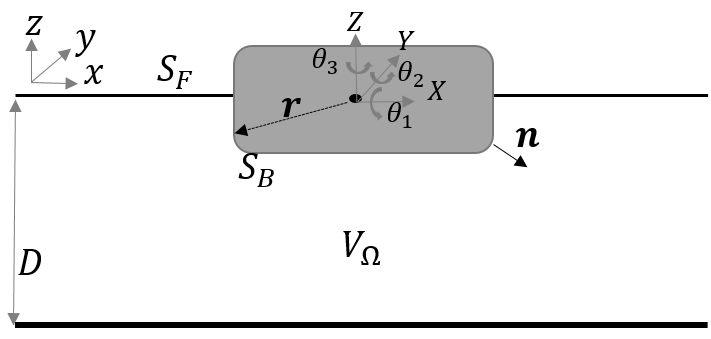
\includegraphics[scale=0.7,trim = 0mm 0mm 0mm 0mm, clip]{figures/Sketch.png}	
\caption{Sketch definition of the system}\label{fig:sketch}
\end{figure}

The floating body has 6 degrees of freedom (DoF), $\bs\xi=(\bs{X},\bs{\theta})$ where the positions, $\bs{X}=(X,Y,Z)$ and the orientations, $\bs{\theta}=(\theta_1,\theta_2,\theta_3)$ are determined at the center of gravity (COG). Displacements of points at the hull are specified by a body of vector $\bs r$ with respect to the COG as $\bs{\mathcal{X}}=\bs{X}+R(\bs{r})$. $R$ is a rotation operator where $R(\bs r)\approx \bs \theta \times \bs r$. The velocity of the points at the hull is expressed as $\dot{\bs{\mathcal{X}}}$.

On the body hull $S_B$, the wetted part is defined as a function $z=\zeta(\vec{x},t)$. The normalized normal vector is defined as directed toward the fluid domain,  $\bs n=-\bs N/|\bs N|$ with $\bs N=\left(-\nabla_2\zeta,1 \right)$ where $\nabla_2$ is the two-dimensional gradient in $\vec{x}$. Then the six-dimensional generalized normal vector is defined as $\bs \nu=(\bs n,\bs r \times \bs n)^T$, with $( )^T$ the matrix transpose operator.

\subsubsection*{Modelling}
NEMOH1, the first-order solver, is based on the following modelling principles:
\begin{itemize}
\item Potential flow theory for an inviscid and incompressible fluid in irrotational motion. The set of equations solved looks for unknowns satisfying free-surface conditions, impermeable bottom condition, diffraction and radiation conditions on the body hull and radiation wave condition in the far field.
\item The harmonic fluid potential is defined as
\begin{align}\label{Eq:PhiHarm}
\Phi(\bs x,t)=Re\left\lbrace\Phi^{(1)}(\bs x)e^{-i\omega t}\right\rbrace.
\end{align}
The total potential, $\Phi$, is the sum of the incident potential, the diffraction potential and the radiation potential. 
The incident potential is defined as, with $k$ and $\omega$ related with the dispersion relation, $\vec{k}=k(\cos \beta,\sin \beta)$, $\beta$ is wave direction and $a$ is a unit wave amplitude, 
\begin{align}\label{Eq:PhiI}
\Phi_{I}^{(1)}(\bs x)=-i\frac{a g}{\omega}\frac{\cosh(k(D+z))}{\cosh(kD)} e^{i\vec{k}\cdot \vec{x}}.
\end{align}
The radiation potential is defined as $\Phi_R(\bs x,t)=Re\left\lbrace \dot{\bs \xi}^{(1)}(t) \cdot \bs \psi(x)\right\rbrace$ where $\bs \psi(\bs x)$ is the normalized vector radiation potential.

\item The three-dimensional linear potential flow problem around arbitrary body condition is reformulated in the Boundary Integral Equation (BIE) and transformed into the two-dimensional problem of the source distribution, $\sigma$, on the body surface, $S_B$, using Green's second identity and the appropriate Green function, $G(\bs x,\bs x')$. 
\item The Green function is based on Delhommeau's formulation and is available for finite and infinite water-depth, see \cite{Delhommeau}.
\item The source distribution depends on the considered boundary condition problem. For each frequency and wave direction, the diffraction source distribution, $\sigma_D(\bs x)$, depends on the position of the panels while the radiation source distribution, $\sigma_{R_j}(\bs x)$,  depends on the position of the panels and the considered degree of freedom $j$.

\item Then, the BIE for $\bs x \in S_B$, is expressed as, with flow points $\bs x$ and source points $\bs x'$,
\begin{align}
\frac{1}{2}\sigma_{D,R_j}(\bs x)-\frac{1}{4\pi}\int_{S_B} \partial_n G(\bs x, \bs x') \sigma_{D,R_j}(\bs x') dS'=\mathcal{N}_{D,R_j}(\bs x). \label{Eq:BIE_source_distribution}
\end{align}
where $\mathcal{N}(\bs x)$ is the body normal condition. The diffraction normal condition is defined as $\mathcal{N}_D (\bs x)=-\partial_{n} \Phi_I^{(1)}(\bs x)$, the normalized radiation condition, $\mathcal{N}_R (\bs x)=\partial_{n} \Phi_{R_j}(\bs x)$, with $\Phi_{R_j}(\bs x)$ is the vector component-$j$ of the normalized radiation potential $\bs \psi(\bs x)$, explicitly $\bs \psi=(\Phi_{R_1},\Phi_{R_2},\cdots,\Phi_{R_{Ndof}})$. 

\item The diffraction potential, $\Phi^{(1)}_{D}$, the normalized radiation  potential vector component-$j$, $\Phi_{R_j}$ and the corresponding velocities are then computed as follows, for the flow points in the fluid domain $\bs x \in S_B \cup V_{\Omega_F}$,
\begin{align} \label{Eq:BIE_Sol_Pot_Sb}
\Phi^{(1)}_{D,R_j}(\bs x)=&-\frac{1}{4\pi}\int_{S_B} G(\bs x, \bs x') \sigma_{D,R_j}(\bs x') dS'\\
\partial_{\bs x} \Phi^{(1)}_{D,R_j}(\bs x)=&\frac{1}{2}\sigma_{D,R_j}(\bs x)\bs{n}\delta_{\bs x \bs x'}-\frac{1}{4\pi}\int_{S_B} \partial_{\bs{x}} G(\bs x, \bs x') \sigma_{D,R_j}(\bs x') dS'
\end{align}  
where the Kronecker delta $\delta_{\bs x \bs x'}=1 $ for $\bs x = \bs x'$, and $\delta_{\bs x \bs x'}=0$ otherwise.
\item The hydrodynamic coefficients are then computed as follows, the excitation force is defined as
\begin{align}
\bs F_{exc}^{(1)}&=\rho \iint_{S_{B}} -i\omega\left[  \Phi_I^{(1)}+ \Phi_D^{(1)}\right]\bs \nu dS.
\end{align}
The added mass matrix and damping coefficient matrix components are computed as
\begin{align}
M^a_{ij}= -\rho \iint_{S_{B}}  \nu_{i} Re \left\lbrace\psi_{R_j} \right\rbrace dS\\
B_{ij}= -\rho \omega \iint_{S_{B}} \nu_{i} Im \left\lbrace\psi_{R_j} \right\rbrace  dS.
\end{align}
\item  In post-processing, the radiation damping impulse response matrix function ($\bs{IRF}(t)$), the infinite frequency added mass matrix ($[\bs M^a](\infty)$), and the excitation force impulse response vector function ($\bs{IRF}_{ex}(t)$) are provided. They are computed as, 
\begin{align*}
\bs{IRF}(t)&\approx\frac{2}{\pi}\int_0^{\omega_{max}}[\bs B](\omega)\cos(\omega t)d\omega, \\
[\bs M^a](\infty)&\approx  \frac{1}{N_{\omega}}\sum_{i=1}^{N_{\omega}}[\bs M^a](\omega_i)+\int_0^{t_{max}}\bs{IRF}(t)\sin(\omega_i t)dt\\
\bs{IRF}_{exc}(t)&\approx\frac{1}{2\pi}\int_{-\omega_{max}}^{\omega_{max}}\bs F_{exc}(\omega)e^{-i\omega t}d\omega.
\end{align*}
where $\bs F_{exc}(-\omega)=\bs F^*_{exc}(\omega)$. Note that $\omega_{max}$ is a user-specified input, for better accuracy of $\bs{IRF}(t)$ make sure that $[\bs B ](\omega_{max})$ has reached an asymptotic value.
\item Response Amplitude Operators (RAO) are obtained by solving the following equation of motion
\begin{align}\label{Eq:RAO}
\left[-[\bs M+\bs M^a(\omega)]\omega^2-i\omega[\bs B(\omega)+\bs B_{add}]+[\bs K_h+\bs K_M]\right]\mathcal{\bs \xi}(\omega)=\bs F_{exc}(\omega)
\end{align}
where $[\bs B_{add}]$ and $[\bs K_M]$ are user-specified additional damping and stiffness matrices.
\end{itemize}
\ \\
NEMOH2, the second-order QTF module, is based on the following principles
\begin{itemize}
\item The second-order loads are composed of the quadratic part and the potential part, the detailed formulation is given in \cite{Kurnia22_JH,Kurnia22}.
\item The quadratic part is based on the near-field method \cite{CHEN88}. 
\item The potential part is based on the 
indirect method \cite{CHEN88,MOLIN79}.
\end{itemize}

\subsubsection*{Numerical Methods}

NEMOH1 uses the following numerical approach:
\begin{itemize}
\item The BIE, Eq. \eqref{Eq:BIE_source_distribution}, is discretised using the constant panel method with quadrilateral mesh. This leads to a linear system with the influence coefficients matrix. The mesh is user-specified with the normal direction towards fluid.
\item Numerical implementation of the Green function is described in \cite{Babarit15}.
\item Free-surface Green function integrands are pre-calculated with the discretized $\omega^2r/g\in [0,100]$ with 676 points in a constant scale and $\omega^2(z+z')/g \in [-251,-1.6\, 10^{-6}]$ with 130 points in logarithmic scale. A polynomial surface interpolation with the $5^{th}$ order Lagrange formula is used for interpolating any values in the specified interval.

\item The specified points for the interpolation of the Green function are finer than in the previous release. However, an option to switch the two different tabulated Green function data is available in the source file \texttt{\textbackslash Solver\textbackslash Core\textbackslash INITIALIZE\_GREEN.f90} with the parameter FLAG\_IGREEN=1 or 2, 2 being the default. 

\item Influence coefficients, the integration of $\partial_n G(\bs x, \bs x')$ over a body panel, is computed using  Gauss-quadrature integration with a user-input number of Gauss-quadrature points.

\item The source distributions on body panels are then obtained after solving the corresponding linear system. 

\item The linear system is solved using a user-choice solver among the available ones, which are Gauss elimination, LU-decomposition (default) and GMRES-iterative solvers.

\item The GMRES solver code \cite{GMRES} from \href{https://www.cerfacs.fr/algor/Softs/GMRES/index.html}{\underline{CERFACS}} is embedded in NEMOH solver module. For using the GMRES solver, the user has to obtain a license in \url{https://www.cerfacs.fr/algor/Softs/GMRES/license.html}.

\item For free-surface piercing bodies problem, the irregular frequencies removal (IRR) method is applied by the user providing lid panels at $z=0$. Then, the extended boundary integral equation will be solved \cite{Babarit15,Malenica98}. As in \cite{Malenica98}, the IRR may be influenced by the input parameter $\epsilon$ in \texttt{input\_solver.txt} that shifts the lid panels from $z=0$ to $z=-\epsilon d_B$ where $d_B$ is a maximum horizontal distance of points on the body. $d_B$ is computed by the software.

\item RAO in Eq. \ref{Eq:RAO} is obtained by applying the inverse matrix using LU-decomposition.

\item The software can solve multi-bodies problems, as well as multi-directional waves.
\end{itemize}
\ \\ %newline after itemize
NEMOH2 uses the following numerical approach
\begin{itemize}
\item The QTF module can be run only after the first order-hydrodynamic coefficients are computed in NEMOH1.
\item In the potential part, the computation of the free-surface integral is an option: 
\begin{itemize}
    \item For the difference-frequency QTFs, it is in general acceptable not to compute the free-surface integral terms.
    \item For the sum-frequency QTFs, it is necessary to compute the free-surface integrals.
\end{itemize}
\item Important notice: the computation with the free-surface integral still has an issue if the lid body panels exist (cf. IRR method). For now, the user is suggested not to specify the lid body panels in the mesh file input for NEMOH1 computation if he wants to compute the full QTFs with the free surface integral.
\item For the free-surface integral, a quadrilateral free-surface mesh has to be specified.
\item The computation can be done for bi-directional or uni-directional wave for the specified multiple wave direction.
\item QTF computations have not been tested yet for the multi-bodies problem.
\end{itemize}
\ \\
NEMOH related publications to be referred are  \cite{Babarit15} for the first order NEMOH and \cite{Philippe15,Kurnia22_JH,Kurnia22} for the QTF module. A publication related with this release is in preparation as in \cite{Kurnia23}.
\subsection{Units}
NEMOH expects all quantities to be expressed in S.I. units: $m, kg, s, rad$ (meter, kilogram, seconds, radian, respectively). But some of the phase outputs may be expressed in $deg$ or $^{\circ}$, in this case it will be indicated in the file header.

The force unit is [$N$], the moment unit is [$Nm$], added Mass [$kg$], damping coefficient [$kg/s$]. As the force output is normalized with the unit wave amplitude $a$ $[m]$, then the normalized force unit is [$N/m$] and the normalized moment is [$N$]. 

Response amplitude operator for translation motion has unit [$m/m$] and for rotation it is [$deg/m$]. 

The force quadratic transfer function (QTF) has unit [$N/m^2$] and for the moment QTF it is [$N/m$]. The QTF output is normalized by $\rho g$ where the fluid density $\rho,\ [kg/m^3],$ and the gravitation constant $g,\ [m/s^2]$.

\subsection{Software    features and capabilities}
\begin{figure}[ht]
\centering
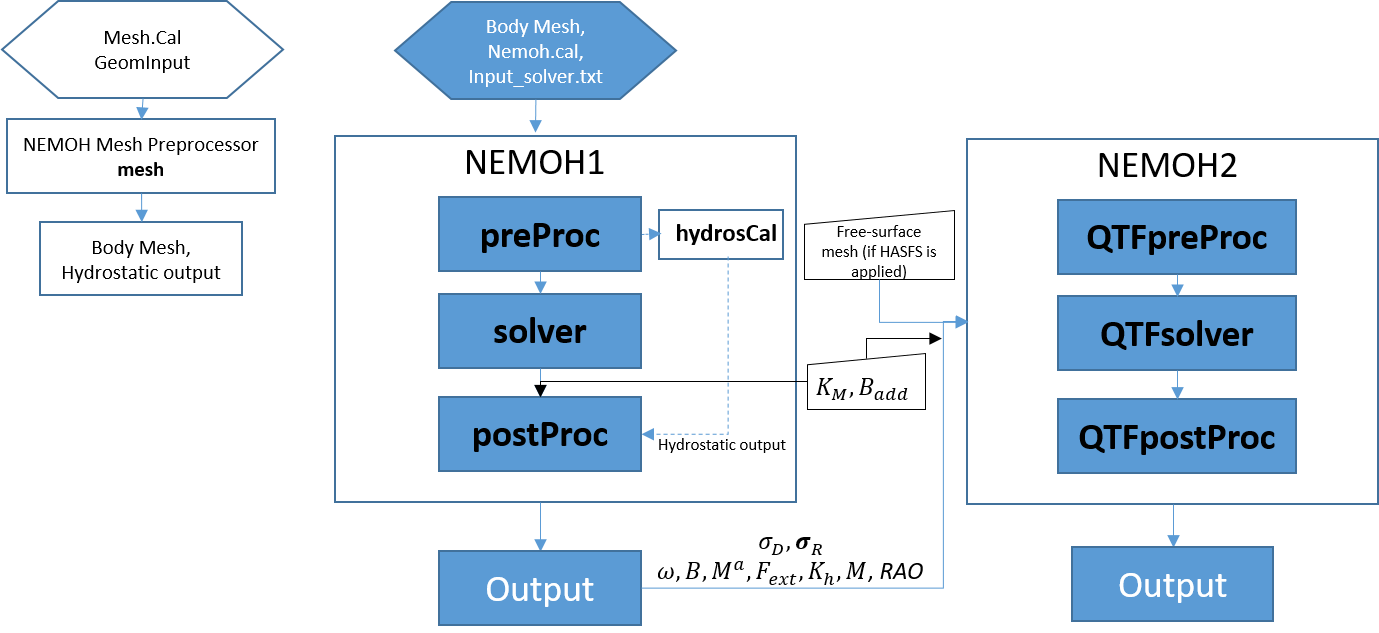
\includegraphics[scale=0.6,trim = 0mm 0mm 0mm 0mm, clip]{figures/FlowChart.png}	
\caption{Global flowchart of NEMOH software}\label{fig:flowchart}
\end{figure}

Fig. \ref{fig:flowchart} shows a global overview of the software. There are three main programs: a mesh preprocessor, NEMOH1 and NEMOH2. The program features and capabilities are described as follows.

\subsubsection{Mesh Preprocessor}
NEMOH mesh preprocessor, the executable file \texttt{\textbf{mesh}}, is for generating the NEMOH mesh file with a given geometry input file and an input \texttt{Mesh.cal} file. This \texttt{\textbf{mesh}} is not a meshing code but allows the user to refine an existing mesh and to calculate properties such as displacement, buoyancy center, and hydrostatic stiffness. It also makes estimates of masses and inertia matrix. The concept with this program is to write by hand a coarse description of the body under consideration in a \texttt{GeomInput} file and to have \texttt{\textbf{mesh}} make the refined mesh for NEMOH calculations.

\subsubsection{NEMOH1: 1st-order solver}
NEMOH1 solves the first-order potential flow problem. There are four modules: \texttt{\textbf{preProc}}, \texttt{\textbf{hydrosCal}}, \texttt{\textbf{solver}} and \texttt{\textbf{postProc}}, described as follows.
\begin{itemize}
\item \texttt{\textbf{preProc}}: processes the input mesh file and generates the body condition for each calculation case (diffraction and radiation). The outputs are used as input for \texttt{\textbf{solver}}.
\item \texttt{\textbf{hydrosCal}}: computes hydrostatic parameters, i.e. stiffness matrix and inertia matrix. The output file will be used in the \texttt{\textbf{postProc}} for computing the RAOs. If the input mesh is generated by the NEMOH mesh preprocessor, \texttt{\textbf{mesh}}, the hydrostatic parameters are already computed and then it is not necessary to execute this program. 
\item \texttt{\textbf{solver}}: solves the boundary value problems for each problem, diffraction and radiation, defined in the file \texttt{Normalvelocities.dat}, provided by the \texttt{\textbf{preProc}}. 
\begin{itemize}
\item  The influence coefficients matrix is constructed with the infinite/finite depth Green function.
\item If a finite depth is specified, then the finite depth green function is applied only for $\frac{\omega^2}{g}D<20$, otherwise infinite depth case is applied.
\item The integration of the Green function on a panel for the influence coefficients is obtained by the Gauss-quadrature integration. The number of Gauss quadrature points is a user input. 
\item The minimum distance, $\epsilon$, between the flow and source points for the influence coefficient computation is user-specified.
\item The source distributions are then obtained by solving the linear system. There are three options for the solver: Gauss elimination, LU-decomposition and GMRES.  If the GMRES solver \cite{GMRES} is used and the target tolerance is not achieved after the maximum number of iterations, the problem is automatically solved by LU-decomposition. License for using GMRES has to be obtained in \url{https://www.cerfacs.fr/algor/Softs/GMRES/license.html}.
\end{itemize}

\item \texttt{\textbf{postProc}}: post-processes the \texttt{\textbf{solver}}'s output files. The results are the excitation forces, added mass and damping coefficients. Optionally, the program computes 
\begin{itemize}
\item the radiation damping impulse response function, the infinite frequency added mass and the excitation force impulse response function,
\item the Kochin coefficient,
\item the free-surface elevation,
\item the motion response amplitude operator (RAO). For the RAO computation, additional stiffness matrix $[\bs K_m]$ and additional damping $[\bs B_{add}]$ can be user-specified in the \texttt{Mechanics/} folder.
\end{itemize}
\end{itemize}
\subsubsection{NEMOH2: 2nd-order QTF module}
NEMOH2 computes the second-order wave loads that are expressed as Quadratic Transfer Function (QTF). It is suggested to verify the first-order results before running the QTF module. There are three modules in this program: \texttt{\textbf{QTFpreProc}}, \texttt{\textbf{QTFsolver}} and \texttt{\textbf{QTFpostProc}}, described as follows
\begin{itemize}
\item \texttt{\textbf{QTFpreProc}}: computes the perturbed potential, the total potential, the normalized radiation potential and the corresponding velocities on the body panels, the water-line and the free-surface panels. 
\begin{itemize}
\item The computation on free-surface panels requires possibly long computational time. Then, it is suggested not to compute the free-surface integral for the first execution of NEMOH2. This is controlled by the flag HASFS, which is available in the input file \texttt{Nemoh.cal}.
\item In general, the free-surface integral may be negligible for the difference-frequency QTFs computation.
\item The potential on the waterline is rather sensitive with the $\epsilon$ value. For default, $\epsilon=0.001$, it can be adjusted in \texttt{input\_solver.txt}. The $\epsilon$ can be set differently for NEMOH1 and NEMOH2. Further investigation into this is needed.
\item In case the body lid panels exist, the influence coefficients are affected and give a somewhat larger error for higher frequencies on the free-surface potentials and velocities. This also needs to be investigated.
\item For now, in the case of full-QTFs computation, the user is suggested not to specify the lid body panels in a mesh file input for NEMOH1 computation.
\end{itemize}
\item \texttt{\textbf{QTFsolver}}: computes the quadratic part and the potential part of the second order loads. The free-surface integrals in the potential part QTF are optionnally computed (flag HASFS in \texttt{Nemoh.cal}).
\item \texttt{\textbf{QTFpostProc}}: adds all the computed QTF parts and produces the total QTF. The option to sum only some parts of the QTF is available in \texttt{Nemoh.cal}.
\end{itemize}

\section{Getting-started} \label{Sec:Getstarted}
This section describes the installation procedure and how to run the codes. It also includes a description of input-output files.

%The installation and running procedures in this section are intended for Linux platforms. An updated manual will provide similar information for Windows platforms. But in this Release, the executable files are provided both for Linux and Windows platforms.

\subsection{Executable files}\label{Sec:Execute}
Executable/binary files are provided in the \texttt{Release} section of the \href{https://gitlab.com/lheea/Nemoh}{GitLab project}. They can be used directly without the need to do the compilation procedure described in the next subsection. Windows and Linux executable files are provided. In the case of a compilation on your computer, executable files will be located in the \texttt{bin/} folder. \\

\noindent
The following executable files are available:
\begin{itemize}
\item NEMOH1: \texttt{\textbf{mesh}}, \texttt{\textbf{preProc}}, \texttt{\textbf{hydrosCal}}, \texttt{\textbf{solver}}, \texttt{\textbf{postProc}},
\item NEMOH2: \texttt{\textbf{QTFpreProc}}, \texttt{\textbf{QTFsolver}}, \texttt{\textbf{QTFpostProc}}.
\end{itemize}

Note that a Matlab wrapper is provided to use those executable files in a Matlab environment. More details are provided in Sec. \ref{Sec:MatlabFiles}.

\subsection{Installation}
This procedure is intended for a developer to perform the compilation after changing the source code. Users may skip this step.

As a first preliminary step, it is necessary to install the following external libraries that are used by NEMOH:
\begin{itemize}
    \item BLAS, \url{https://netlib.org/blas/}
    \item LAPACK, \url{https://netlib.org/lapack/}
\end{itemize}

\subsubsection{Windows platform}
An updated manual will provide the details of the compilation on a Windows platform.

\subsubsection{Linux platform}
Before compiling, the following tools need to be available:
\begin{itemize}
    \item A Fortran compiler. The code has been tested using:
    \begin{itemize}
        \item gfortran, \url{https://gcc.gnu.org/wiki/GFortran}, 
        \item intel fortran compiler, \href{https://www.intel.com/content/www/us/en/developer/tools/oneapi/fortran-compiler.html#gs.jik1s6}{ifort}.
    \end{itemize}
    \item CMake, \url{https://cmake.org/}, a cross-platform tool for building and testing the software package.
\end{itemize}

\noindent
Compile all Nemoh executables using CMake (from the root of the repository):
\begin{lstlisting}[language=bash,keywordstyle=\color{blue},basicstyle=\ttfamily\footnotesize,backgroundcolor=\color{lightgray}]
    cmake -S. -Bbuild
    cmake --build build
\end{lstlisting}
The resulting executables are in the \texttt{bin/} directory. To compile only one of the executables, use the \texttt{--target} option of CMake. The available targets are:
\begin{itemize}
    \item for NEMOH: \texttt{{mesh}}, \texttt{{preProc}}, \texttt{{hydrosCal}}, \texttt{{solver}}, \texttt{{postProc}}
    \item for NEMOH QTF:\texttt{{QTFpreProc}}, \texttt{{QTFsolver}}, \texttt{{QTFpostProc}}
\end{itemize}

The choice of the compiler is left to CMake, but can be overridden by setting the \texttt{CMAKE\_Fortran\_COMPILER} at the configuration step, e.g.:
\begin{lstlisting}[language=bash,keywordstyle=\color{blue},basicstyle=\ttfamily\footnotesize,backgroundcolor=\color{lightgray}]
    cmake -S. -Bbuild -DCMAKE_Fortran_COMPILER=gfortran
\end{lstlisting}
\vspace*{5mm}

\noindent
After building, the tests can be run from the \texttt{build/} directory:
\begin{lstlisting}[language=bash,keywordstyle=\color{blue},basicstyle=\ttfamily\footnotesize,backgroundcolor=\color{lightgray}]
    ctest -V -j <N_concurrent>
\end{lstlisting}

Where \texttt{<N\_ concurrent>} is the number of simultaneous workers (processes). The tests can be restricted using their labels and the \texttt{-L} option of ctest:
\begin{lstlisting}[language=bash,keywordstyle=\color{blue},basicstyle=\ttfamily\footnotesize,backgroundcolor=\color{lightgray}]
    ctest -V -j <N_concurrent> -L <label>
\end{lstlisting}

Where label is one of the following:
\begin{itemize}
    \item \texttt{NEMOH1}: only the non-QTF test cases
    \item \texttt{PREPROC}: only the pre-processing operations
    \item \texttt{SOLVER}: only the solving operations (depend on the pre-processing tests)
    \item \texttt{POSTPROC}: only the post-processing operations (depend on the pre-processing and solving tests)
    \item \texttt{NEMOH2}: only the QTF test cases
    \item \texttt{QTF}: only the computation of the QTF (depend on the prior non-QTF Nemoh computation)
\end{itemize}
Tests with unsatisfied requirements will fail.

\subsection{Running}
The binary files of NEMOH1 and NEMOH2 have to be executed following the order provided in Sec. \ref{Sec:Execute}. %If the binary file exists but there is no access to be executed, in the command window type chmod +x 'binfile' that will add the executable access to the 'binfile'.  

The following steps are for executing the binary files in the command window.
\begin{itemize}
\item Suppose a project directory, \emph{e.g.} \texttt{/NEMOH/projdir/}, that contains all the input files and that is in the same location as the binary directory, i.e \texttt{NEMOH/bin/}. 
\item The program can be run depending on your current working directory in the command line. For example, the following commands are possible, with \texttt{\textbf{binfile}} being an executable file i.e. \texttt{\textbf{preProc}}, etc., as
\begin{itemize}
\item if you are in the \texttt{projdir}:
\begin{lstlisting}[language=bash,keywordstyle=\color{blue},basicstyle=\ttfamily\footnotesize,backgroundcolor=\color{lightgray}]
    ./../bin/binfile
\end{lstlisting}
\item if you are in the {bin}:
\begin{lstlisting}[language=bash,keywordstyle=\color{blue},basicstyle=\ttfamily\footnotesize,backgroundcolor=\color{lightgray}]
    ./binfile ./../projdir
\end{lstlisting}
\end{itemize}
\end{itemize}

Before executing the binary files, the input files are needed. These are described in the next subsection.\\

Finally, a set of test cases are provided. The results are presented in Sec. \ref{Sec:Testcase} and we provide here the methodology to run those tests. The first possibility is to run each of the cases in the command line, following the above instructions. This applies to both Windows and Linux environments.

To simplify the procedure for Linux platforms, \texttt{Makefile} is provided in the \texttt{TestCases/} directory. It is then possible to run the NEMOH1 test cases by executing the following commands in a Terminal (each line being a test case):
\begin{lstlisting}[language=bash,keywordstyle=\color{blue},basicstyle=\ttfamily\footnotesize,backgroundcolor=\color{lightgray}]
make run_1_cylinder
make run_2_2Bodies
make run_3_nonsymmetrical
make run_4_postprocessing
make run_5_quicktest
make run_6_box_coarsemesh
make run_7_Solvers_Check_OC3
make run_8a_Cylinder_irregfreq
\end{lstlisting}

For the QTF test cases, the following commands can be used:
\begin{lstlisting}[language=bash,keywordstyle=\color{blue},basicstyle=\ttfamily\footnotesize,backgroundcolor=\color{lightgray}]
make run_8b_QTF_Cylinder
make run_9_oc4_semisub
make run_10a_softwind
make run_10b_softwind_FS
make run_11_QTF_OC3_Hywind.
\end{lstlisting}

Commands to clean the test cases are also available to clean all the output files. They can apply either to a specific tests case, \emph{e.g.} 
\begin{lstlisting}[language=bash,keywordstyle=\color{blue},basicstyle=\ttfamily\footnotesize,backgroundcolor=\color{lightgray}]
make clean_1_cylinder
\end{lstlisting}

Or to remove a range of test cases
\begin{lstlisting}[language=bash,keywordstyle=\color{blue},basicstyle=\ttfamily\footnotesize,backgroundcolor=\color{lightgray}]
make clean_all_testsNEMOH1
make clean_all_testsNEMOH2
make clean_all_tests
\end{lstlisting}

The description and the benchmark results of those test cases are described in Sec. \ref{Sec:Testcase}.

\subsection{Input/Output}

Following is the list of the user's input files and the output files for each executable file:
\begin{itemize}
\item \texttt{\textbf{mesh}}
\begin{itemize}
\item User's input files: \texttt{projdir/Mesh.cal}, \texttt{projdir/geomInput}, 
\item Output files: \texttt{projdir/meshfile}, \texttt{projdir/mesh/[*.dat, *.tec]},
\end{itemize}
\item \texttt{\textbf{preProc}}
\begin{itemize}
\item User's input files: \texttt{projdir/Nemoh.cal}, \texttt{projdir/meshfile}, 
\item Output files: \texttt{projdir/Normalvelocities.dat}, \\
  \hspace{2cm} \texttt{projdir/results/[FKForce.dat, FKForce.tec, index.dat]}, \\
  \hspace{2cm} \texttt{projdir/mesh/[L10.dat, L12.dat]},
\end{itemize}
\item \texttt{\textbf{hydrosCal}}
\begin{itemize}
\item User's input files: \texttt{projdir/Nemoh.cal}, \texttt{projdir/mesh.cal},
\item Output files: \texttt{projdir/mesh/[*.dat, *.tec]}, \texttt{projdir/Mechanics/},
\end{itemize}
\item \texttt{\textbf{solver}}
\begin{itemize}
\item User's input files: \texttt{projdir/Nemoh.cal}, \texttt{projdir/input\_solver.txt}  
\item Output files: \texttt{projdir/results/Forces.dat},\\
\texttt{projdir/results/sources} (if QTF will be computed, indicated in \texttt{Nemoh.cal})
\end{itemize}
\item \texttt{\textbf{postProc}}
\begin{itemize}
\item User's input files: \texttt{projdir/Nemoh.cal}, \\ \texttt{projdir/Mechanics/[Km.dat,Badd.dat]}  
\item Output files: \texttt{projdir/results/[ExcitationForce.tec,}\\
\texttt{DiffractionForce.tec,RadiationCoefficients.tec,$\cdots$]},\\ \texttt{projdir/Motion/RAO.dat},
\end{itemize}
\item \texttt{\textbf{QTFpreProc}}
\begin{itemize}
\item User's input files: \texttt{projdir/Nemoh.cal}, \texttt{projdir/FSmeshfile} (If the free-surface integral, HASFS flag, is computed), \\ \texttt{projdir/Mechanics/[Km.dat,Badd.dat]}
\item Output files: \texttt{projdir/QTFPreprocOut/*.bin},
\end{itemize}
\item \textbf{QTFsolver}
\begin{itemize}
\item User's input files: \texttt{projdir/Nemoh.cal}
\item Output files: \texttt{projdir/results/QTF/*.dat},
\end{itemize}
\item \textbf{QTFpostproc}
\begin{itemize}
\item User's input files: \texttt{projdir/Nemoh.cal}
\item Output files: \texttt{projdir/results/QTF/[OUT\_QTFM\_N.dat,OUT\_QTFP\_N.dat]}
\end{itemize}
\end{itemize}
\ \\
As summary, following files are needed for the input, some depends on user-specified choice in \texttt{Nemoh.cal}:
\begin{itemize}
\item \texttt{Nemoh.cal} contains all NEMOH computation parameters
\item \texttt{Mesh.cal} contains information of \texttt{geomInput} file. It is an input for \texttt{\textbf{mesh}} and \texttt{\textbf{hydrosCal}}.
\item a \texttt{meshfile}, input for \texttt{\textbf{preProc}}, or \texttt{geomInput} file, input for \texttt{\textbf{mesh}}
\item  \texttt{input\_solver.txt} contains \texttt{\textbf{solver}} parameters
\item \texttt{Km.dat} and \texttt{Badd.dat}, are the additional stiffness and damping matrices. These optional input are for \texttt{\textbf{postProc}}/\texttt{\textbf{QTFpreProc}}
\item \texttt{{FSmeshfile}} contains the free-surface mesh if contrib=3 in \texttt{Nemoh.cal}.
\end{itemize}
\ \\
NEMOH produces the following main output files, some depending on user-specified choice in \texttt{Nemoh.cal}, 
\begin{itemize}
\item hydrostatic files: inertia and stiffness matrices, 
\item hydrodynamics coefficients: Froude-Krylov force, excitation force, added-mass, damping coefficient,
\item Kochin function, free-surface elevation,
\item Response Amplitude Operator (RAO),
\item Total difference- and sum-frequencies QTFs.
\end{itemize}
\ \\
Detail descriptions of the input/output files are discussed in the next subsections.

\subsubsection{User's input files}

\begin{figure}[ht]
\centering
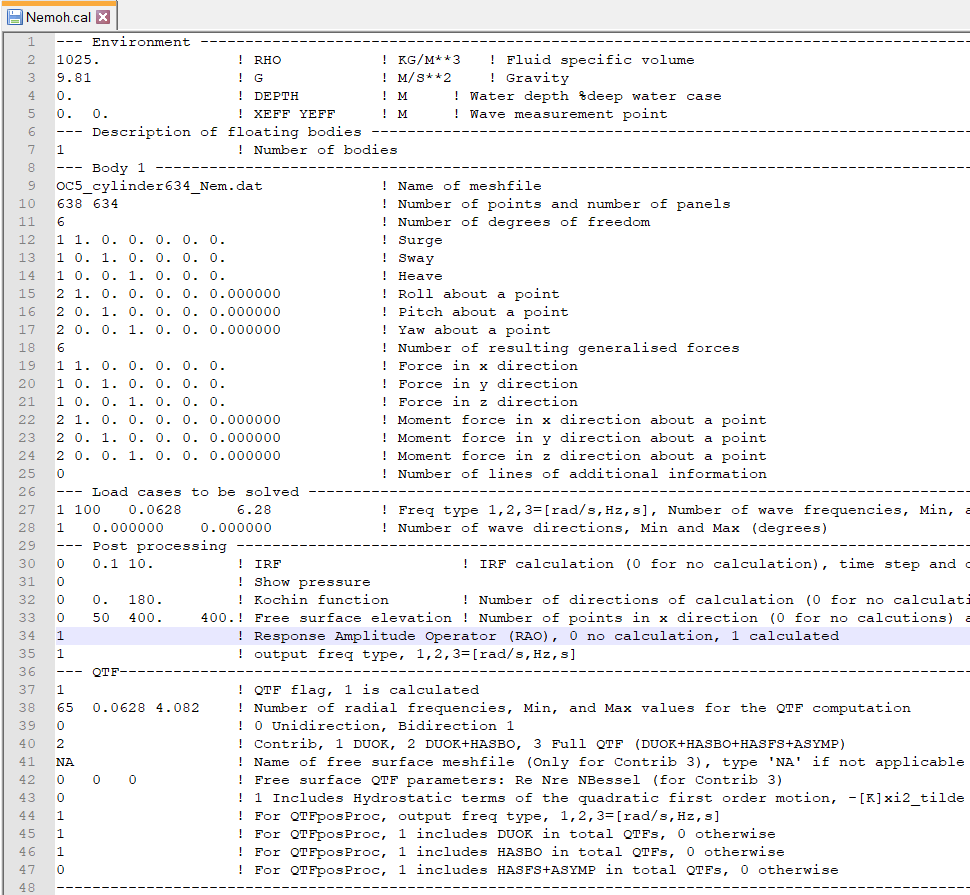
\includegraphics[scale=0.8,trim = 0mm 0mm 12mm 0mm, clip]{figures/NemohCal.png}	
\caption{\texttt{Nemoh.cal} input file}\label{fig:NemohCal}
\end{figure}

\texttt{Nemoh.cal}: contains all computation parameters with the format as in Fig. \ref{fig:NemohCal}. The following parameters have to be specified:
\begin{itemize}
\item \emph{Environment}: fluid density, gravity constant, water-depth and wave reference point.  Specify $0.$ for infinite water depth case.
\item \emph{Description of floating bodies}: number of bodies, name of the \texttt{meshfile}, number of points and number of panels, number of degrees of freedom, motion description, number of resulting generalized forces and its description.
\begin{itemize}
\item \texttt{meshfile} has to be provided in the folder \texttt{projdir/}
\item Number of points and panels correspond with the data in the \texttt{meshfile}
\item For each motion and resulting generalized force, 7 parameters have to be specified in a row. The first parameter, 1 for translation motion/force, 2 for rotation motion/force. The second to fourth parameters is a unit vector of motion/force, 1 0 0 for surge/roll, 0 1 0 for sway/roll, 0 0 1 for heave/yaw. The fifth to seventh parameters are the reference point coordinate $(x,y,z)$.
\item In the multibody cases, all the parameters have to be specified in rows for each body.
\end{itemize}
\item \emph{Load case to be solved}: contains wave frequency and wave direction parameter.
\begin{itemize}
\item Four wave frequency parameters have to be specified in a row. First, the frequency type, 1 for radial-frequency [rad/s], 2 for frequency [Hz] and 3 for period [s]. The second to fourth parameters are the number of frequencies/periods, and their minimum and maximum values.
\item In the case of QTF computation, it is suggested that the computed first-order hydrodynamic coefficients in NEMOH1 cover all difference-frequencies and sum-frequencies intervals for the QTF computation. The suggested radial frequency interval is $\omega \in [\Delta \omega, \omega_{max}]$ with a step $\Delta \omega$,  $\omega_{max}=N_{\omega}\Delta \omega$ and $N_{\omega}$ is the total number of radial frequencies. The $\omega_{max}$ should be chosen as the maximum computed sum-frequencies, $\omega_1+\omega_2$.
\item The wave direction parameters are the number of directions, and the minimum and maximum angle directions [deg].
\end{itemize}
\item \emph{Post processing} contains parameters for Impulse Response Functions, pressure, Kochin, free surface elevation, RAO and frequency type output.
\begin{itemize}
\item The IRFs computation requires 3 parameters; a switch [0 is not calculated, 1 calculated], a time-step and a maximum time.
\item A switch pressure parameter [0 is not calculated, 1 calculated].
\item The Kochin parameters are a number of directions (specify 0 if it is not calculated), minimum and maximum values of angle directions [deg].
\item The free surface parameters are the number of points in $x$-direction (specify 0 if it is not calculated) and $y$-direction, the dimension of the domain in $x$ and $y$ directions [m].
\item A switch for RAO computation [0 is not calculated and 1 is calculated]. If QTF will be computed, the RAO has to be computed and then the switch has to be set to 1.
\item Frequency output option: 1 for the radial frequency [rad/s], 2 for the frequency [Hz] and 3 for the period [s]. 
\end{itemize}
\item \emph{Quadratic Transfer Function (QTF)} contains following parameters
\begin{itemize}
\item A flag to decide if QTFs are computed (1) or not (0). If flag=1, then the NEMOH1 module produces the source-distribution file for each problem, which is saved in \texttt{/projdir/results/source}.
\item The frequency parameters are provided only in radial frequency [rad/s] under the form of: the number of frequencies, and minimum and maximum values. The values are not necessarily the same as the input in NEMOH 1 but should be within the range of NEMOH1 input, then an interpolation may be applied.
\item A flag to choose between uni-directional (0) and bi-directional (1) computations of QTFs. If multi-directions are computed in NEMOH1, all the direction interactions will be computed for the bi-directional case. In the uni-directional case, only the same-direction interaction, $\beta_1=\beta_2$, will be computed.
\item Contribution parameter: 1 computes only the quadratic terms of QTFs (referenced as DUOK), 2 computes the quadratic and the body force contribution in the potential QTFs referenced as DUOK+HASBO), 3 includes the computation of the free-surface integrals in the finite domain and semi-infinite domain (this is referenced as DUOK+HASBO+HASFS+ASYMP).
\item If Contrib=3, a free-surface mesh file name has to be specified and the file is placed in \texttt{/projdir/mesh}. Type NA if it is not applicable, Contrib$<3$.
\item If Contrib=3, specify the free-surface parameters: an external radius, $R_e$ is the maximum radius as in the free-surface mesh, a number of discretized radius points in between the waterline $R_b$ and the external radius,  $[R_b,R_e]$, and the number of Bessel functions. The number of Bessel functions is used during the computation in the semi-infinite integral, specify 30 as a default value.
\item Switch 1 for adding to the quadratic QTF (DUOK) the Hydrostatic terms of the quadratic first-order motion, $-[\bs K] \tilde{\bs \xi}^{(2)}$, where, with $z_G$ is the vertical component of CoG,
\begin{align*}
\tilde{\bs\xi}^{(2)}=[0,0,z_G(\theta_1^{(1)2}+\theta_2^{(1)2})/2,\theta_2^{(1)}\theta_3^{(1)}/2,-\theta_3^{(1)}\theta_1^{(1)}/2,0]^T.
\end{align*}  
Note that this term is optional and needed only in QTFsolver. In other software this term is not always included, \emph{e.g.} HYDROSTAR \cite{HYDROSTAR} does not included it.
\item Frequency output option: 1 for the radial frequency [rad/s], 2 for the frequency [Hz] and 3 for the period [s].
\item In \texttt{\textbf{QTFpostproc}}, QTFs total is calculated with summation of all the terms. Option to exclude/include the terms are available with the corresponding switch for DUOK, HASBO and HASFS+ASYMP terms. Switch 1 to include, 0 to exclude. If Contrib=2, then HASFS+ASYMP switch has to be 0.
\end{itemize}
\end{itemize}
\

\noindent
\texttt{meshfile}: contains all the mesh information with a format as shown in Table \ref{tab:meshfile}. Lid panels ($z=0$) of the structure may be included in this file to activate the irregular frequencies removal method. This mesh file may be generated by NEMOH \textbf{\texttt{mesh}} preprocessor or by an external mesh generator.
External mesh generators, \emph{e.g.} the open-source software GMSH \cite{gmsh}, may be used to generate mesh files but they must be adapted to the NEMOH format. A Matlab file for converting GMSH mesh file to the NEMOH format is provided in the dedicated repository. The Matlab file will be described in the next section.\\

\begin{table}[ht]
\begin{center}
\caption{\texttt{meshfile} format}\label{tab:meshfile}
\begin{tabular}{ccccl}
\hline
2 & 1&\ &\ & First column must be a 2.\\
\ &\ &\ &\ & Second column is 1 if half symmetric body mesh, about ($xOz$),\\
\ &\ &\ &\ & specified, 0 otherwise.\\
\hline
1 & $x_1$& $y_1$ &$z_1$ & Table of nodes. First column is node ID.\\
\ &\ &\ &\ & Other columns are the node coordinates $(x,y,z)$\\
\hline
: & :&  :& : & All nodes coordinated listed in the rows\\
\hline
0 & 0.&  0.& 0.& Last line of table of nodes\\
\hline
1 & 2& 3 & 4 & Table of connectivities. Number of node IDs\\
\hline
: & :&  :& : & Connectivities in each panel listed in the rows\\
\hline
0 & 0&  0& 0& Last line of table of connectivities\\
\hline
\end{tabular}
\end{center}
\end{table}

\noindent
\texttt{geomInput}: contain coarse description of mesh, that are number of nodes, number of panels, table of nodes and table of connectivities. The input file has to follow the format as shown in Table \ref{tab:geomInput}.\\

\begin{table}[ht]
\begin{center}
\caption{\texttt{geomInput} file format}\label{tab:geomInput}
\begin{tabular}{ccccl}
\hline
100 &\ &\ &\ & Total number of nodes.\\
\hline
25 &\ &\ &\ & Total number of panels.\\
\hline
$x_1$& $y_1$ &$z_1$ &\ &Table of nodes. \\
\    &\      &\     &\ & The node coordinates $(x,y,z)$\\
\hline
 :& :&  :&\ & All nodes coordinated listed in the rows\\
\hline
1 & 2& 3 & 4 & Table of connectivities. Number of node IDs\\
\hline
: & :&  :& : & Connectivities in each panel listed in the rows\\
\hline
\end{tabular}
\end{center}
\end{table}

\noindent
\texttt{Mesh.cal:} contains mesh and environmental parameters with a format as in Table \ref{tab:meshcal}. This file is used as input for \textbf{\texttt{mesh}} and \textbf{\texttt{hydroCal}}. All the parameters are used in \textbf{\texttt{mesh}}. Only center of gravity, water density, and gravity are used in \textbf{\texttt{hydroCal}}.\\

\begin{table}[ht]
\begin{center}
\caption{\texttt{Mesh.cal} file format}\label{tab:meshcal}
\begin{tabular}{ccccl}
\hline
geomInput\_name &\ &\ &\ & Name of the geomInput file.\\
\hline
0 &\ &\ &\ & 1 if a half symmetric body mesh, about ($xOz$), specified.\\
\hline
0. &0. &\ &\ & Possible translation about x axis (first column)\\
\    &\      &\     &\ & and y axis (second column)\\
\hline
0. &0. &-7 &\ & Coordinates of gravity centre \\ 
\hline
500. &\ &\ &\ & Target for the number of panels in refined mesh \\ 
\hline
2. &\ &\ &\ &  \\ 
\hline
0. &\ &\ &\ &  \\ 
\hline
1. &\ &\ &\ &  \\ 
\hline
1025 &\ &\ &\ & water density $(kg/m^3)$\\
\hline
9.81 &\ &\ &\ &gravity $(m/s^2)$\\
\hline
\end{tabular}
\end{center}
\end{table}

\noindent
\texttt{input\_solver.txt} contains solver parameters with format as in Table \ref{tab:input_solver}. The parameters are described as follows.
\begin{itemize}
\item Number of Gauss Quadrature points, $N^2$, is used for the surface integration in the influence coefficients. User specifies an integer value of $N\in [1,4]$, default $N=2$.
\item Minimum z of flow and source points is defined with a factor  $\epsilon_{zmin}$ multiplied by the maximal horizontal distance between two point of the mesh, default $\epsilon_{zmin}=0.001$. 
\item Three linear-system solvers are available; 1 Gauss elimination, 2 LU Decomposition, 3 GMRES iterative solver.
\item If GMRES solver is chosen then the three parameters, the restart parameter, the relative tolerance and the maximum number of iterations, have to be specified. If the tolerance is not achieved after the maximum iteration exceeded then LU decomposition solves the system directly.\\
\end{itemize}

\begin{table}[ht]
\begin{center}
\caption{\texttt{input\_solver.txt} file format}\label{tab:input_solver}
\begin{tabular}{cccl}
\hline
2&\ &\ & Gauss quadrature (GQ) surface integration, $N^2$ GQ Nodes,\\
\ &\ &\ &  specify N=[1,4] \\
\hline
0.001 &\ &\ &  eps\_zmin for determine minimum z of flow and \\
\ &\ &\ & source points of panel.\\
\hline
1 &\ &\  & Solver option: 0 GAUSS ELIM., 1 LU DECOMP., 2 GMRES \\
\hline
10 & 1e-5& 1000 & GMRES parameters: restart parameter, Rel Tol, max iter\\
\hline
\end{tabular}
\end{center}
\end{table}

\noindent
\texttt{Km.dat} and \texttt{Badd.dat} are additional stiffness matrix and damping coefficient matrix. The files contains the matrix components with size $(Nbody\cdot Nradiation)\times (Nbody\cdot Nradiation)$.\\

\noindent
\texttt{FSmeshfile} contains all the free-surface mesh information  with a format as shown in Table \ref{tab:FSmeshfile}. Quadrilateral panels discretized free-surface area in between the body waterline, $R_B$, and the exterior radius $R_e$. Waterline on $R_B$ and $R_e$ has to discretized by line segments.

\begin{table}[ht]
\begin{center}
\caption{\texttt{FSmeshfile} format (Free surface mesh file)}\label{tab:FSmeshfile}
\begin{tabular}{ccccl}
\hline
1 & 5000&4900&400& This row contais the free-surface computation parameters.\\ 
\ &\ &\ &\ &  First column is 1 if half symmetric free surface mesh\\
\ &\ &\ &\ & specified, 0 otherwise.\\
\ &\ &\ &\ &  Column 2-4 are Number of points, Number of panels,\\
\ &\ &\ &\ &  Number of segmented waterline, respectively.\\
\hline
1 & $x_1$& $y_1$ &$z_1$ & Table of nodes. First column is node ID.\\
\ &\ &\ &\ &Other columns are the node coordinates $(x,y,z)$\\
\hline
: & :&  :& : & All nodes coordinated listed in the rows\\
\hline
0 & 0.&  0.& 0.& Last line of table of nodes\\
\hline
1 & 2& 3 & 4 & Table of connectivities in a panel.\\
\ &\ &\ &\ & Number of node IDs\\
\hline
: & :&  :& : & Connectivities in each panel listed in the rows\\
\hline
4901 & 4902& \ & \ & Table of connectivities in a segmented waterline.\\
\ &\ &\ &\ & Number of node IDs\\
\hline
: & :&  & & Connectivities in each line listed in the rows\\
\hline
0 & 0&  0& 0& Last line of table of connectivities\\
\hline
\end{tabular}
\end{center}
\end{table}


\subsubsection{Output files}
{Hydrostatic output files} such as inertia and stiffness matrices are produced by \textbf{\texttt{mesh}}, if \texttt{geomInput} is prescribed, or by \textbf{\texttt{hydroCal}}, if \texttt{meshfile} is prescribed. The files contain the matrix components with size $(Nbody\cdot Nradiation)\times (Nbody\cdot Nradiation)$.

The following hydrodynamic coefficients are produced in Tecplot format, which can be opened by the Tecplot program or by a simple text-editor program,
\begin{itemize}
\item \texttt{FKForce.tec}, \texttt{DiffractionForce.tec} and \texttt{ExcitationForce.tec} are the output files of the Froude-Krylov, the diffraction and the excitation forces respectively. The output file format is given in Table \ref{tab:WaveForce}. The file contains the absolute value and the phase [deg] of the force for each 'frequency' $f$. The force is given for each specified force axis (i.e. surge, heave, pitch) for each body. The 'frequency' is given based on the chosen type, [rad/s, Hz, s], of the post-processing parameter in \texttt{Nemoh.cal}, except the Froude-Krylov force, which is only in the radial frequency [rad/s]. 
\item \texttt{RadiationCoefficients.tec} is the output file for added mass and damping coefficients with format as in Table \ref{tab:addedmass_damping_coeffs}. The radiation coefficients are given for each $DoF$, each force axis and for each frequency. The frequency is given based on the chosen 'frequency' type, [rad/s, Hz, s], of the post-processing parameter in \texttt{Nemoh.cal}. 
\end{itemize}
The hydrodynamic coefficients are also produced in the \textit{.dat} files, i.e. \textit{CA.dat} for the damping coefficients, \textit{CM.dat} for the added mass coefficients, \textit{Fe.dat} for the excitation force and \textit{FKForce.dat} for the excitation force. The frequency type of the output files is only radial frequency [rad/s]. These output files are used as input files for the QTF module. \\

\begin{table}[ht]
\begin{center}
\caption{Output file format of Froude-Krylov, diffraction and excitation forces}\label{tab:WaveForce}
\begin{tabular}{ccccccc}
\hline
$f_1$ & $|F_1(f_1)|$ & $\angle F_1(f_1)$ &$\cdots$ &$\cdots$&$|F_{Ninteg}(f_1)|$ & $\angle F_{Ninteg}(f_1)$ \\
\hline
$f_2$ &  $|F_1(f_2)|$ & $\angle F_1(f_2)$ &$\cdots$ &$\cdots$&$|F_{Ninteg}(f_2)|$ & $\angle F_{Ninteg}(f_2)$ \\
\hline
$\vdots$ & $\vdots$ & $\vdots$ & $\vdots$ & $\vdots$ & $\vdots$ & $\vdots$ \\
\hline
$f_{Nf}$ &  $|F_1(f_{Nf})|$ & $\angle F_1(f_{Nf})$ &$\cdots$ &$\cdots$&$|F_{Ninteg}(f_{Nf})|$ & $\angle F_{Ninteg}(f_{Nf})$ \\
\hline
\end{tabular}
\end{center}
\end{table}

\begin{table}[ht]
\begin{center}
\caption{Output file format of the radiation coefficients}\label{tab:addedmass_damping_coeffs}
\begin{tabular}{ccccccc}
\hline
$f_1$ & $M^a_{11}(f_1)$ & $B_{11}(f_1)$ &$\cdots$ &$\cdots$&$ M^a_{1Ninteg}(f_1)$ & $B_{1Ninteg}(f_1)$ \\
\hline
$f_2$ & $M^a_{11}(f_2)$ & $B_{11}(f_2)$ &$\cdots$ &$\cdots$&$ M^a_{1Ninteg}(f_2)$ & $B_{1Ninteg}(f_2)$ \\
\hline
$\vdots$ & $\vdots$ & $\vdots$ & $\vdots$ & $\vdots$ & $\vdots$ & $\vdots$ \\
\hline
$f_{N_f}$ & $M^a_{11}(f_{N_f})$ & $B_{11}(f_{N_f})$ &$\cdots$ &$\cdots$&$ M^a_{1Ninteg}(f_{N_f})$ & $B_{1Ninteg}(f_{N_f})$ \\
\hline
& &  & & & & \\
\hline
$f_1$ & $M^a_{21}(f_1)$ & $B_{21}(f_1)$ &$\cdots$ &$\cdots$&$ M^a_{2Ninteg}(f_1)$ & $B_{2Ninteg}(f_1)$ \\
\hline
$\vdots$ & $\vdots$ & $\vdots$ & $\vdots$ & $\vdots$ & $\vdots$ & $\vdots$ \\
\hline
$f_{N_f}$ & $M^a_{21}(f_{N_f})$ & $B_{21}(f_{N_f})$ &$\cdots$ &$\cdots$&$ M^a_{2Ninteg}(f_{N_f})$ & $B_{2Ninteg}(f_{N_f})$ \\
\hline
$\vdots$ & $\vdots$ & $\vdots$ & $\vdots$ & $\vdots$ & $\vdots$ & $\vdots$ \\
\hline
$f_{N_f}$ & $M^a_{N_{DoF}1}(f_{N_f})$ & $B_{N_{DoF}1}(f_{N_f})$ &$\cdots$ &$\cdots$&$ M^a_{N_{DoF}Ninteg}(f_{N_f})$ & $B_{N_{DoF}Ninteg}(f_{N_f})$ \\
\hline
\end{tabular}
\end{center}
\end{table}

\noindent
\texttt{RAO.dat} is the output file of the response amplitude operator with the file format as in Table. \ref{tab:RAO}. The output file gives the absolute value and the phase of RAO for each degree of freedom and each frequency. The frequency is given based on the chosen 'frequency' type, [rad/s, Hz, s], of the post-processing parameter in \texttt{Nemoh.cal}. Only radial frequency output file will be produced in the case of the QTF computed.\\

\begin{table}[ht]
\begin{center}
\caption{Output file format of \texttt{RAO.dat}}\label{tab:RAO}
\begin{tabular}{ccccccc}
\hline
$f_1$ & $|\xi_1(f_1)|$ &$\cdots$ &$|\xi_6(f_1)|$ & $\angle \xi_1(f_1)$ &$\cdots$ &$\angle \xi_6(f_1)$ \\
\hline
$\vdots$& $\vdots$ & $\vdots$ & $\vdots$ &$\vdots$ &$\vdots$  &$\vdots$\\
\hline
$f_{N_f}$ & $|\xi_1(f_{N_f})|$ &$\cdots$ &$|\xi_6(f_{N_f})|$ & $\angle \xi_1(f_{N_f})$ &$\cdots$ &$\angle \xi_6(f_{N_f})$ \\
\hline
\end{tabular}
\end{center}
\end{table}

\noindent
\texttt{IRF.tec} and \texttt{IRF\_excForce.tec} are the impulse response functions for the radiation damping and the excitation force, respectively. The radiation damping IRF has the file format as in Table \ref{tab:IRF} and the excitation force IRF as in Table \ref{tab:IRFExcF}.\\

\begin{table}[ht]
\begin{center}
\caption{Output file format of \texttt{IRF.tec}}\label{tab:IRF}
\begin{tabular}{ccccccc}
\hline
$t_1$ & $M^a_{11}(\infty)$ &$IRF_{11}(t_1)$ & $\cdots$ & $\cdots$ & $M^a_{1Ninteg}(\infty)$ &$IRF_{1Ninteg}(t_1)$ \\
\hline
$t_2$ & $M^a_{11}(\infty)$ &$IRF_{11}(t_2)$ & $\cdots$ & $\cdots$ & $M^a_{1Ninteg}(\infty)$ &$IRF_{1Ninteg}(t_2)$ \\
\hline
$\vdots$& $\vdots$ & $\vdots$ & $\vdots$ &$\vdots$ &$\vdots$  &$\vdots$\\
\hline
&&& & &&\\
\hline
$t_1$ & $M^a_{21}(\infty)$ &$IRF_{21}(t_1)$ & $\cdots$ & $\cdots$ & $M^a_{2Ninteg}(\infty)$ &$IRF_{2Ninteg}(t_1)$ \\
\hline
$\vdots$& $\vdots$ & $\vdots$ & $\vdots$ &$\vdots$ &$\vdots$  &$\vdots$\\
\hline
$t_N$ & $M^a_{N_{DoF}1}(\infty)$ &$IRF_{N_{DoF}1}(t_N)$ & $\cdots$ & $\cdots$ & $M^a_{N_{DoF}Ninteg}(\infty)$ &$IRF_{N_{DoF}Ninteg}(t_N)$ \\
\hline
\end{tabular}
\end{center}
\end{table}

\begin{table}[ht]
\begin{center}
\caption{Output file format of \texttt{IRF\_excForce.tec}}\label{tab:IRFExcF}
\begin{tabular}{cccc}
\hline
$t_1$ &$IRF_{1}(t_1)$ & $\cdots$ &$IRF_{Ninteg}(t_1)$ \\
\hline
$t_2$ &$IRF_{1}(t_2)$ & $\cdots$ &$IRF_{Ninteg}(t_2)$ \\
\hline
$\vdots$& $\vdots$ & $\vdots$ & $\vdots$ \\
\hline
$t_N$ &$IRF_{1}(t_N)$ & $\cdots$ &$IRF_{Ninteg}(t_N)$ \\
\hline
\end{tabular}
\end{center}
\end{table}

\noindent
\texttt{pressure.00XXX.dat}, \texttt{kochin.00XXX.dat} and \texttt{freesurface.00XXX.dat} are output files of pressure, Kochin and free surface, respectively, for a specific problem-XXX. The problem number is defined as in order of the diffraction problem ($Nbeta$), the radiation problem ($Ndof$) and for each frequency. So problem-001 is the, first frequency and first wave direction, diffraction problem. Suppose $Nbeta=1$, then problem-002 is the first frequency radiation problem DoF 1. If $Ndof=6$ then problem-008 is the second frequency diffraction problem.
\begin{itemize}
    \item \texttt{pressure.00XXX.dat} is a pressure output file for the problem-XXX.  In each file, the absolute value of pressure, $|P|$, (Pa) and the phase, $\angle P$, (rad) are given for each panel. The format of the output file is given in Table \ref{tab:pressure}.
\begin{table}[ht]
\begin{center}
\caption{Output file format of \texttt{pressure.00XXX.dat}}\label{tab:pressure}
\begin{tabular}{ccccc}
\hline
$x_1$ &$y_1$ &$z_1$ &$|P(\bs x_1)|$ & $\angle P(\bs x_1)$\\
\hline
\vdots &\vdots &\vdots &\vdots &\vdots
\\
\hline
$x_{Npanel}$ &$y_{Npanel}$ &$z_{Npanel}$ &$|P(\bs x_{Npanel})|$ & $\angle P(\bs x_{Npanel})$\\
\hline
\end{tabular}
\end{center}
\end{table}  
    \item \texttt{kochin.00XXX.dat} is an output file of the Kochin function on a prescribed direction for the problem-XXX. In each file, depending on the diffraction/radiation problem, the computed absolute value of the Kochin, $|\mathcal{H}|$, and the phase, $\angle \mathcal{H}$, (rad) are saved for each direction, $\vartheta$. The format of the output file is given in Table \ref{tab:kochin}.
\begin{table}[ht]
\begin{center}
\caption{Output file format of \textit{kochin.00XXX.dat}}\label{tab:kochin}
\begin{tabular}{ccc}
\hline
$\vartheta_1$ &$|\mathcal{H}(\vartheta_1)|$ & $\angle \mathcal{H}(\vartheta_1)$\\
\hline
\vdots &\vdots &\vdots
\\
\hline
$\vartheta_{N\vartheta}$ &$|\mathcal{H}(\vartheta_{N\vartheta})|$ & $\angle \mathcal{H}(\vartheta_{N\vartheta})$\\
\hline
\end{tabular}
\end{center}
\end{table}
    \item \texttt{freesurface.00XXX.dat} is an output file of the free-surface elevation on a prescribed free-surface domain for the problem-XXX. In each file, depending on the diffraction/radiation problem, the computed absolute value of the free-surface elevation, $|\eta|$, and the phase, $\angle \eta$, (rad) are saved for each free-surface panel position. The format of the output file is given in Table \ref{tab:freesurface}. 
\begin{table}[ht]
\begin{center}
\caption{Output file format of \texttt{freesurface.00XXX.dat}}\label{tab:freesurface}
\begin{tabular}{cccccc}
\hline
$x_1$ &$y_1$ &$|\eta(\vec{x}_1)|$ & $\angle \eta(\vec{x}_1)$ &$Re[ \eta(\vec{x}_1)]$ &$Im[ \eta(\vec{x}_1)]$\\
\hline
\vdots &\vdots &\vdots &\vdots &\vdots &\vdots
\\
\hline
$x_{Npanel}$ &$y_{Npanel}$ &$|\eta(\vec{x}_{Npanel})|$ & $\angle \eta(\vec{x}_{Npanel})$ &$Re[ \eta(\vec{x}_{Npanel})]$ &$Im[ \eta(\vec{x}_{Npanel})]$\\
\hline
\end{tabular}
\end{center}
\end{table}

\end{itemize}


\noindent
\texttt{OUT\_QTFM\_N.dat} and \texttt{OUT\_QTFP\_N.dat} are the output files of difference- and sum-frequencies QTF. The QTF results are either the total QTF or parts of the QTF terms that depend on the user choice QTF post-processing parameters in \texttt{Nemoh.cal}. The QTF values are given in the absolute value with the phase in deg and real-imaginary parts. The QTF values are normalized by $\rho g$. The 'frequency' type, [rad/s, Hz, s], depends on the user choice in the \texttt{Nemoh.cal}. The format of the output file is given in Table \ref{tab:QTF}. Only the lower triangular part of the QTF matrix is saved in the file. The full difference-frequency QTF matrix can be constructed with the lower triangular part of the matrix and the upper triangular part which is in conjugate-symmetric with the lower part. The upper triangular part of the sum-frequency QTF is symmetric with the lower triangular part.  A Matlab file for reading this output file is provided in \texttt{matlabRoutines/} and will be described in the next section.


\begin{table}[ht]
\begin{center}
\caption{Output file format of \texttt{OUT\_QTFM\_N.dat} and \texttt{OUT\_QTFP\_N.dat}}\label{tab:QTF}
\begin{tabular}{ccccccccc}
\hline
$f_{1_1}$& $f_{2_1}$ & $\beta_{1_1}$& $\beta_{2_1}$ & $DoF_1$ & $|QTF|/\rho g$& $\angle QTF$& $Re[QTF]/\rho g$& $Im[QTF]/\rho g$\\
\hline
$f_{1_2}$& $f_{2_1}$ & $\beta_{1_1}$& $\beta_{2_1}$ & $DoF_1$ & $|QTF|/\rho g$& $\angle QTF$& $Re[QTF]/\rho g$& $Im[QTF]/\rho g$\\
\hline
$\vdots$&$\vdots$&$\vdots$&$\vdots$&$\vdots$&$\vdots$&$\vdots$&$\vdots$&$\vdots$\\
\hline
$f_{1_{Nf}}$& $f_{2_{Nf}}$ & $\beta_{1_{Nbeta}}$& $\beta_{2_{Nbeta}}$ & $DoF_{NDof}$ & $|QTF|/\rho g$& $\angle QTF$& $Re[QTF]/\rho g$& $Im[QTF]/\rho g$\\
\hline
\end{tabular}
\end{center}
\end{table}



\section{Supporting Matlab files}\label{Sec:MatlabFiles}
Following Matlab directories, containing a set of functions, are provided in \texttt{matlabRoutines/},
\begin{itemize}
    \item \texttt{NemohWrapper}: This is for running NEMOH executables in MATLAB environment. %\textbf{\color{red}The codes have not been updated yet for NEMOH v3.0 executables}.
    \item \texttt{GMSHconverter}: There are two codes, first, for converting body mesh file output from GMSH to NEMOH, DIODORE and HYDROSTAR formats and second, for converting free-surface mesh file output from GMSH to NEMOH and HYDROSTAR formats.
    \item \texttt{postproc\_testcases}: There are two main codes for plotting results from NEMOH and HYDROSTAR. First, for plotting hydrodynamic coefficients results and second for plotting QTF results. This code can be executed after all data in one specific test cases are obtained.
\end{itemize}


\section{Test-cases}\label{Sec:Testcase}
The following test cases are provided for verification with the original Aquaplus software (which is the ancestor of NEMOH) and/or HYDROSTAR commercial software \cite{HYDROSTAR}. Note that Tecplot's layout files \texttt{.lay} are provided in the relevant test case folder for plotting in Tecplot.
\begin{itemize}
\item {\textbf{1\_Cylinder}}: half-symmetric body mesh, deep water case, wave direction $0^{\circ}$. The results are shown in Fig. \ref{fig:Cylinder}. 
\begin{figure}[h!t]
\centering
%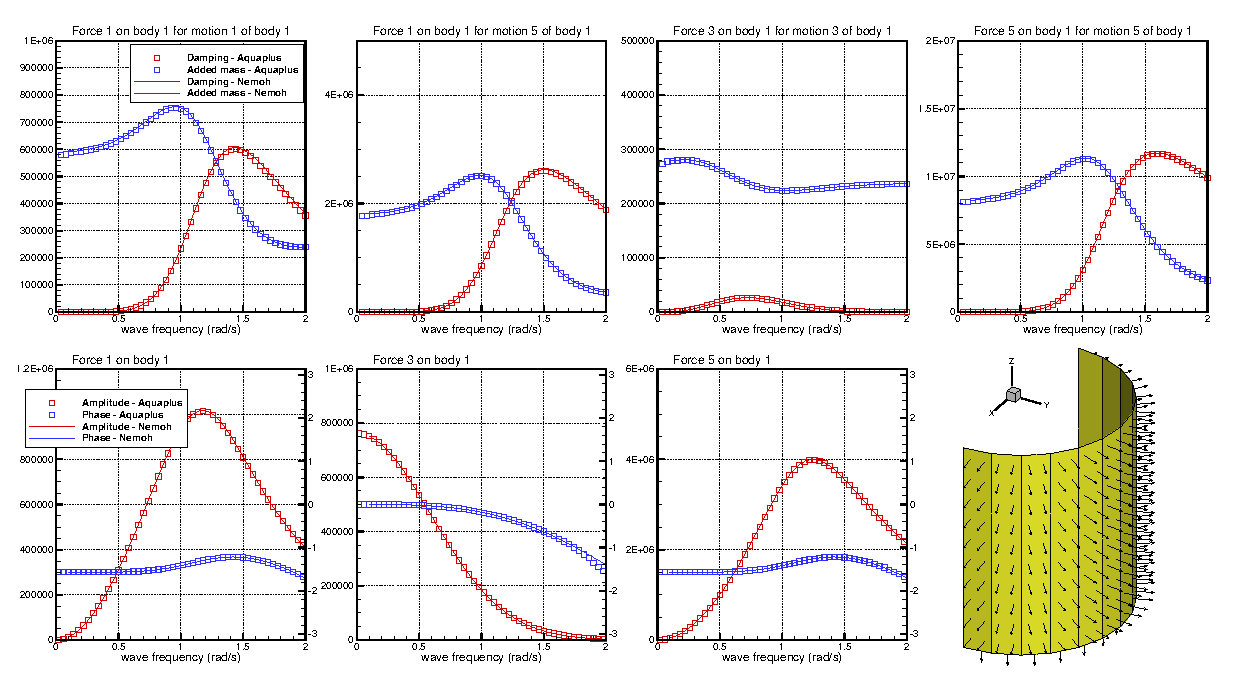
\includegraphics[scale=0.8,trim = 0mm 0mm 0mm 0mm, clip]{figures/Ver_Cylinder.eps}
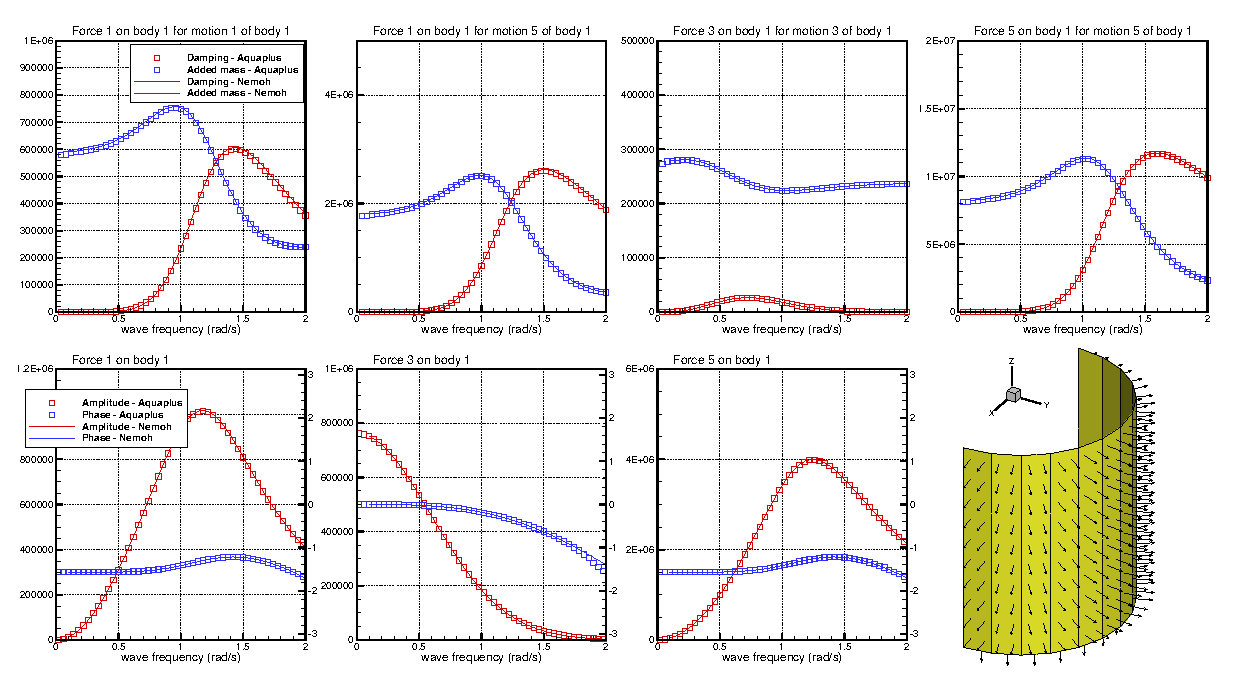
\includegraphics[width=\textwidth,trim = 0mm 0mm 0mm 0mm, clip]{figures/Ver_Cylinder.eps}
\caption{Comparison of the first order results between NEMOH and AQUAPLUS for the test case \textbf{1\_Cylinder}}\label{fig:Cylinder}
\end{figure}
\item \textbf{2\_2Bodies}: half-symmetric body mesh, two different bodies, water depth $20$ m, wave direction $45^{\circ}$. The results are shown in Fig. \ref{fig:2Bodies}.
\begin{figure}[h!t]
\centering
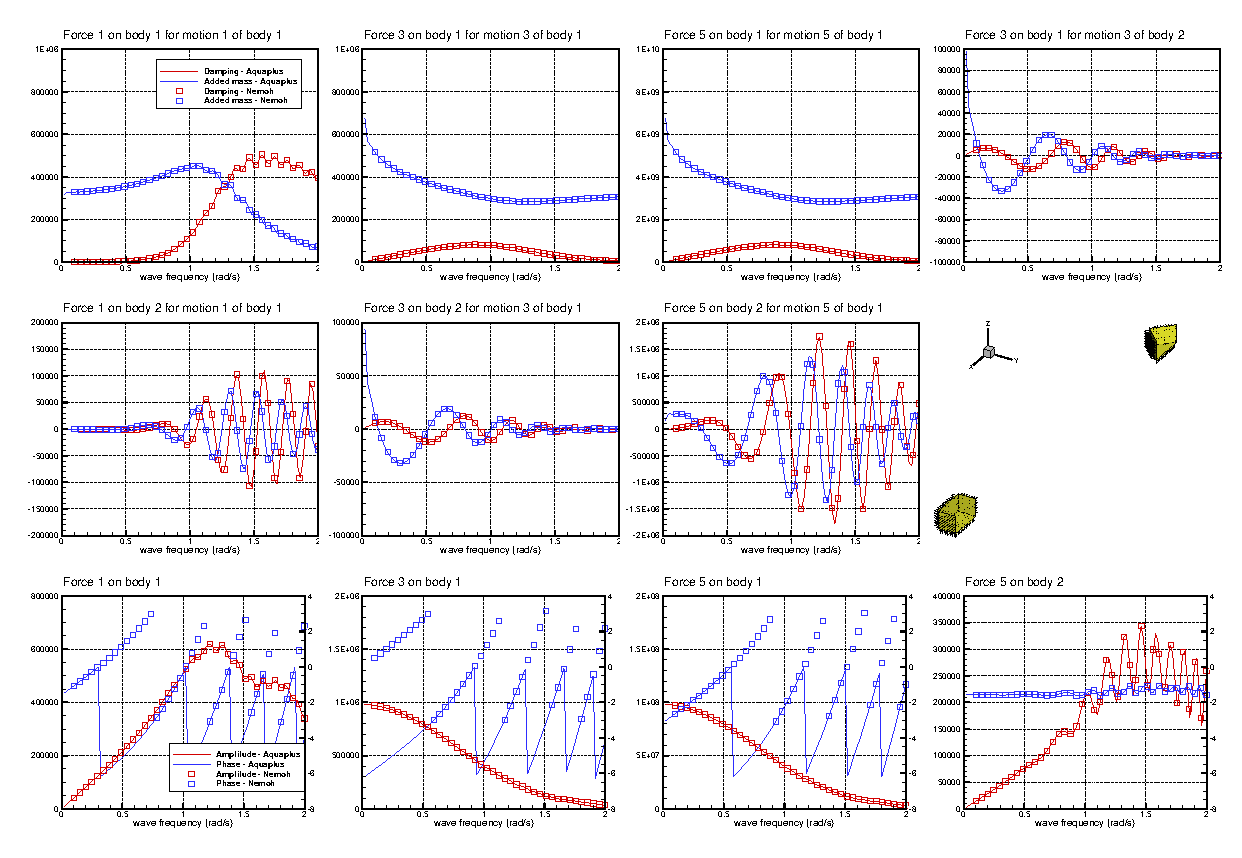
\includegraphics[width=\textwidth,trim = 0mm 0mm 0mm 0mm, clip]{figures/Ver_2Bodies.eps}	
\caption{Comparison of the first order results between NEMOH and AQUAPLUS for the test case \textbf{2\_2Bodies}}\label{fig:2Bodies}
\end{figure}
\item \textbf{3\_Nonsymmetrical}: full non-symmetrical body mesh, deep-water, wave direction $0^{\circ}$. Comparison of NEMOH results against Aquaplus are shown in Fig. \ref{fig:NonSymmetrical}, a slight difference are observed in the results.  Added mass and damping coefficients comparison between NEMOH and HYDROSTAR are shown in Fig. \ref{fig:NonSymmetrical_massdamp} and for the excitation force is in Fig. \ref{fig:NonSymmetrical_excforce}. Good agreement between NEMOH and HYDROSTAR is achieved. 
\begin{figure}[h!t]
\centering
\subfigure{
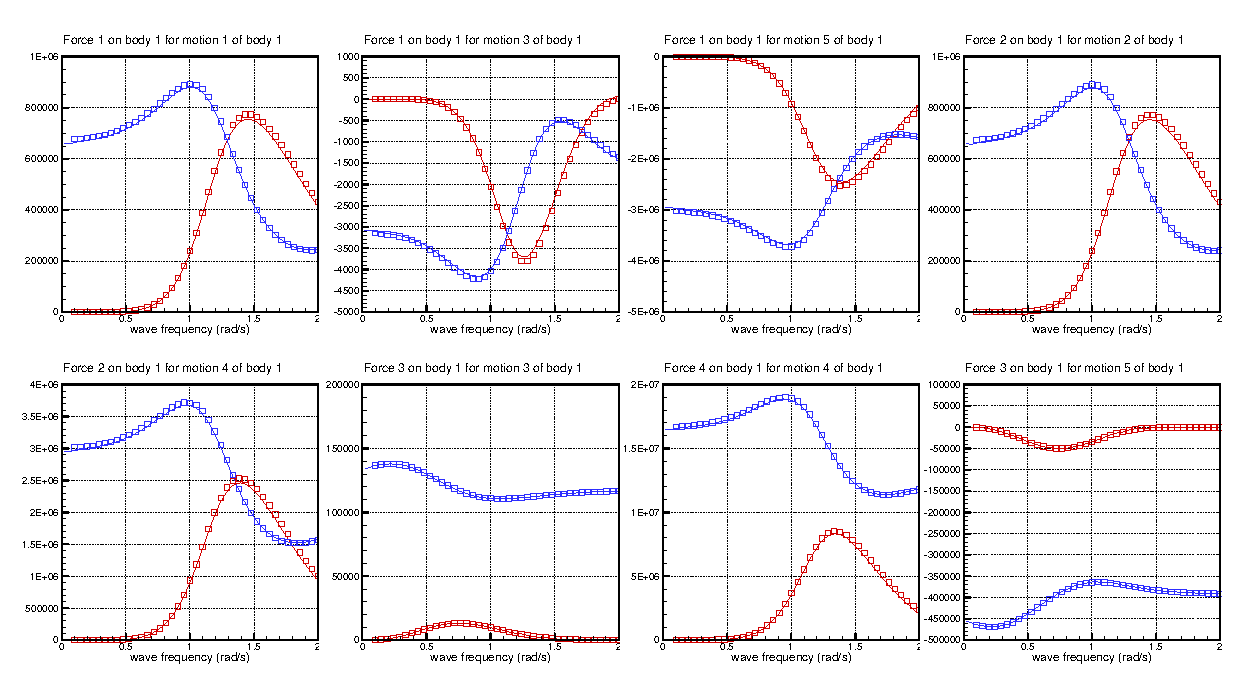
\includegraphics[scale=0.6,trim = 0mm 0mm 0mm 0mm, clip]{figures/Ver_NonSymmetrical_1.eps}	
}
\subfigure{
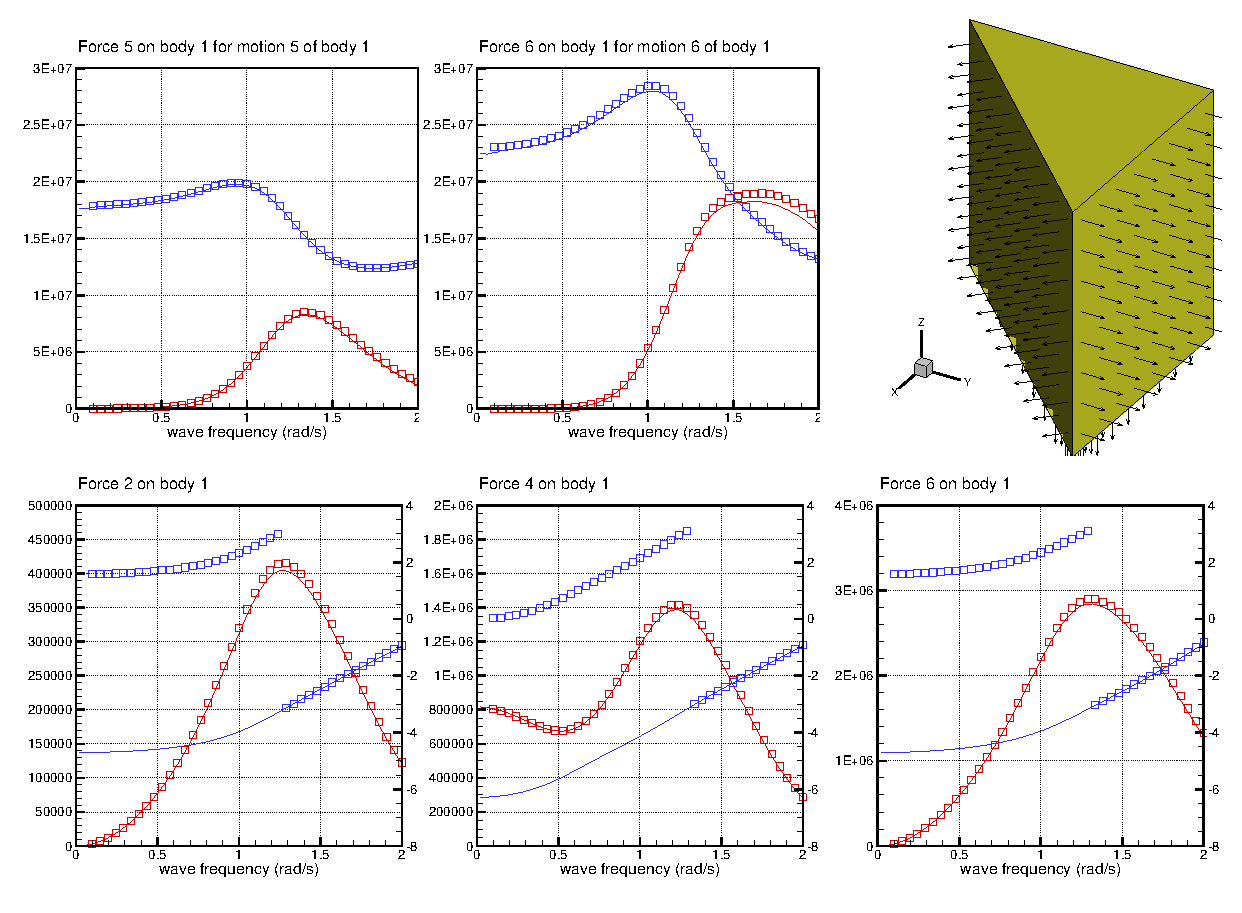
\includegraphics[scale=0.6,trim = 0mm 0mm 0mm 0mm, clip]{figures/Ver_NonSymmetrical_2.eps}	
}
\caption{Comparison of the first order results between NEMOH and AQUAPLUS for the test case \textbf{3\_Nonsymmetrical}}\label{fig:NonSymmetrical}
\end{figure}

\begin{figure}[h!tbp]
\centering
\subfigure[added mass]{
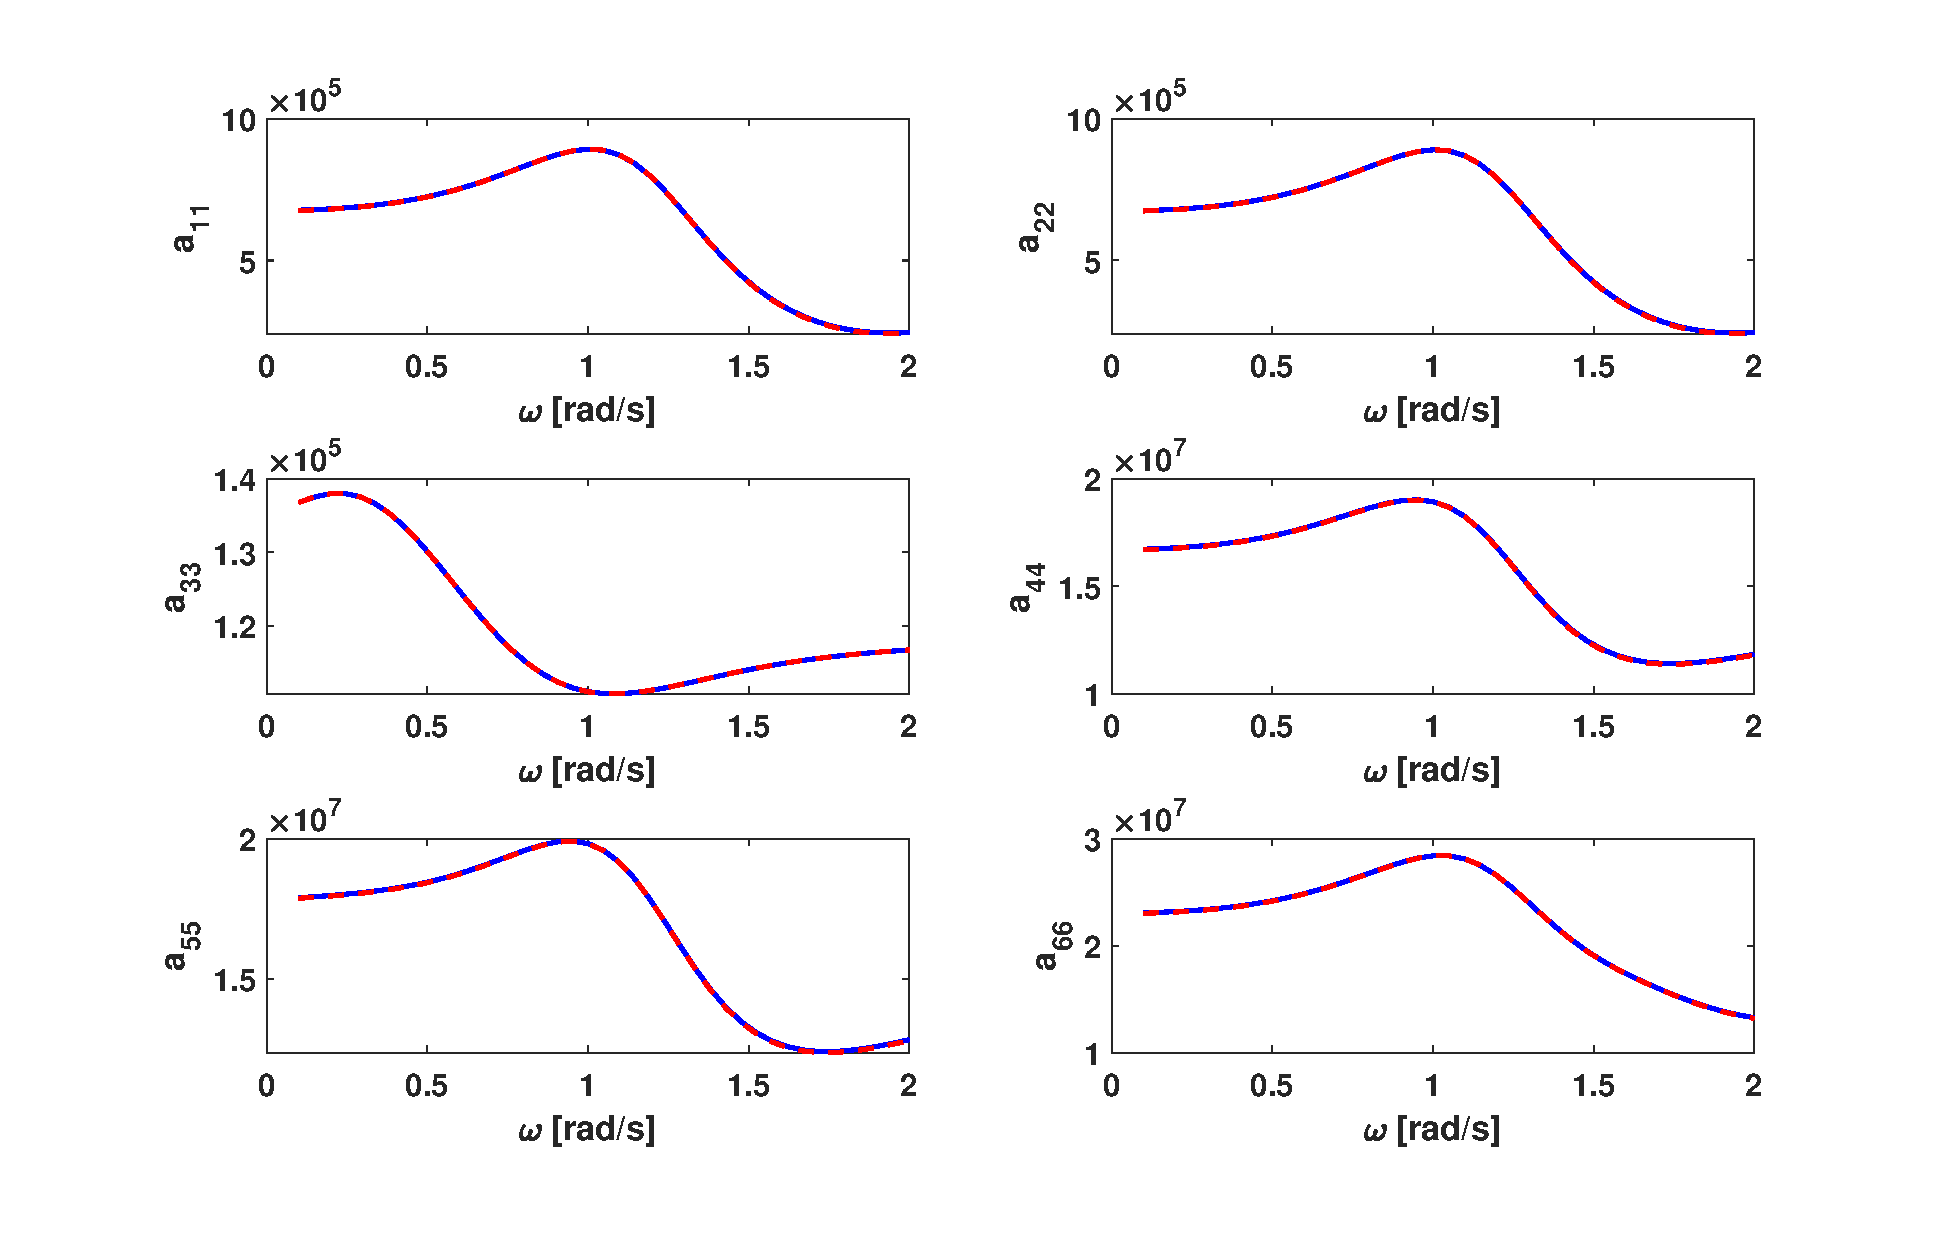
\includegraphics[scale=0.5,trim = 10mm 0mm 30mm 0mm, clip]{figures/Ver_NonSymmetrical_addedmass.eps}	
}
\subfigure[damping coefficients]{
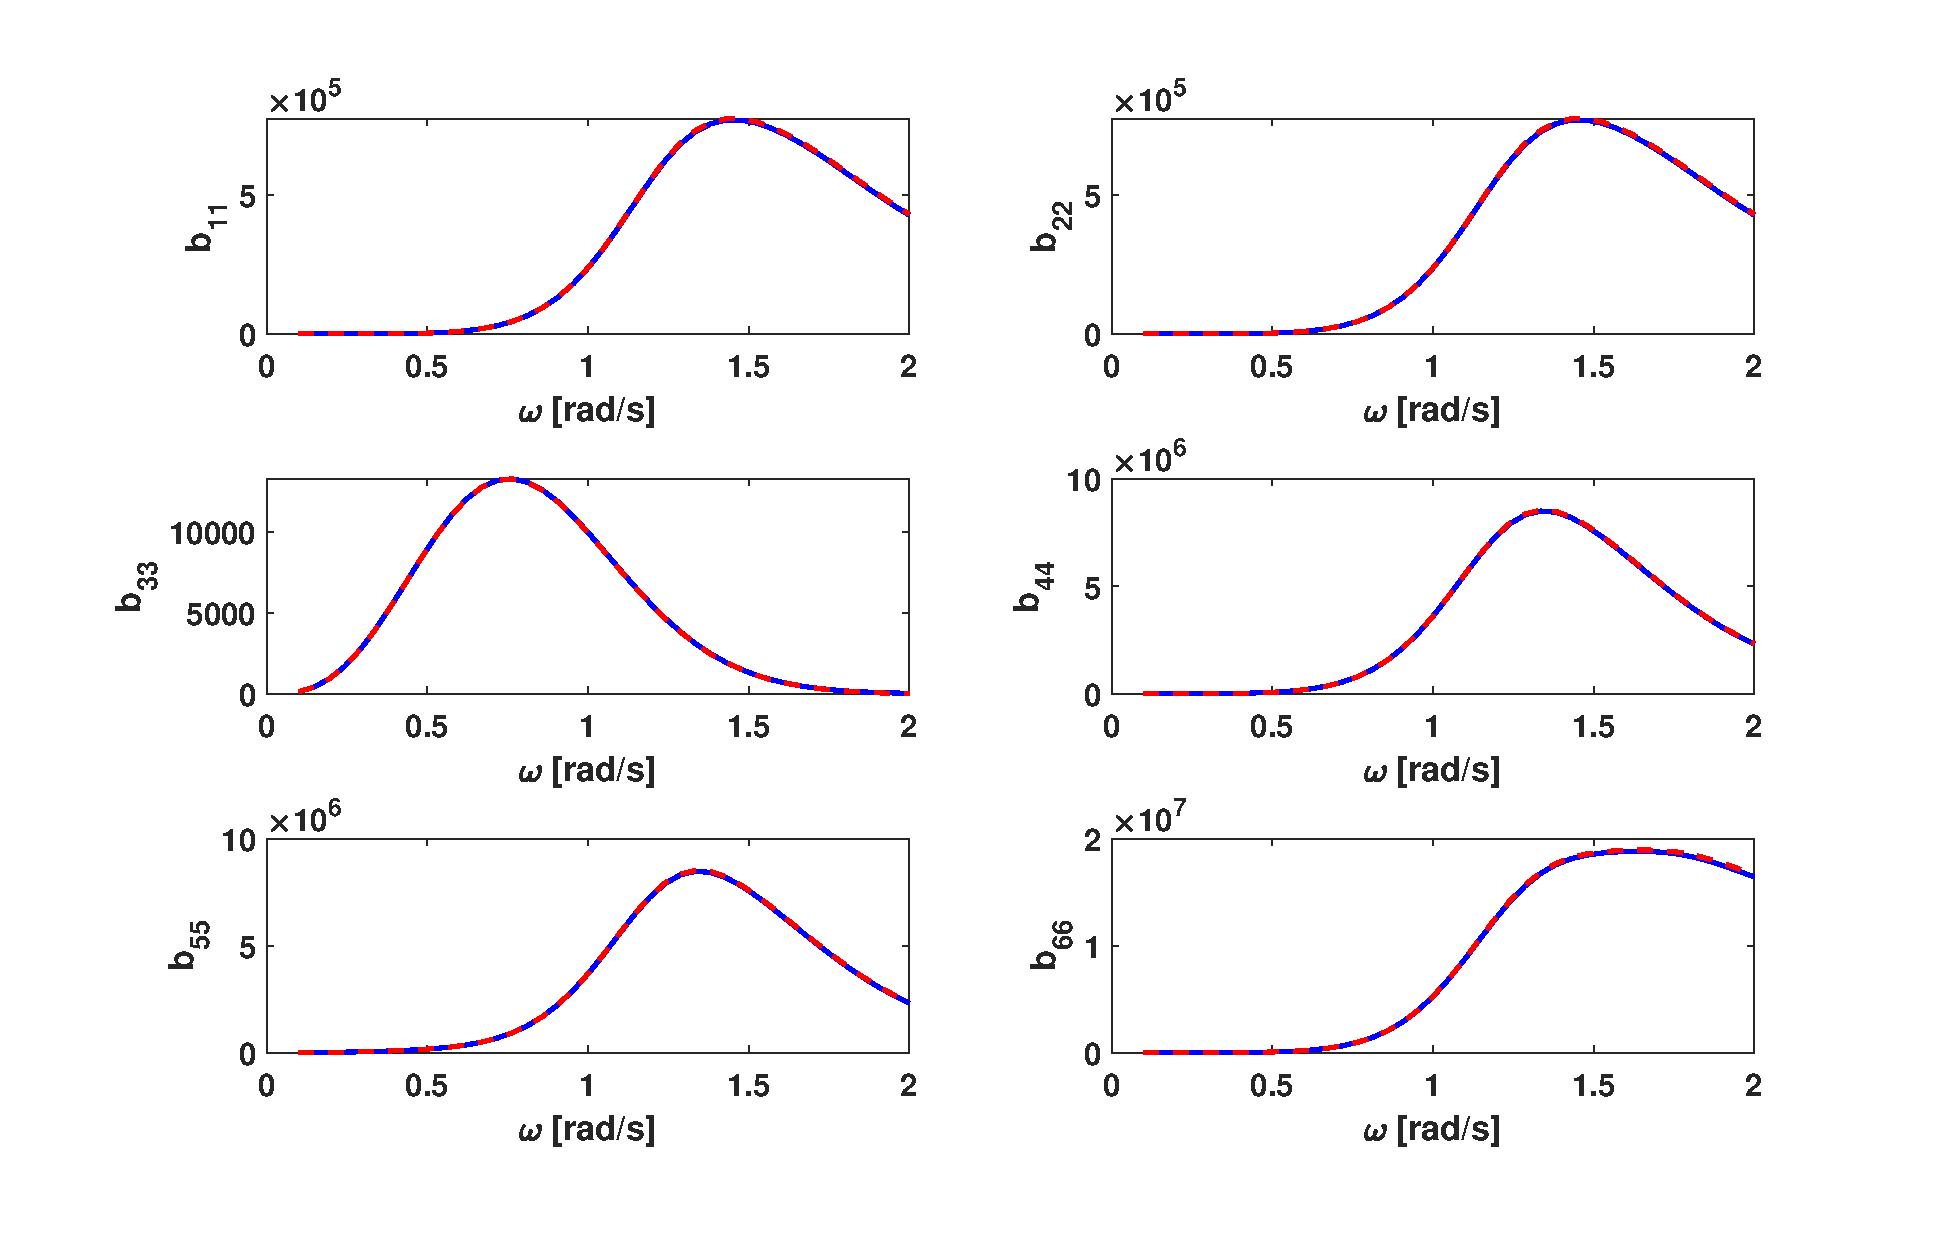
\includegraphics[scale=0.5,trim = 10mm 0mm 30mm 0mm, clip]{figures/Ver_NonSymmetrical_dampcoef.eps}	
}
\caption{Comparison of added mass and damping coefficients between NEMOH, red dashed-line, and HYDROSTAR, blue solid-line, for the test case \textbf{3\_Nonsymmetrical}}\label{fig:NonSymmetrical_massdamp}
\end{figure}

\begin{figure}[h!tbp]
\centering
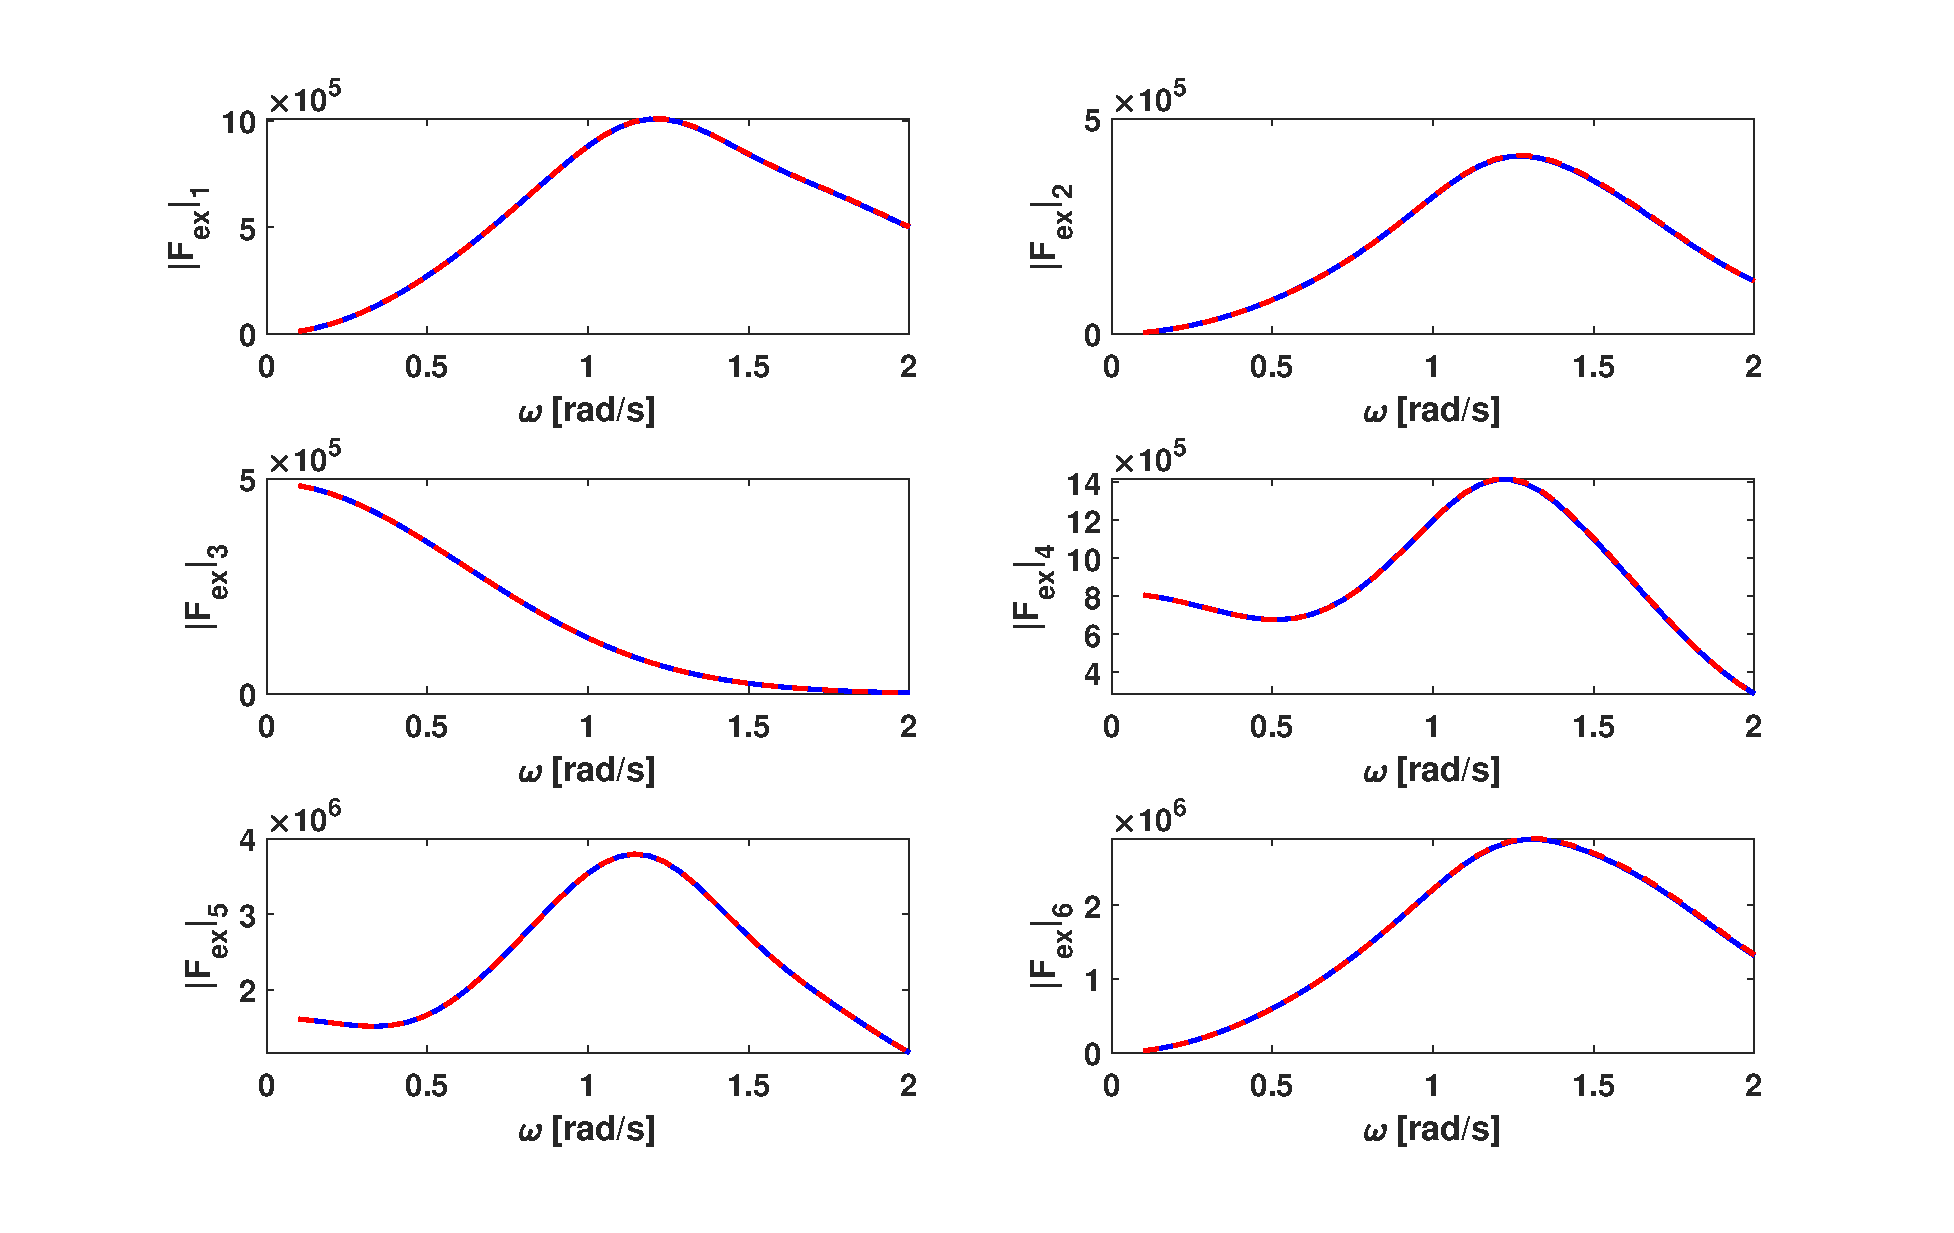
\includegraphics[scale=0.5,trim = 10mm 0mm 30mm 0mm, clip]{figures/Ver_NonSymmetrical_excitationforce.eps}	
\caption{Comparison of excitation force between NEMOH, red dashed-line, and HYDROSTAR, blue solid-line, for the test case \textbf{3\_Nonsymmetrical}}\label{fig:NonSymmetrical_excforce}
\end{figure}

\item \textbf{4\_Postprocessing}: half-symmetric body mesh, water depth $10$ m, wave direction $0^{\circ}$. This test case shows a comparison of the free-surface elevation and the Kochin function. The results are shown in Fig. \ref{fig:PostProcessing}. The phase difference, $\pm \pi/2$, of wave elevation between NEMOH and AQUAPLUS is due to different conventions of the incident potential.

\begin{figure}[h!tbp]
\centering
\subfigure{
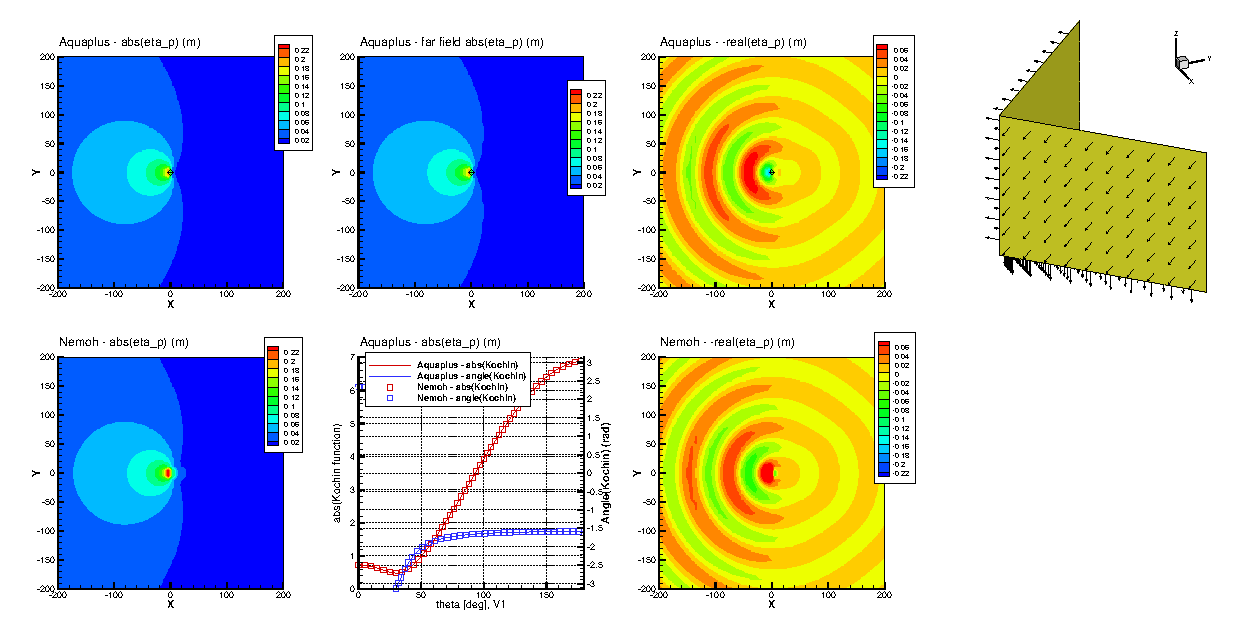
\includegraphics[scale=1,trim = 0mm 0mm 50mm 0mm, clip]{figures/Ver_PostProcessing.eps}	
}\\
\subfigure{
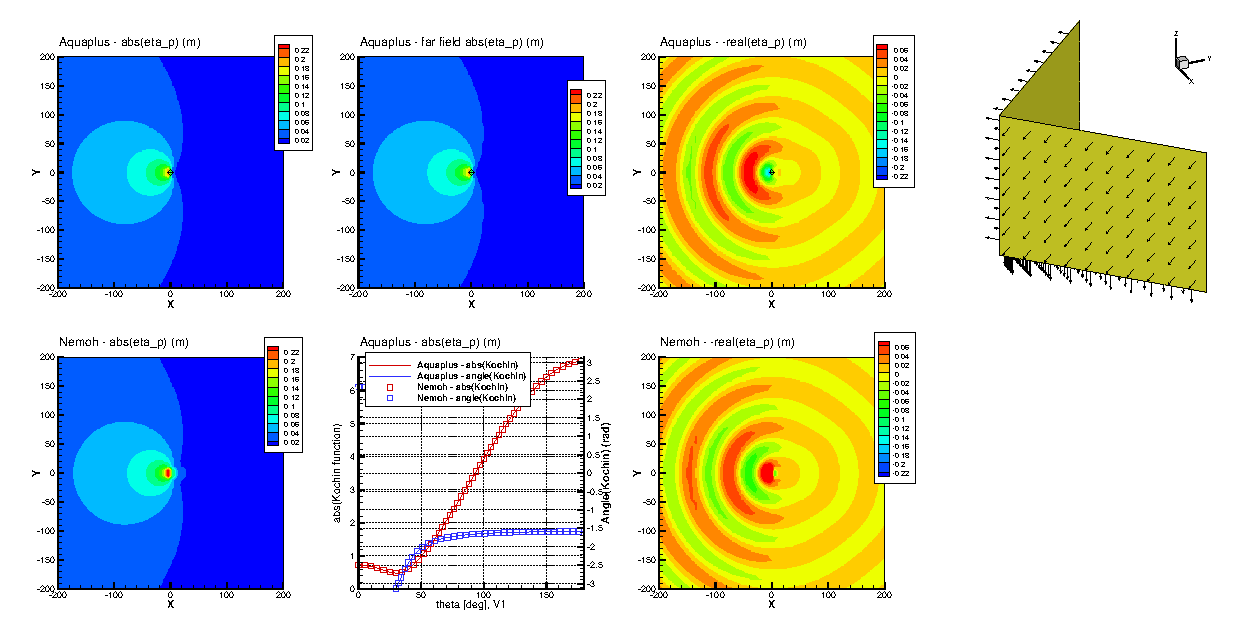
\includegraphics[scale=1,trim = 160mm 50mm 0mm 0mm, clip]{figures/Ver_PostProcessing.eps}	
}
%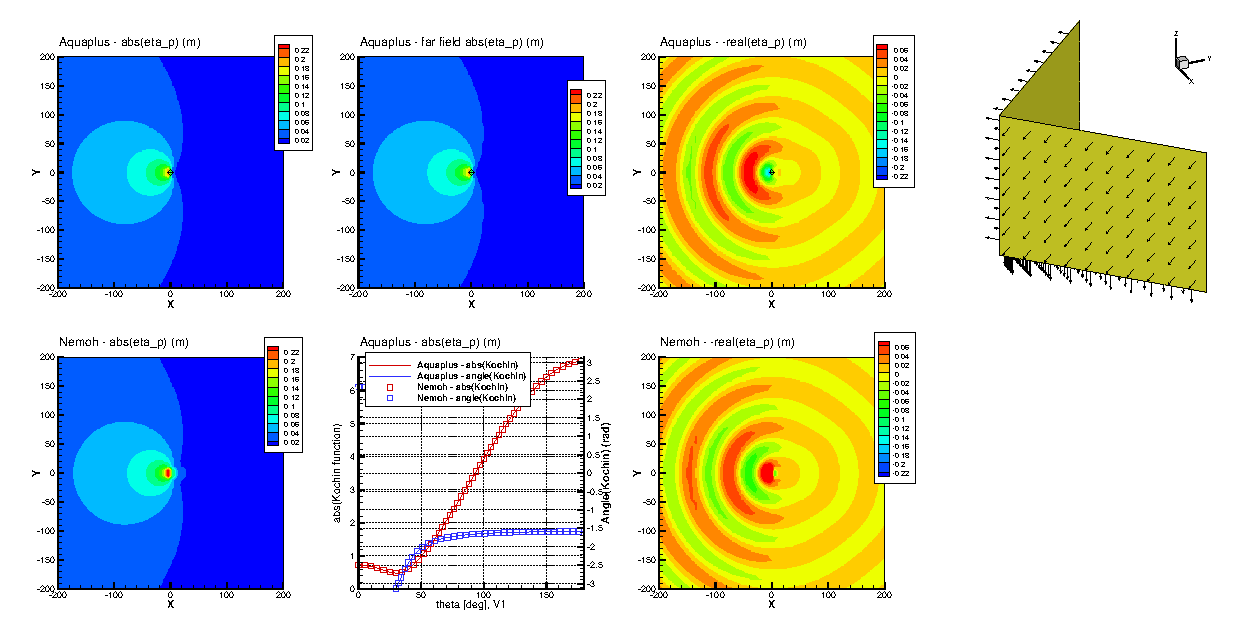
\includegraphics[width=\linewidth]{figures/Ver_PostProcessing.eps}	
\caption{Comparison of the diffracted wave elevation, the diffraction Kochin function between NEMOH and AQUAPLUS, test case \textbf{4\_Postprocessing}}\label{fig:PostProcessing}
\end{figure}

\item \textbf{5\_QuickTest} shows a quantitative comparison of force and free-surface for the first-frequency diffraction problem. The comparison results are shown in the command window for all the test cases inside the directory \texttt{5\_QuickTest}.

\item \textbf{6\_box\_coarsemesh} is showing the procedure for running the code starting with the executable \textbf{\texttt{mesh}} with a coarse description mesh file, \texttt{meshbox}. No reference data is given in this test case.

\item \textbf{7\_Solvers\_Check\_OC3} is testing the performance of the three difference linear solvers, Gauss elimination, LU decomposition and GMRES. Reference logfiles reporting the computational time of the solvers are provided.

\item \textbf{8a\_Cylinder\_irregfreq} shows the results with and without irregular frequencies removal (IRR) method. The results are verified against HYDROSTAR with IRR and shown in Fig. \ref{fig:Cylinder_IRR_addedmass_dampcoef} for the added mass and damping coefficients and in Fig. \ref{fig:Cylinder_IRR_excforce} for the excitation forces. The mesh used was obtained using GMSH \cite{gmsh} and is shown in Fig. \ref{fig:meshesCylinder}.

\begin{figure}[h!tbp]
\centering
%\subfigure{
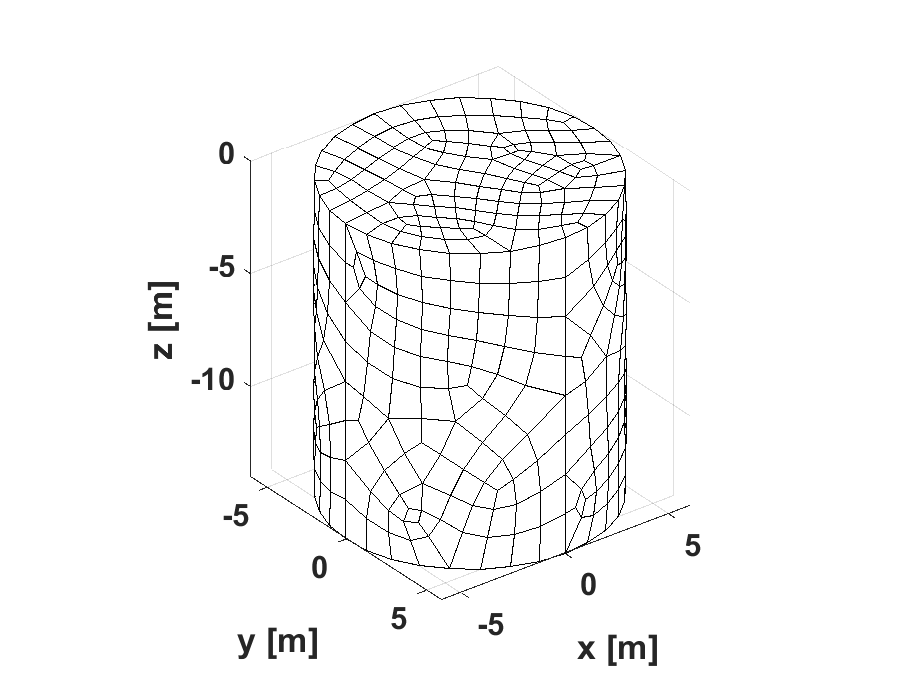
\includegraphics[scale=0.5,trim = 0mm 0mm 0mm 0mm, clip]{figures/Cylinder/mesh.eps}	
%}
\caption{Body boundary mesh for the Cylinder used for test case \textbf{8a\_Cylinder\_irregfreq} and \textbf{8b\_QTF\_Cylinder}.}\label{fig:meshesCylinder}
\end{figure}

\begin{figure}[h!tbp]
\centering
\subfigure[added mass]{
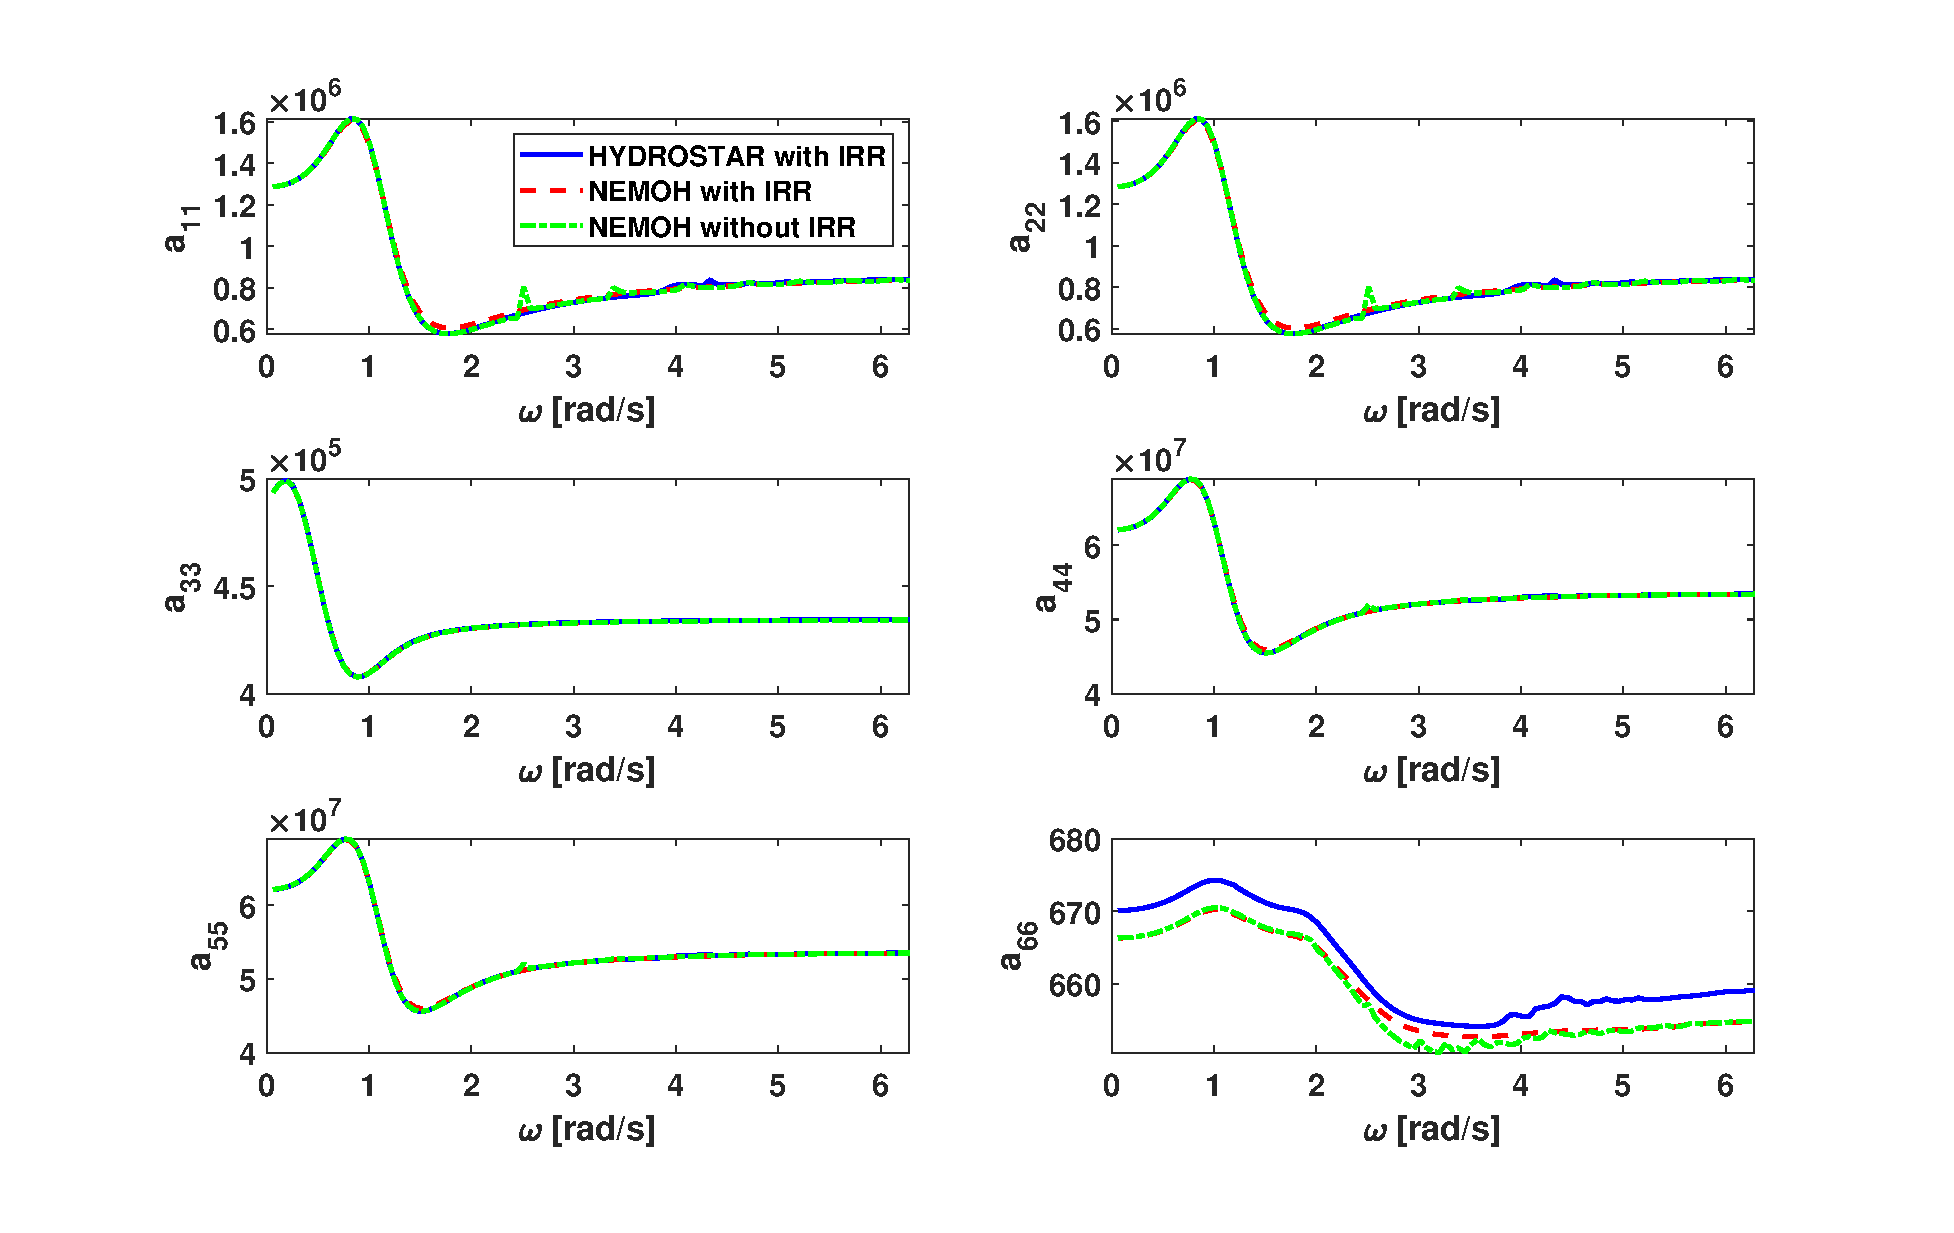
\includegraphics[scale=0.5,trim = 10mm 0mm 30mm 0mm, clip]{figures/Cylinder/addedmass.eps}	
}
\subfigure[damping coefficients]{
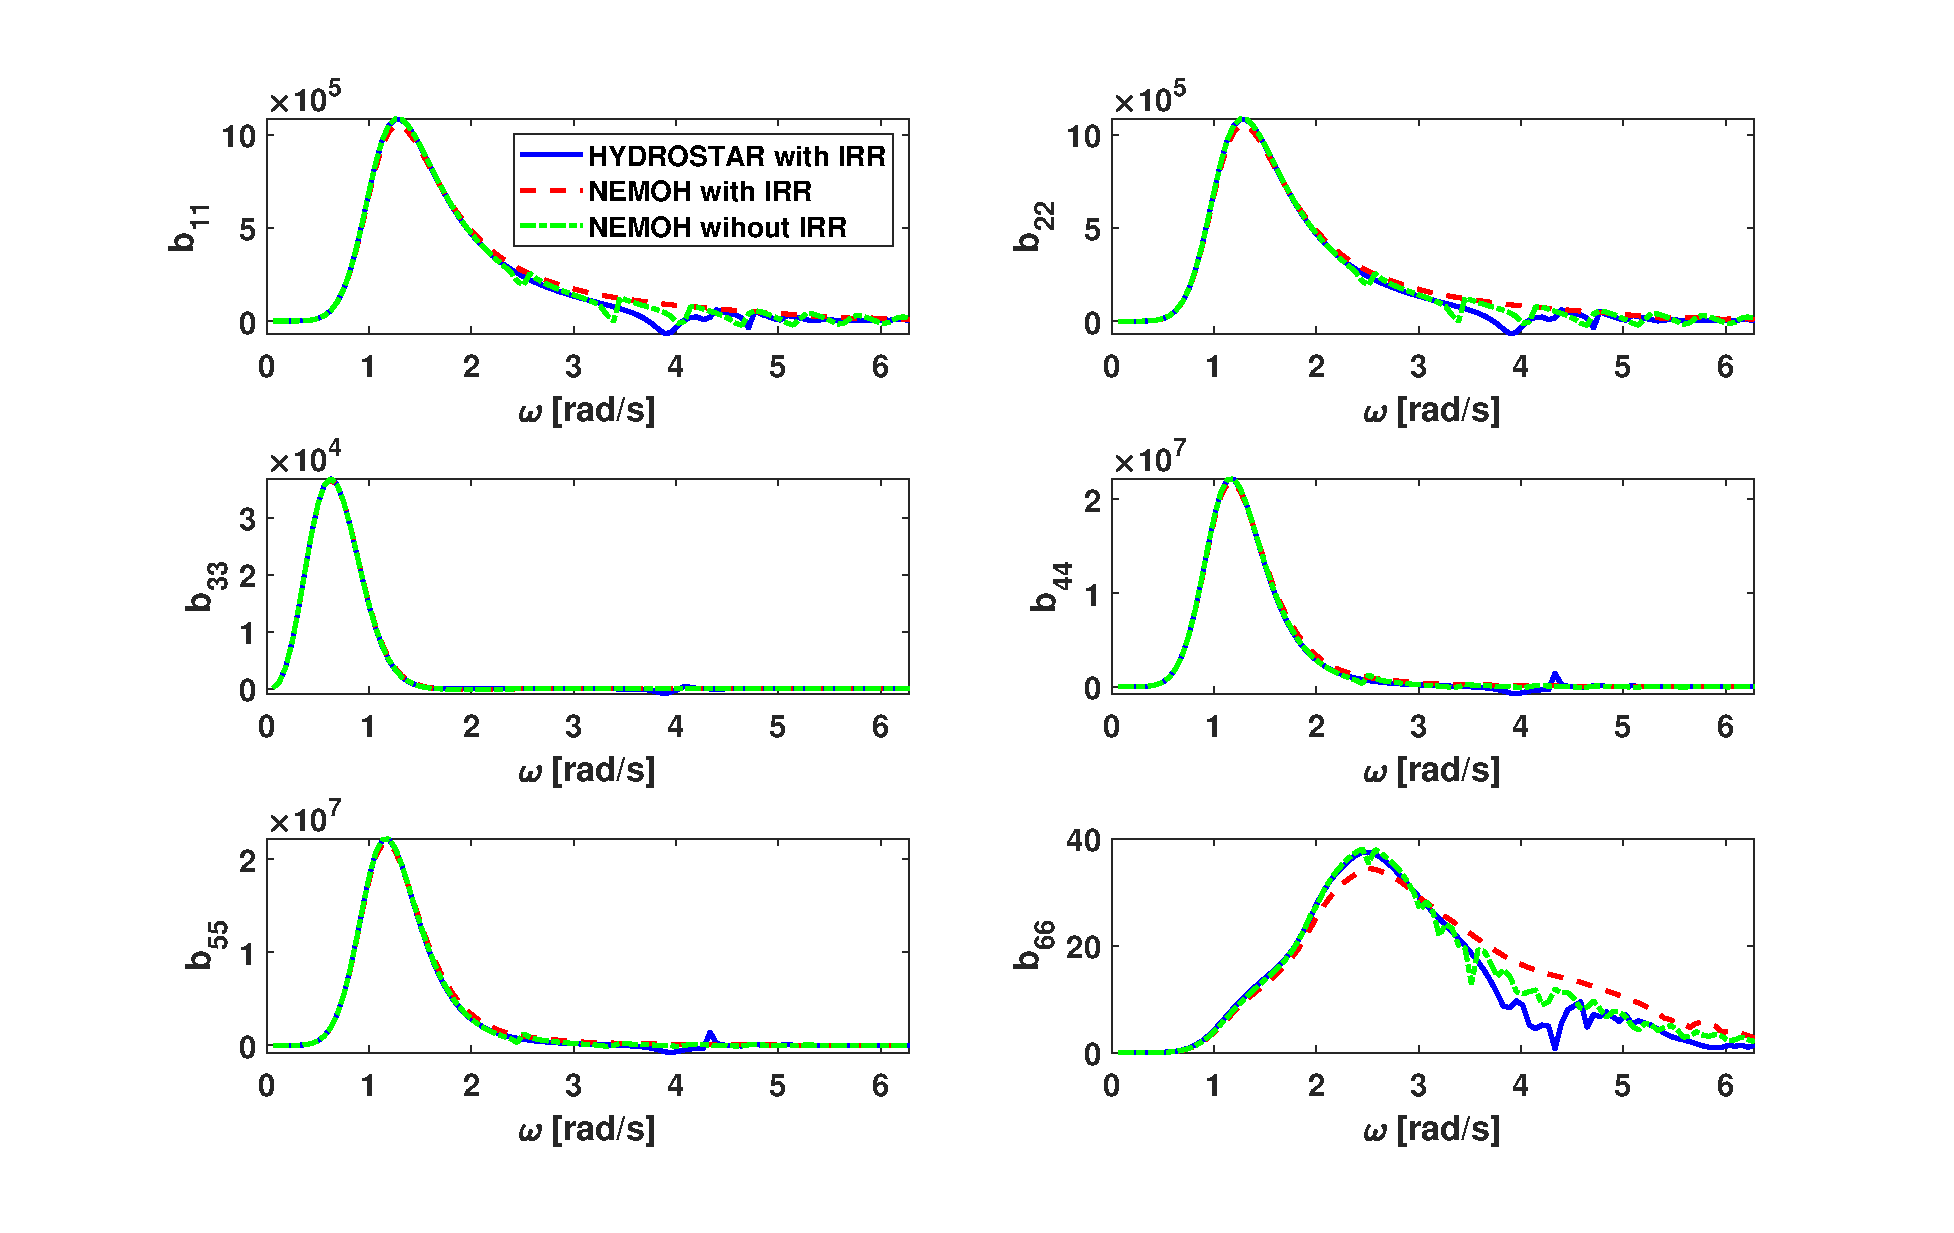
\includegraphics[scale=0.5,trim = 10mm 0mm 30mm 0mm, clip]{figures/Cylinder/dampcoef.eps}	
}
\caption{Comparison of added mass and damping coefficients between NEMOH without irregular frequencies removal (IRR), green dash-dotted line, NEMOH with IRR, red dashed-line and HYDROSTAR with IRR, blue solid-line, for the test-case \textbf{8a\_Cylinder\_irregfreq}}\label{fig:Cylinder_IRR_addedmass_dampcoef}
\end{figure}

\begin{figure}[h!tbp]
\centering

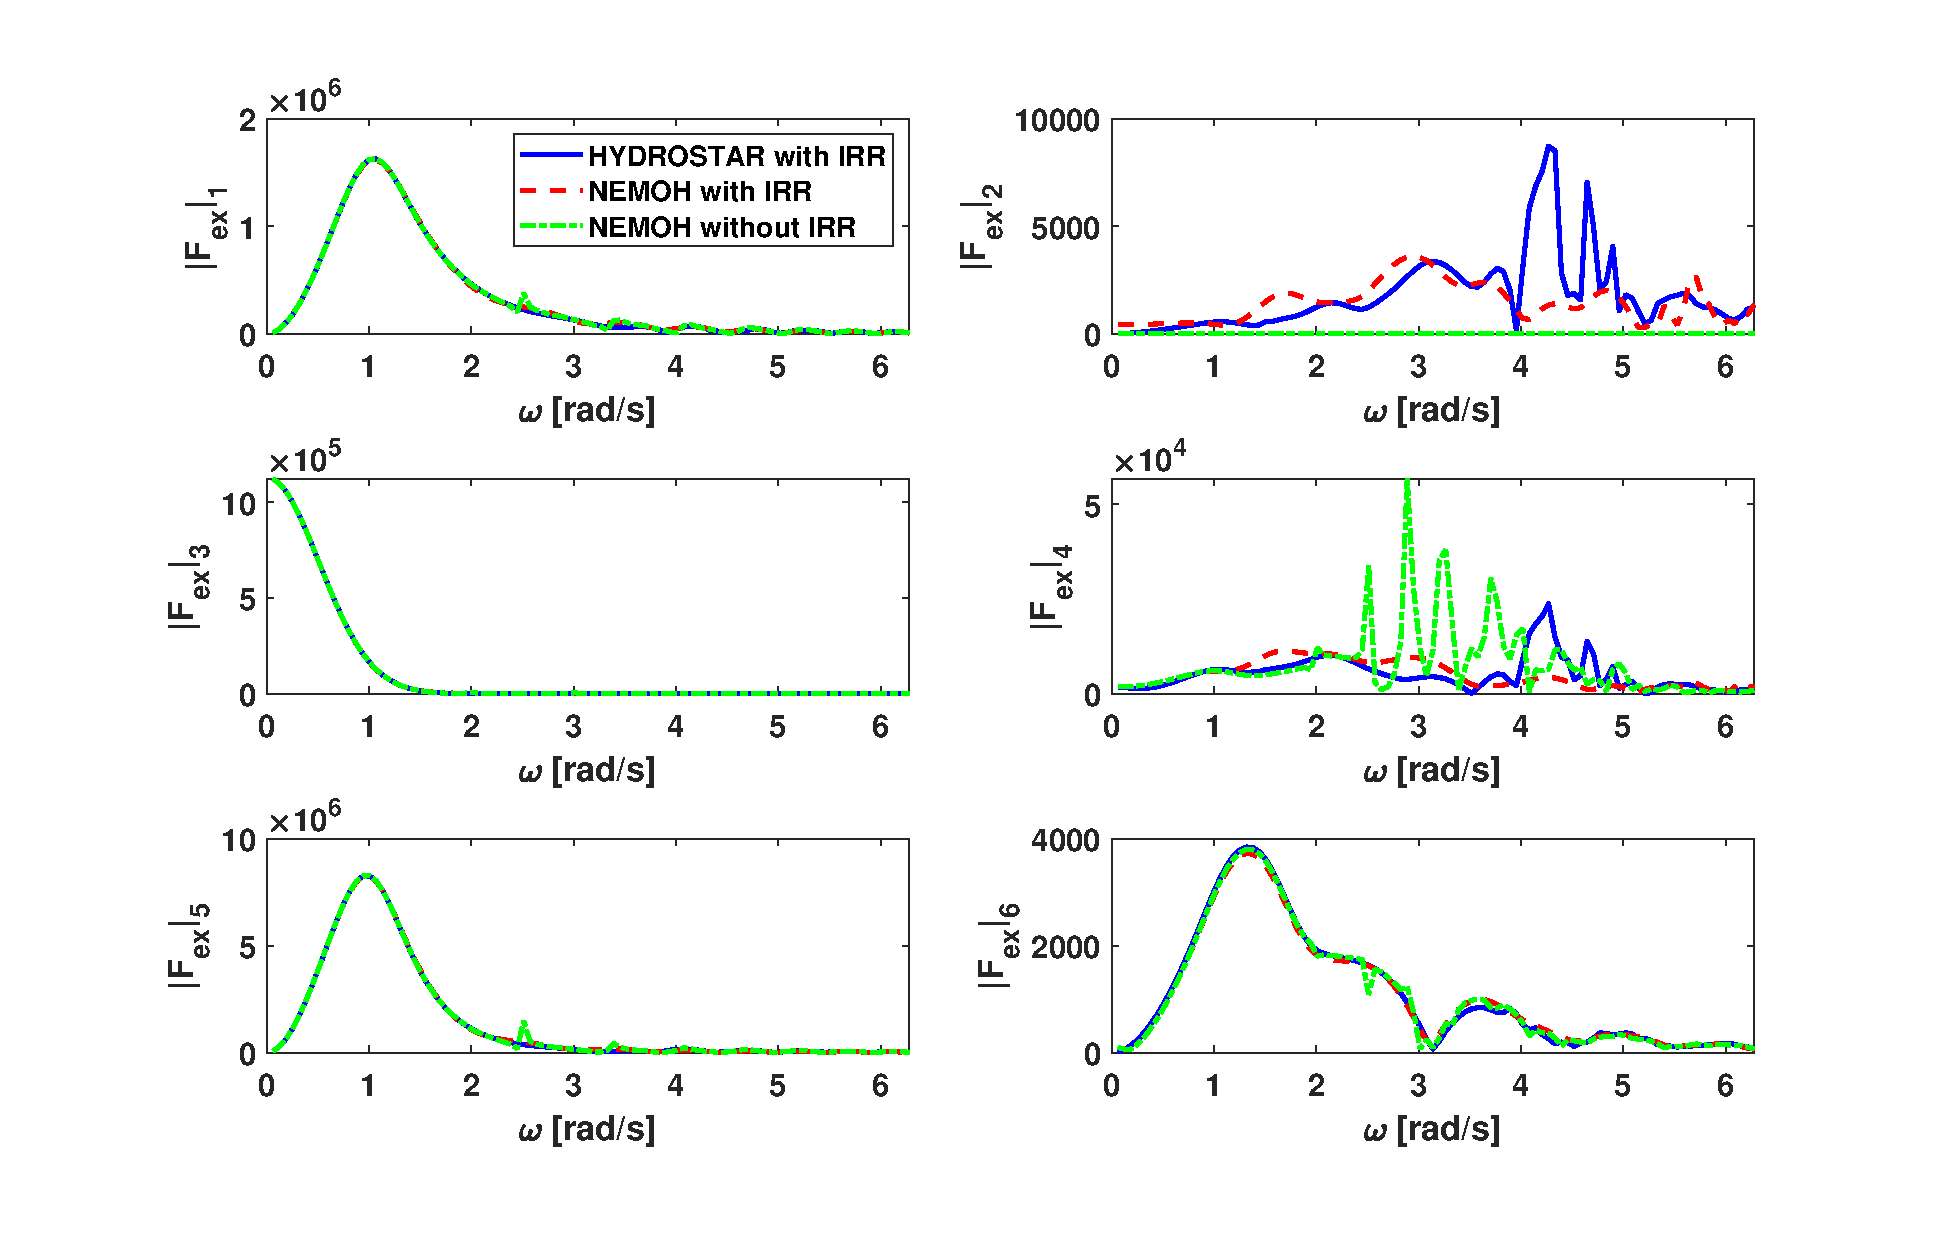
\includegraphics[scale=0.5,trim = 10mm 0mm 30mm 0mm, clip]{figures/Cylinder/excForce.eps}	

\caption{Comparison of excitation force between NEMOH without irregular frequencies removal (IRR), green dash-dotted line, NEMOH with IRR, red dashed-line and HYDROSTAR with IRR, blue solid-line, for the test-case 8a\_Cylinder\_irregfreq}\label{fig:Cylinder_IRR_excforce}
\end{figure}

\end{itemize}

\FloatBarrier

The following test cases are provided for the QTF verification with HYDROSTAR software \cite{HYDROSTAR}.

\begin{itemize}
\item \textbf{8b\_QTF\_Cylinder}: full body mesh with lid panels, CoG $(0,0,0)$, deep water, wave direction $0^{\circ}$, the difference-frequency QTF DUOK+HASBO. The results are shown in the density plot, Fig. \ref{fig:QTFM_Cylinder}, and in the off-diagonal line plot, Fig. \ref{fig:QTFM_diag_Cylinder}. The mesh used was obtained using GMSH \cite{gmsh} and is shown in Fig. \ref{fig:meshesCylinder}.

\begin{figure}[h!tbp]
	\centering
\subfigure{
	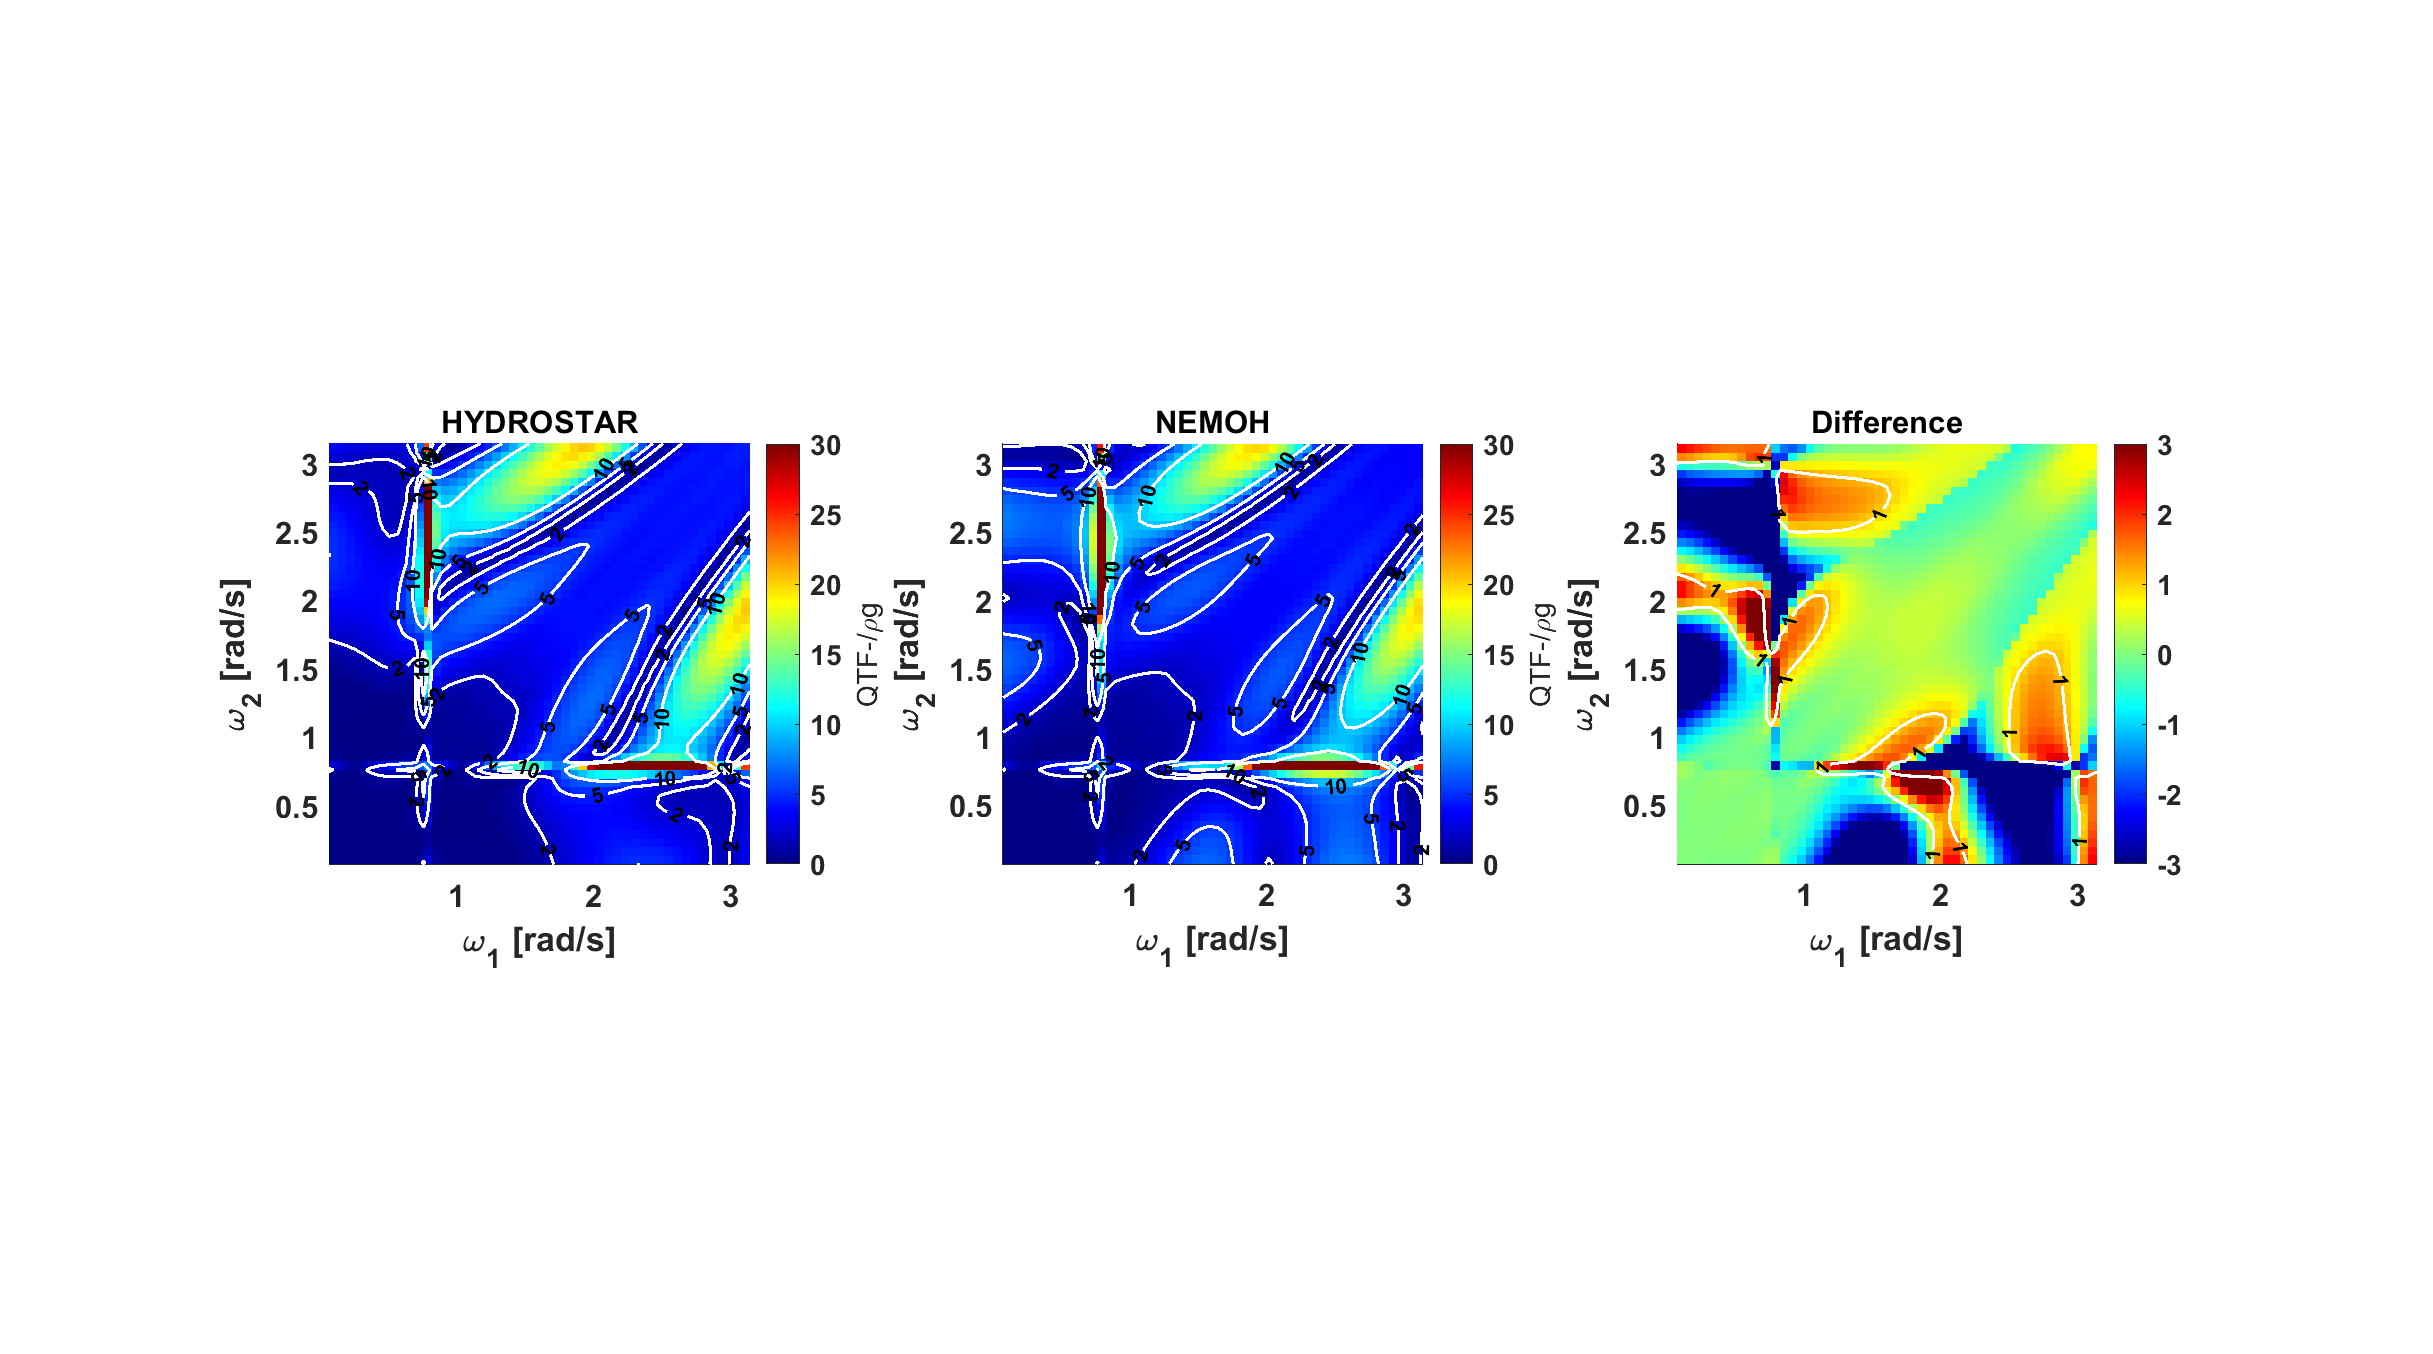
\includegraphics[scale=0.4,trim = 20mm 72mm 25mm 59mm, clip]{figures/Cylinder/QTFsurge.eps}	
}
\subfigure{
	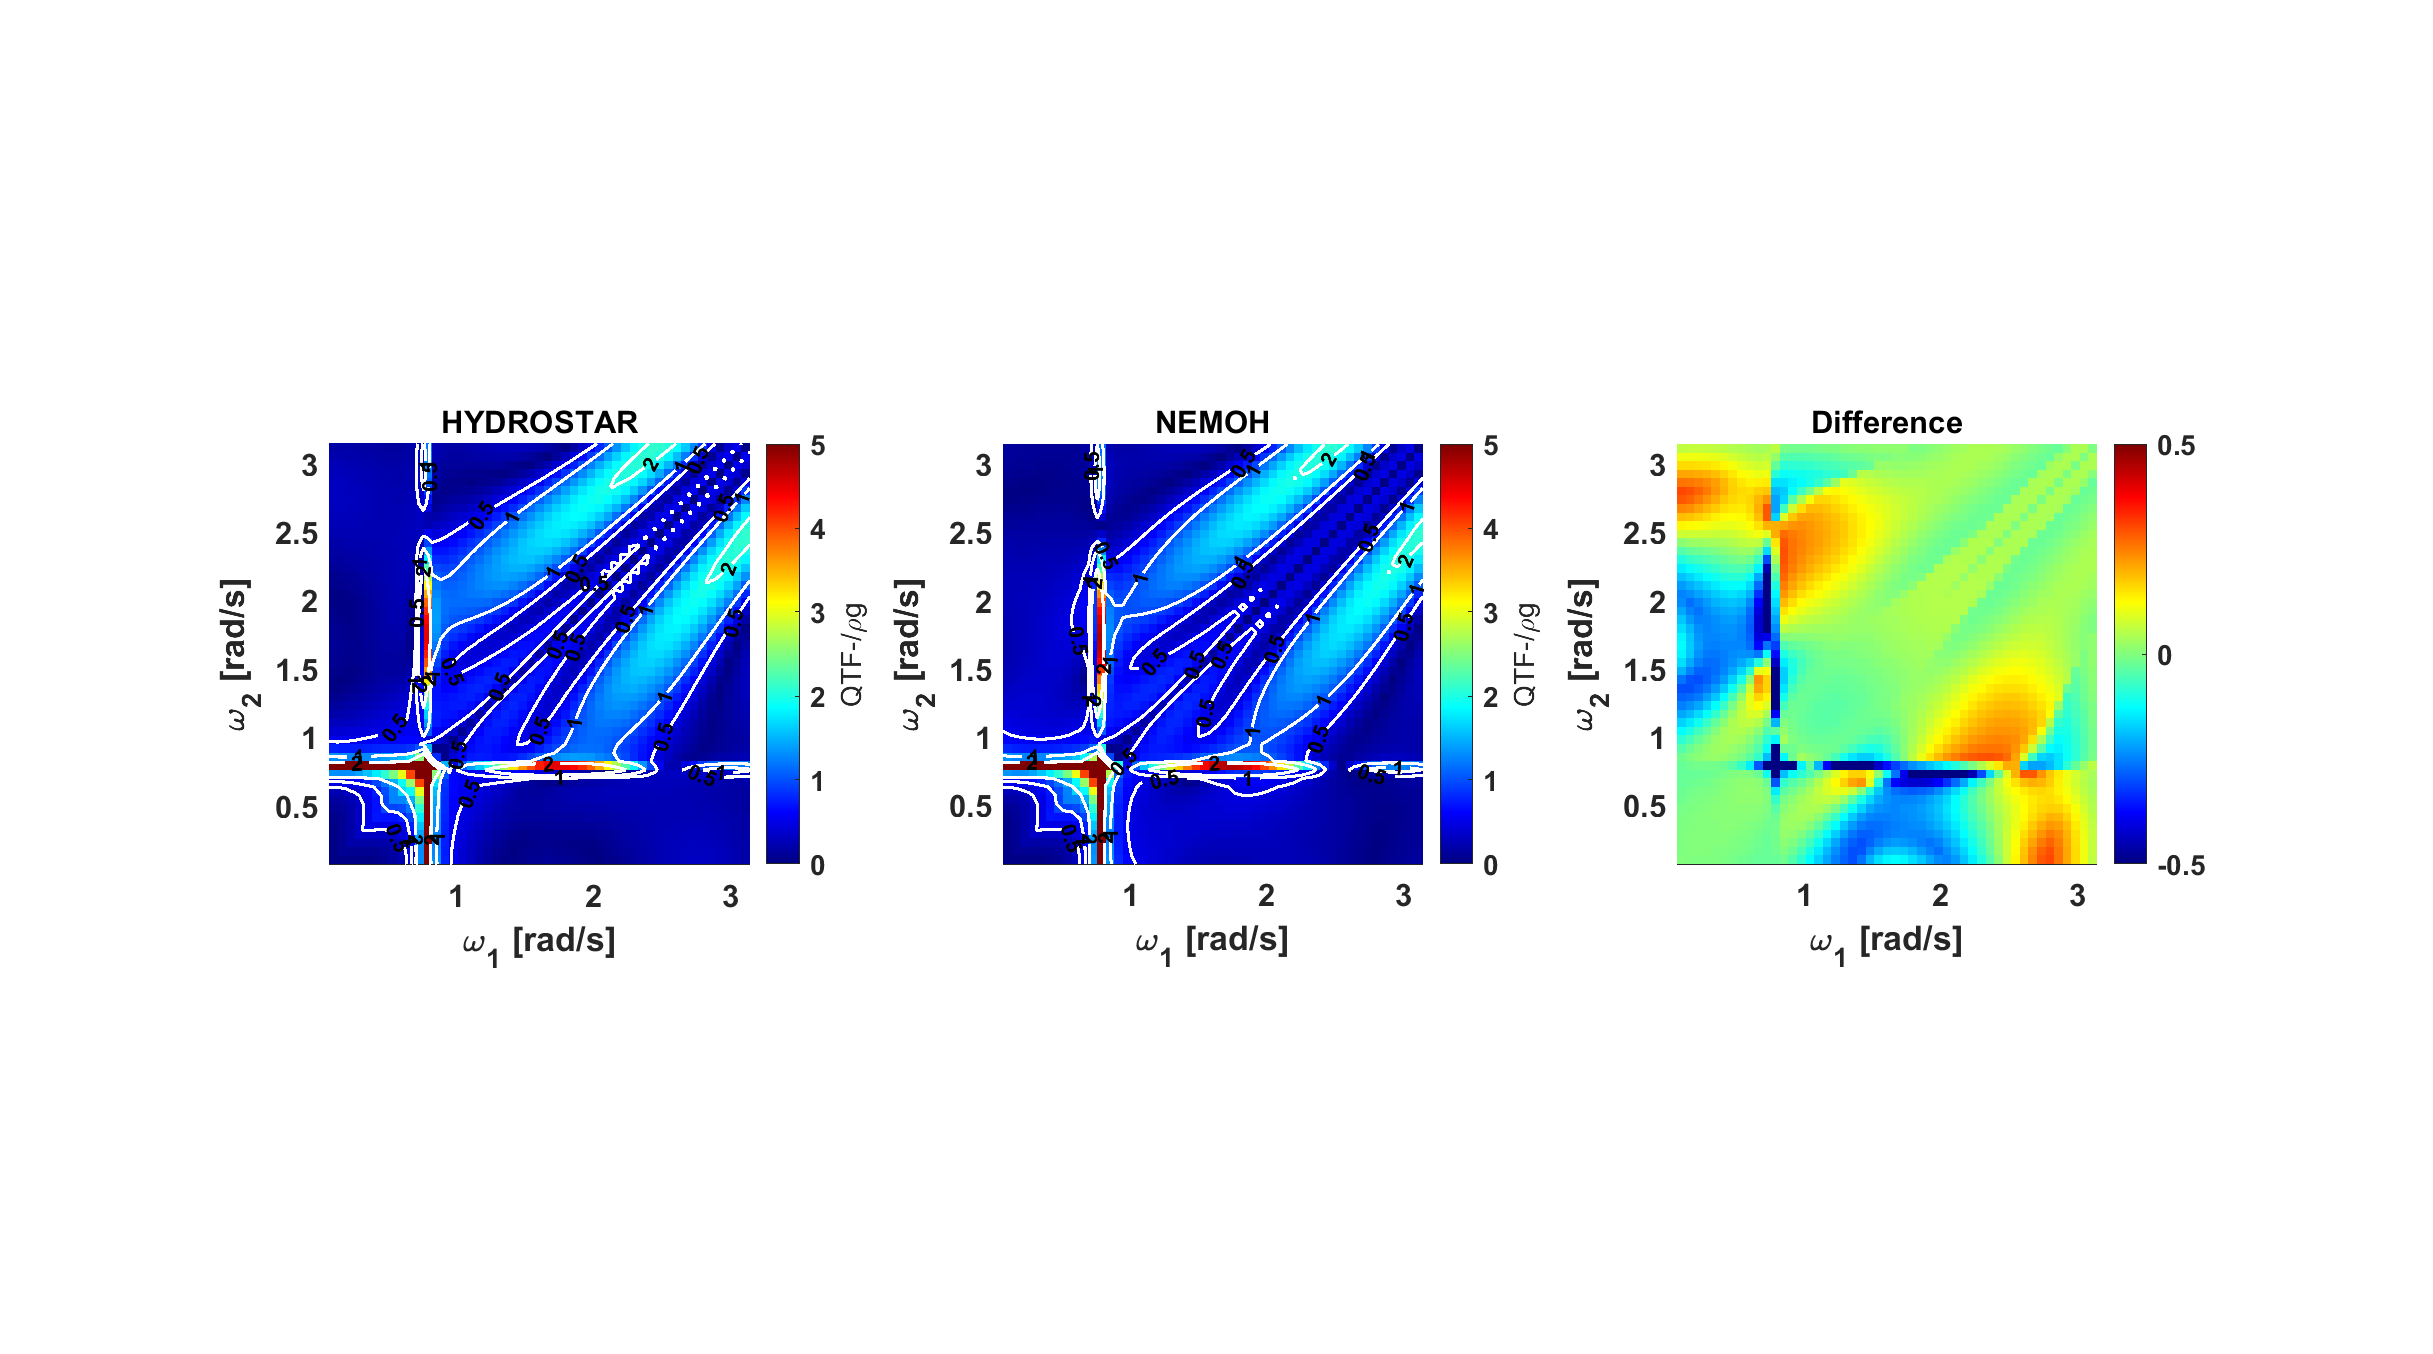
\includegraphics[scale=0.4,trim = 20mm 72mm 20mm 71mm, clip]{figures/Cylinder/QTFheave.eps}	
}
\subfigure{
	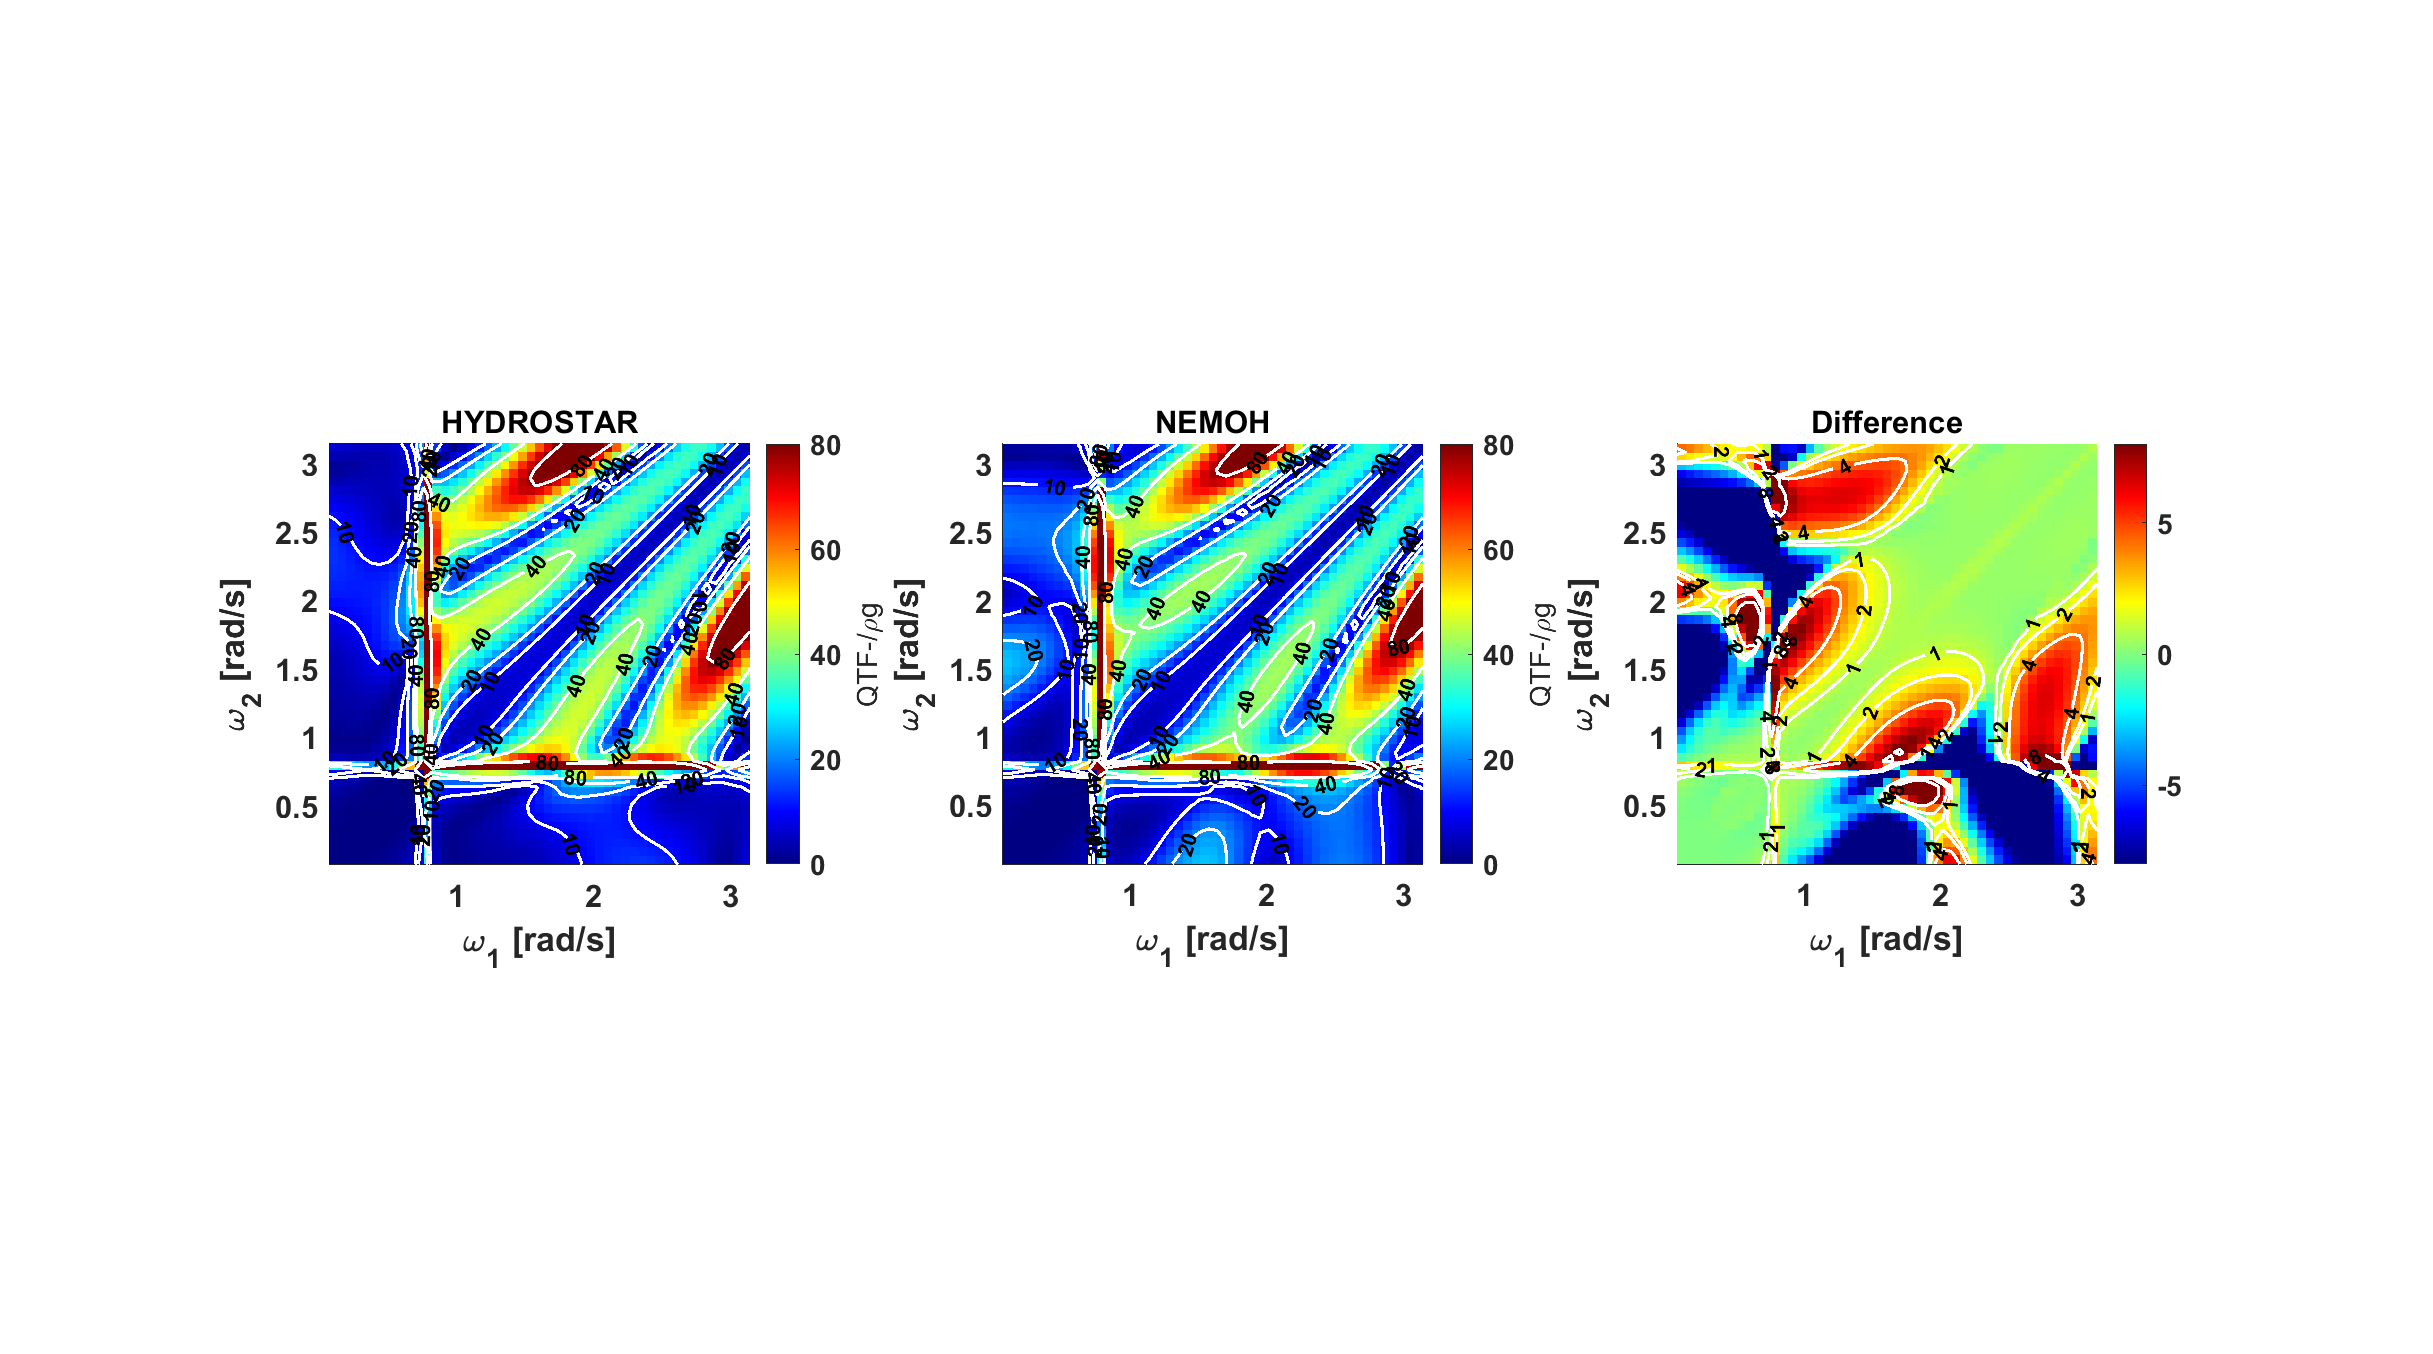
\includegraphics[scale=0.4,trim = 20mm 62mm 20mm 71mm, clip]{figures/Cylinder/QTFpitch.eps}	
}
	\caption{Density plots of the normalized surge difference frequency QTF magnitude (without the free-surface integrals) for the floating Cylinder (test case \textbf{8b\_QTF\_Cylinder}); on the top, middle and bottom rows are for surge, heave and pitch, respectively. HYDROSTAR results are on the left column, NEMOH results are on the middle column and the difference on the right column.}\label{fig:QTFM_Cylinder}
\end{figure}

\begin{figure}[h!tbp]
	\centering
\subfigure{
	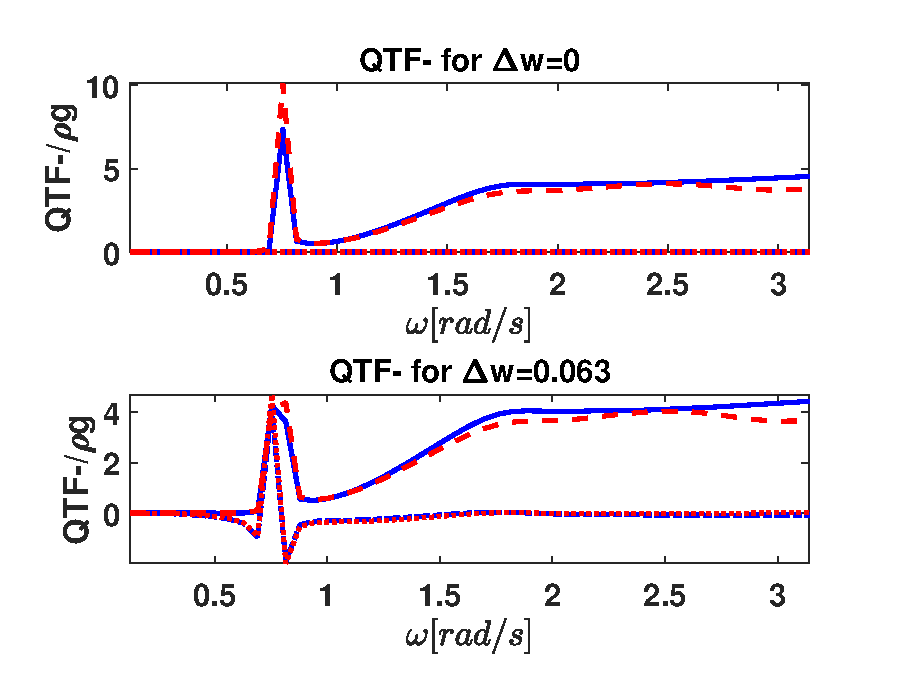
\includegraphics[scale=0.5,trim = 5mm 10mm 5mm 56mm, clip]{figures/Cylinder/QTFsurge_diag.eps}	
}
\subfigure{
	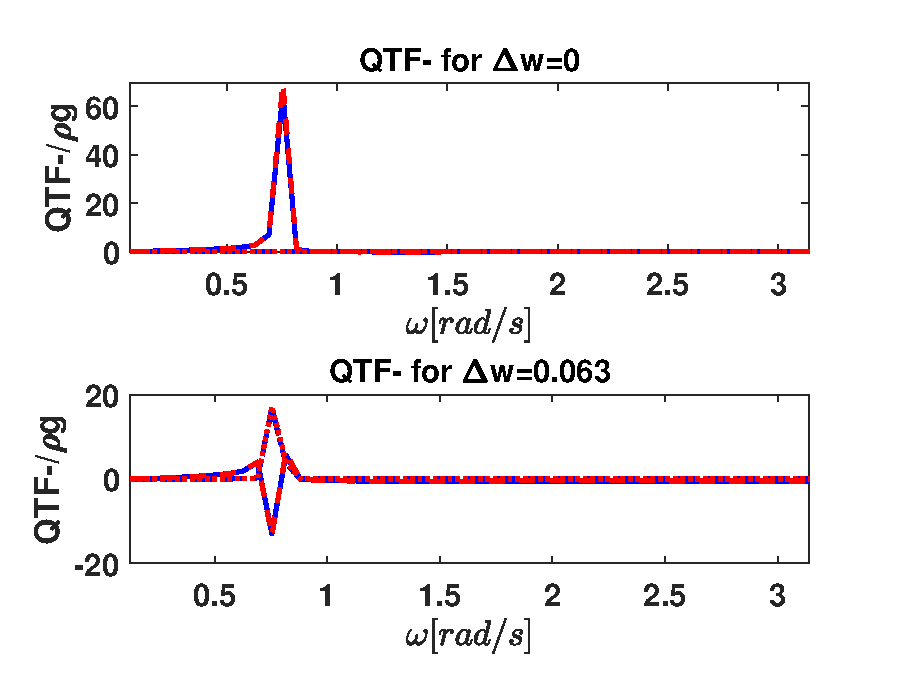
\includegraphics[scale=0.5,trim = 5mm 10mm 5mm 56mm, clip]{figures/Cylinder/QTFheave_diag.eps}	
}
\subfigure{
	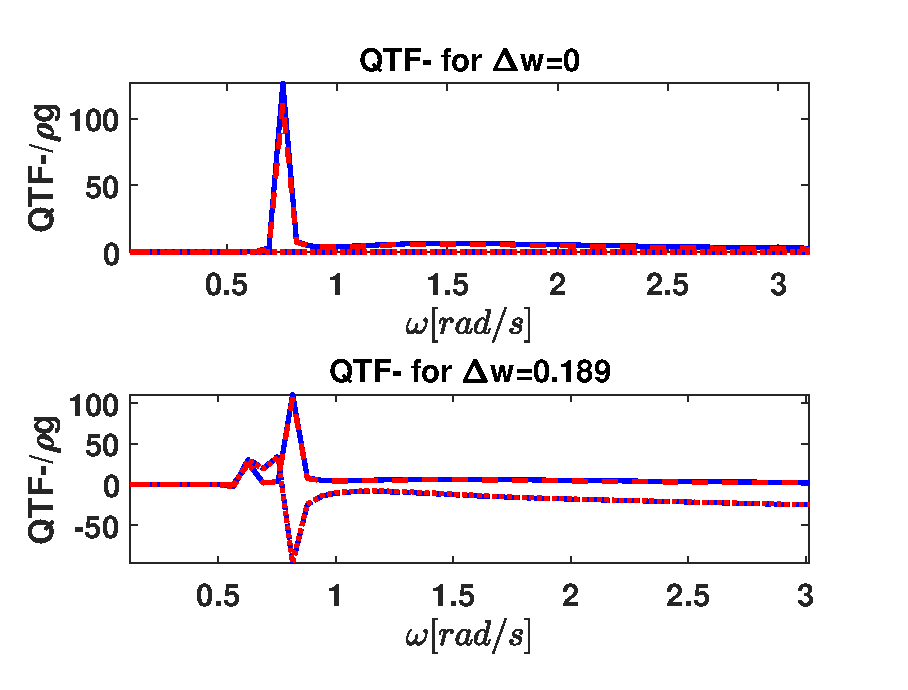
\includegraphics[scale=0.5,trim =1mm 2mm 5mm 56mm, clip]{figures/Cylinder/QTFpitch_diag.eps}	
}
	\caption{Comparison of the off-diagonal difference frequency QTF for the Cylinder (test case \textbf{8b\_QTF\_Cylinder}) between HYDROSTAR, real part (blue, solid-line), imaginary part (blue, dashed-dot line) and NEMOH, real part (red, dashed-line), imaginary part (red, dotted-line). On the top-left is for surge, on the top-right for heave (the first off-diagonal) and the bottom for pitch (the third off-diagonal)}\label{fig:QTFM_diag_Cylinder}
\end{figure}

\item \textbf{9\_QTF\_OC4\_Semisubmersible}: full body mesh with lid panels, CoG $(0,0,0)$, water depth 200 m, wave direction $0^{\circ}$ and $30^{\circ}$, bi-directional QTF, the difference-frequency QTF DUOK+HASBO. The results are shown in the density plot, Fig. \ref{fig:QTFM_OC4} and in the off-diagonal line plot, Fig. \ref{fig:QTFM_diag_OC4}, of the bi-directional QTF $(\beta_1,\beta_2)=(0^{\circ},30^{\circ})$. The mesh used was obtained using GMSH \cite{gmsh} and is shown in Fig. \ref{fig:meshesOC4}.

\begin{figure}[h!tbp]
\centering
%\subfigure{
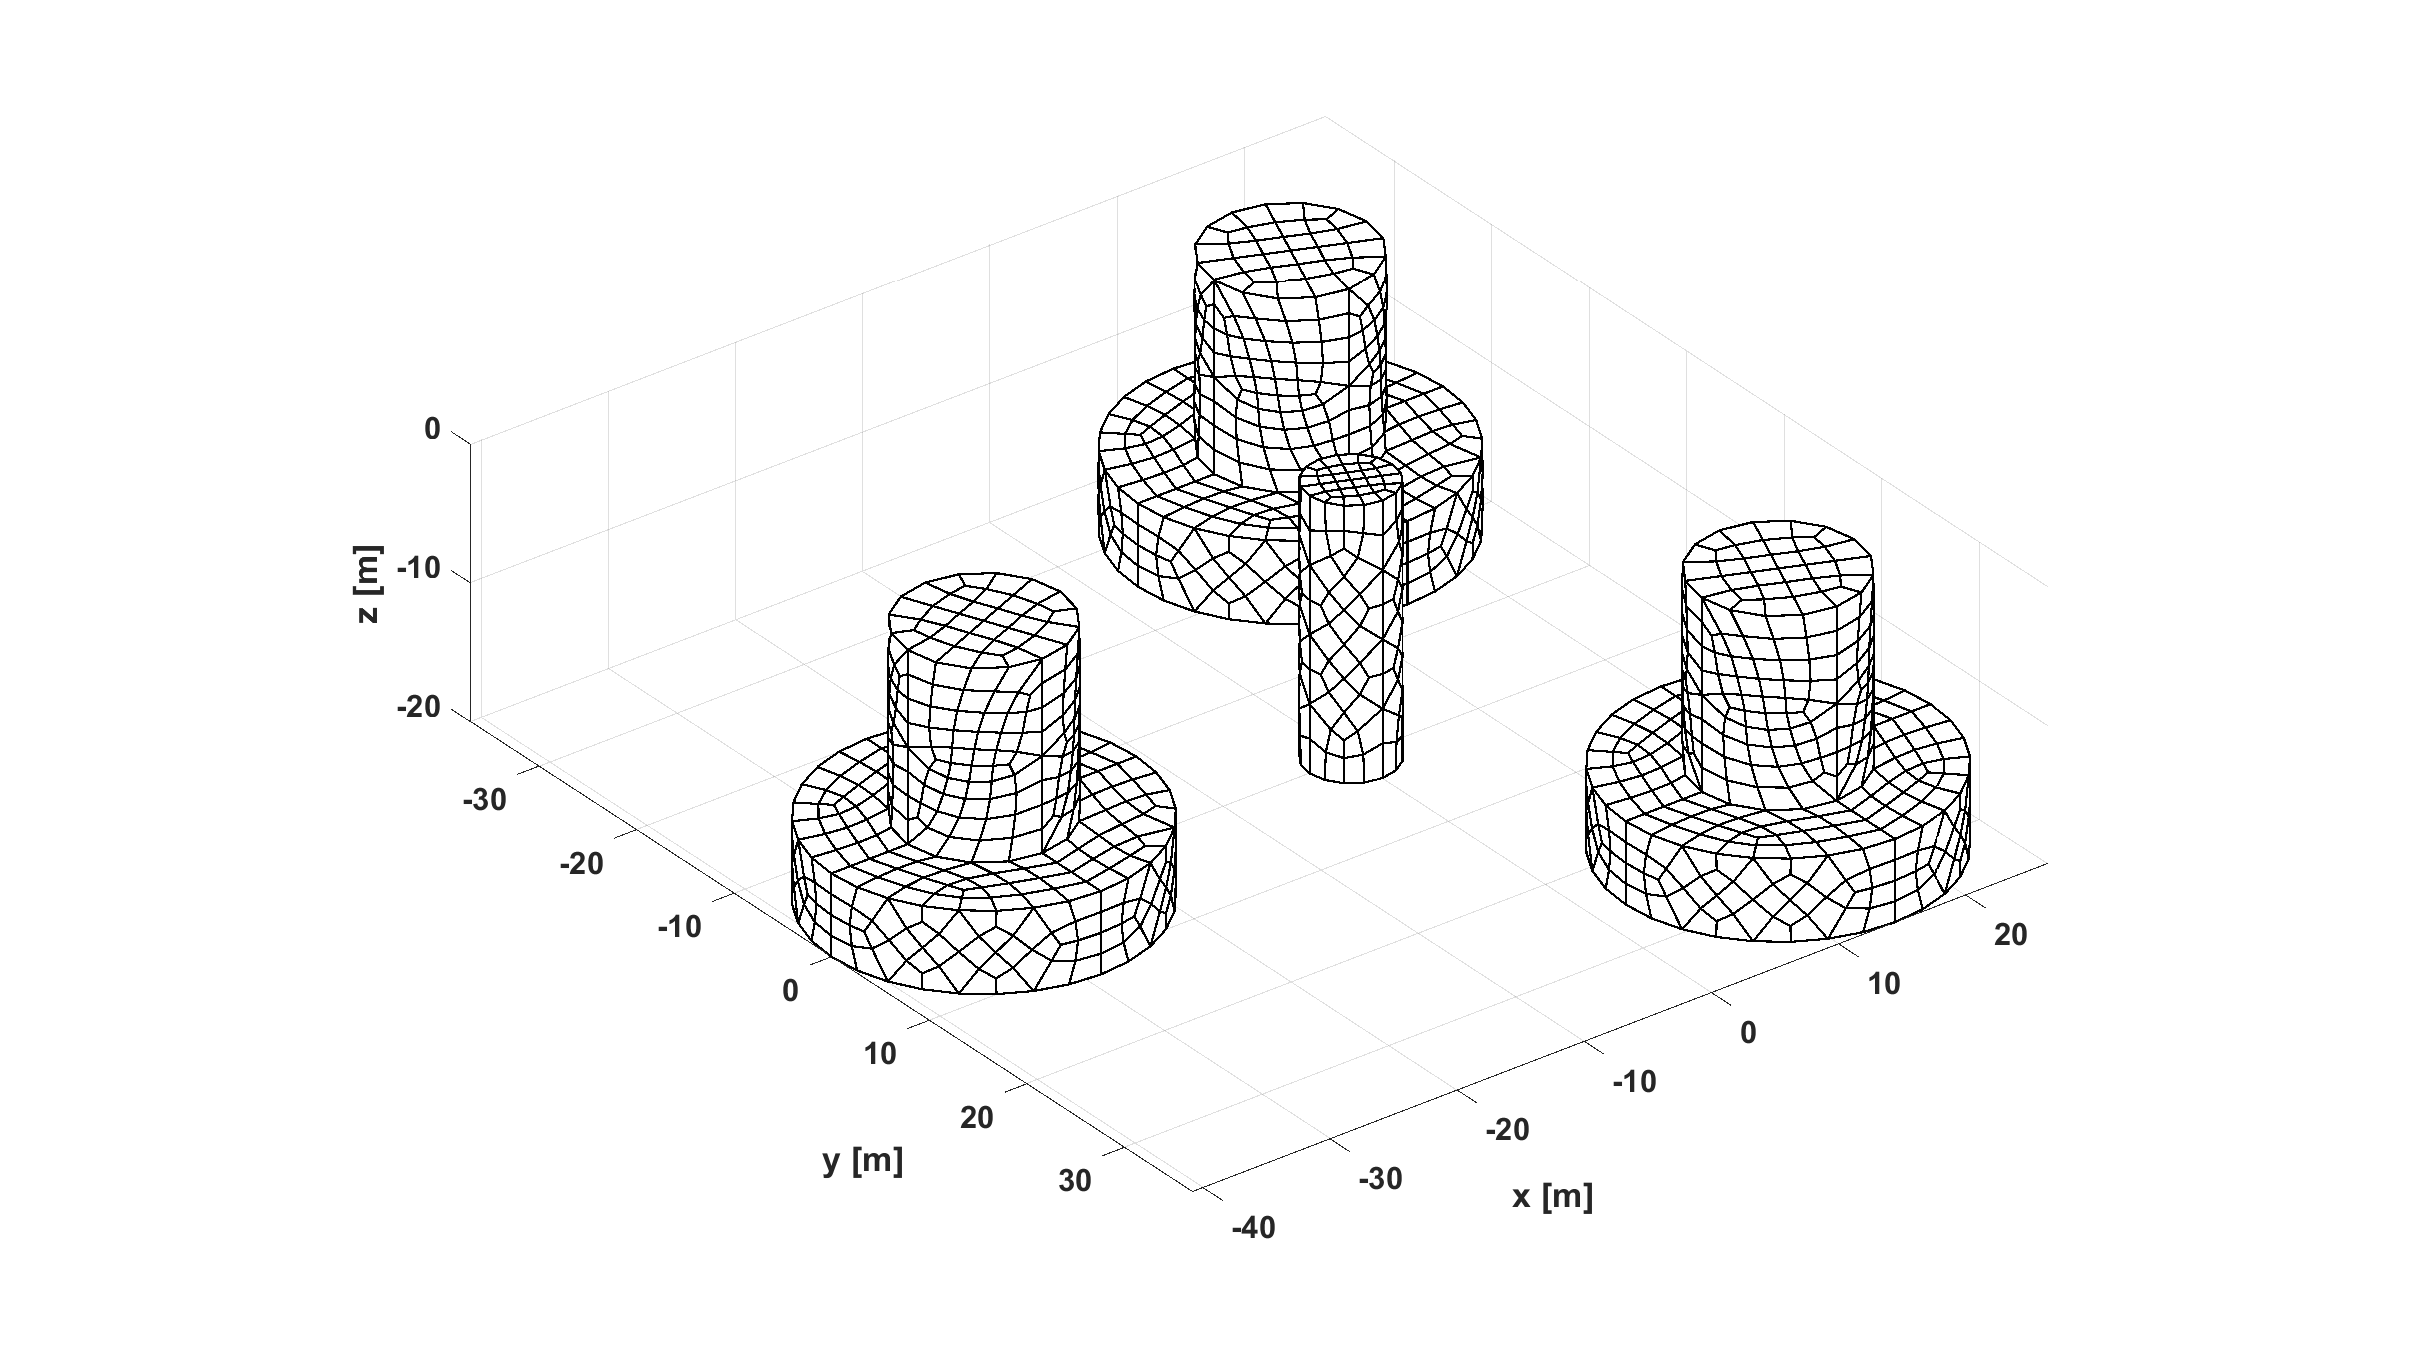
\includegraphics[scale=0.5,trim = 50mm 15mm 50mm 18mm, clip]{figures/OC4/bodymesh.eps}	
%}
\caption{Body boundary mesh for for the OC4-platform used for test case \textbf{9\_QTF\_OC4\_Semisubmersible}.}\label{fig:meshesOC4}
\end{figure}



\begin{figure}[h!tbp]
	\centering
\subfigure{
	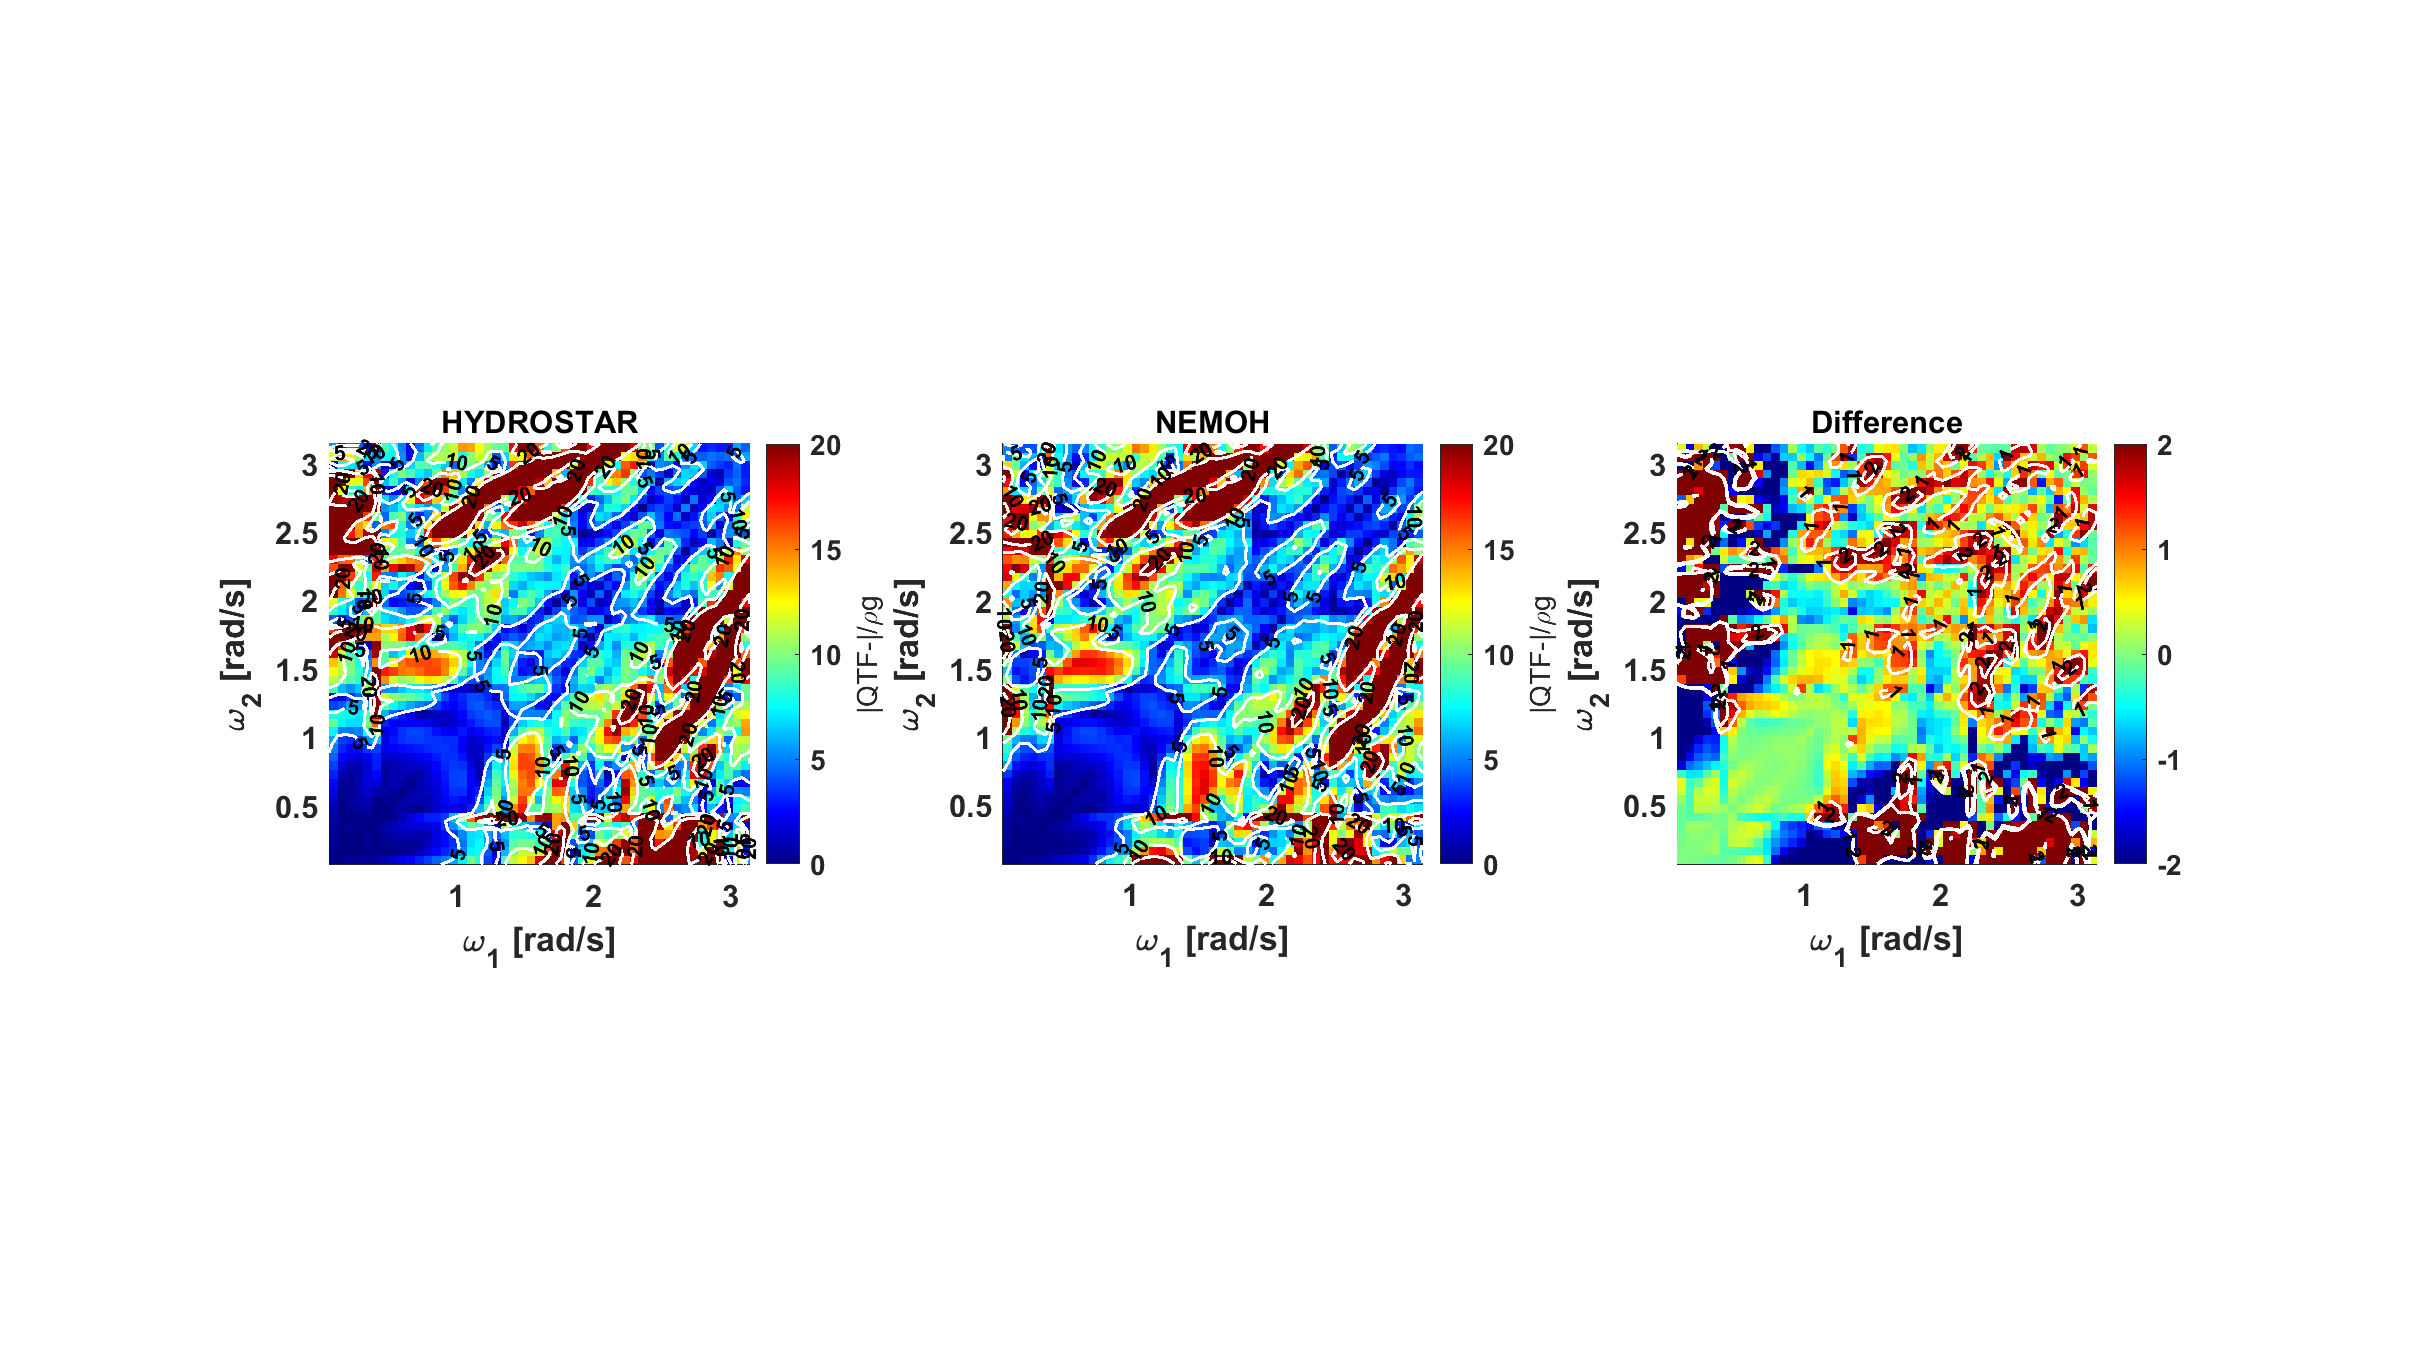
\includegraphics[scale=0.4,trim = 20mm 72mm 20mm 59mm, clip]{figures/OC4/QTFM_Surge_beta030.eps}	
}
\subfigure{
	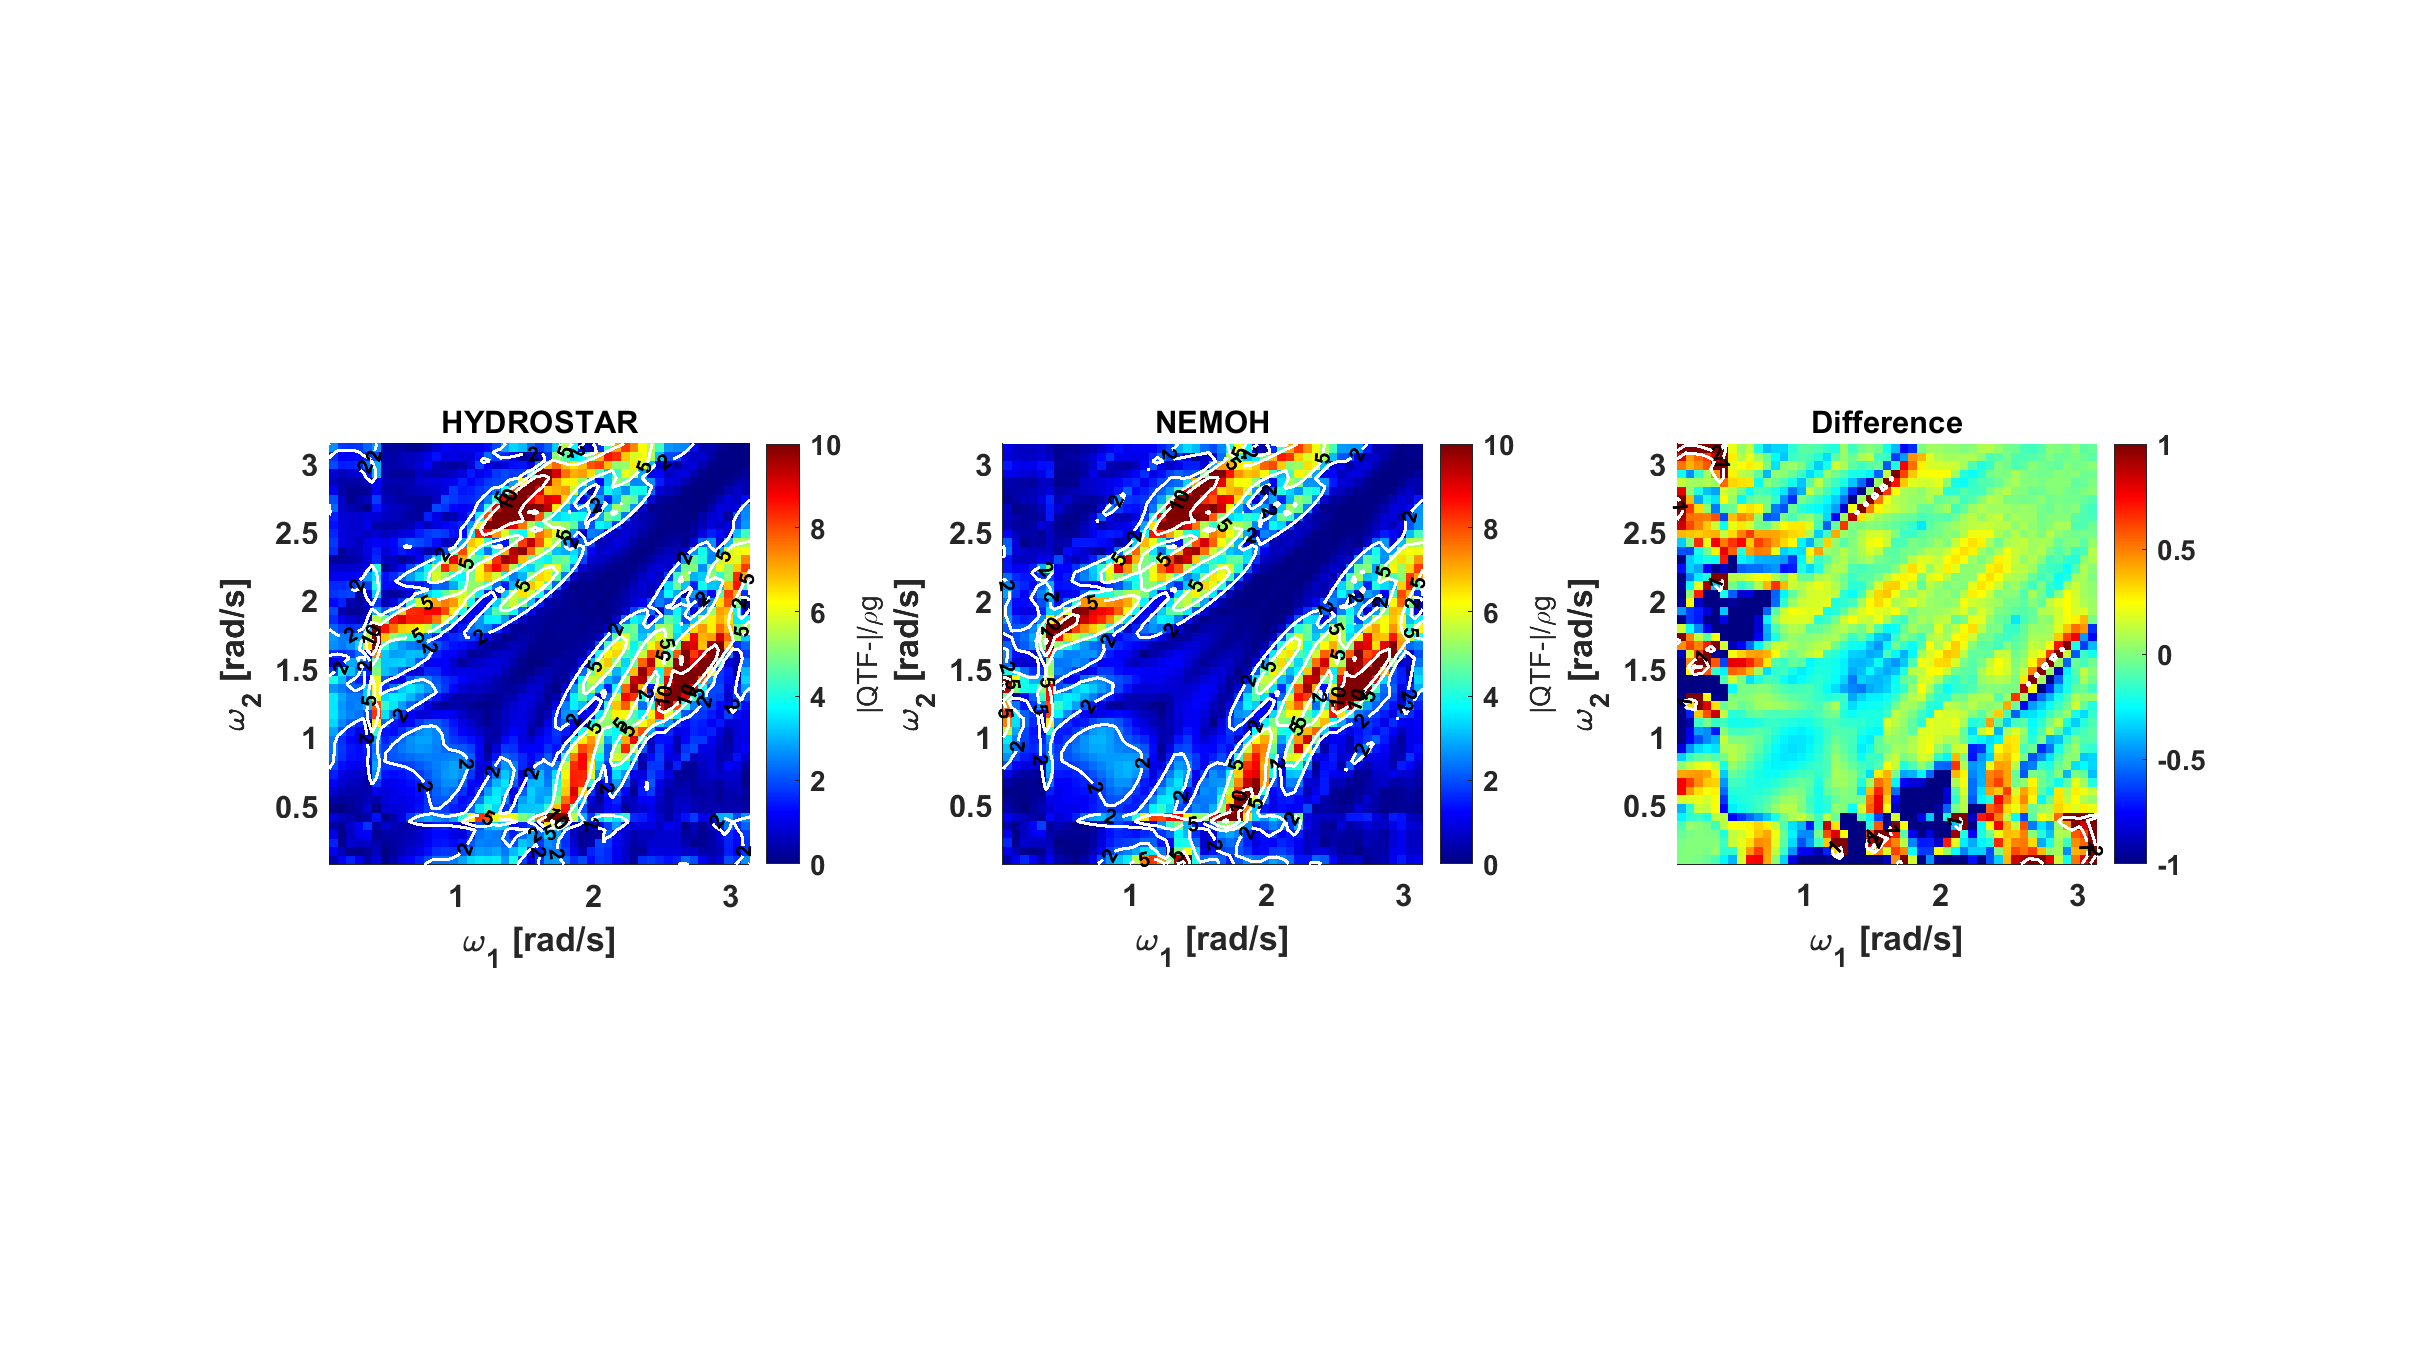
\includegraphics[scale=0.4,trim = 20mm 72mm 20mm 71mm, clip]{figures/OC4/QTFM_Heave_beta030.eps}	
}
\subfigure{
	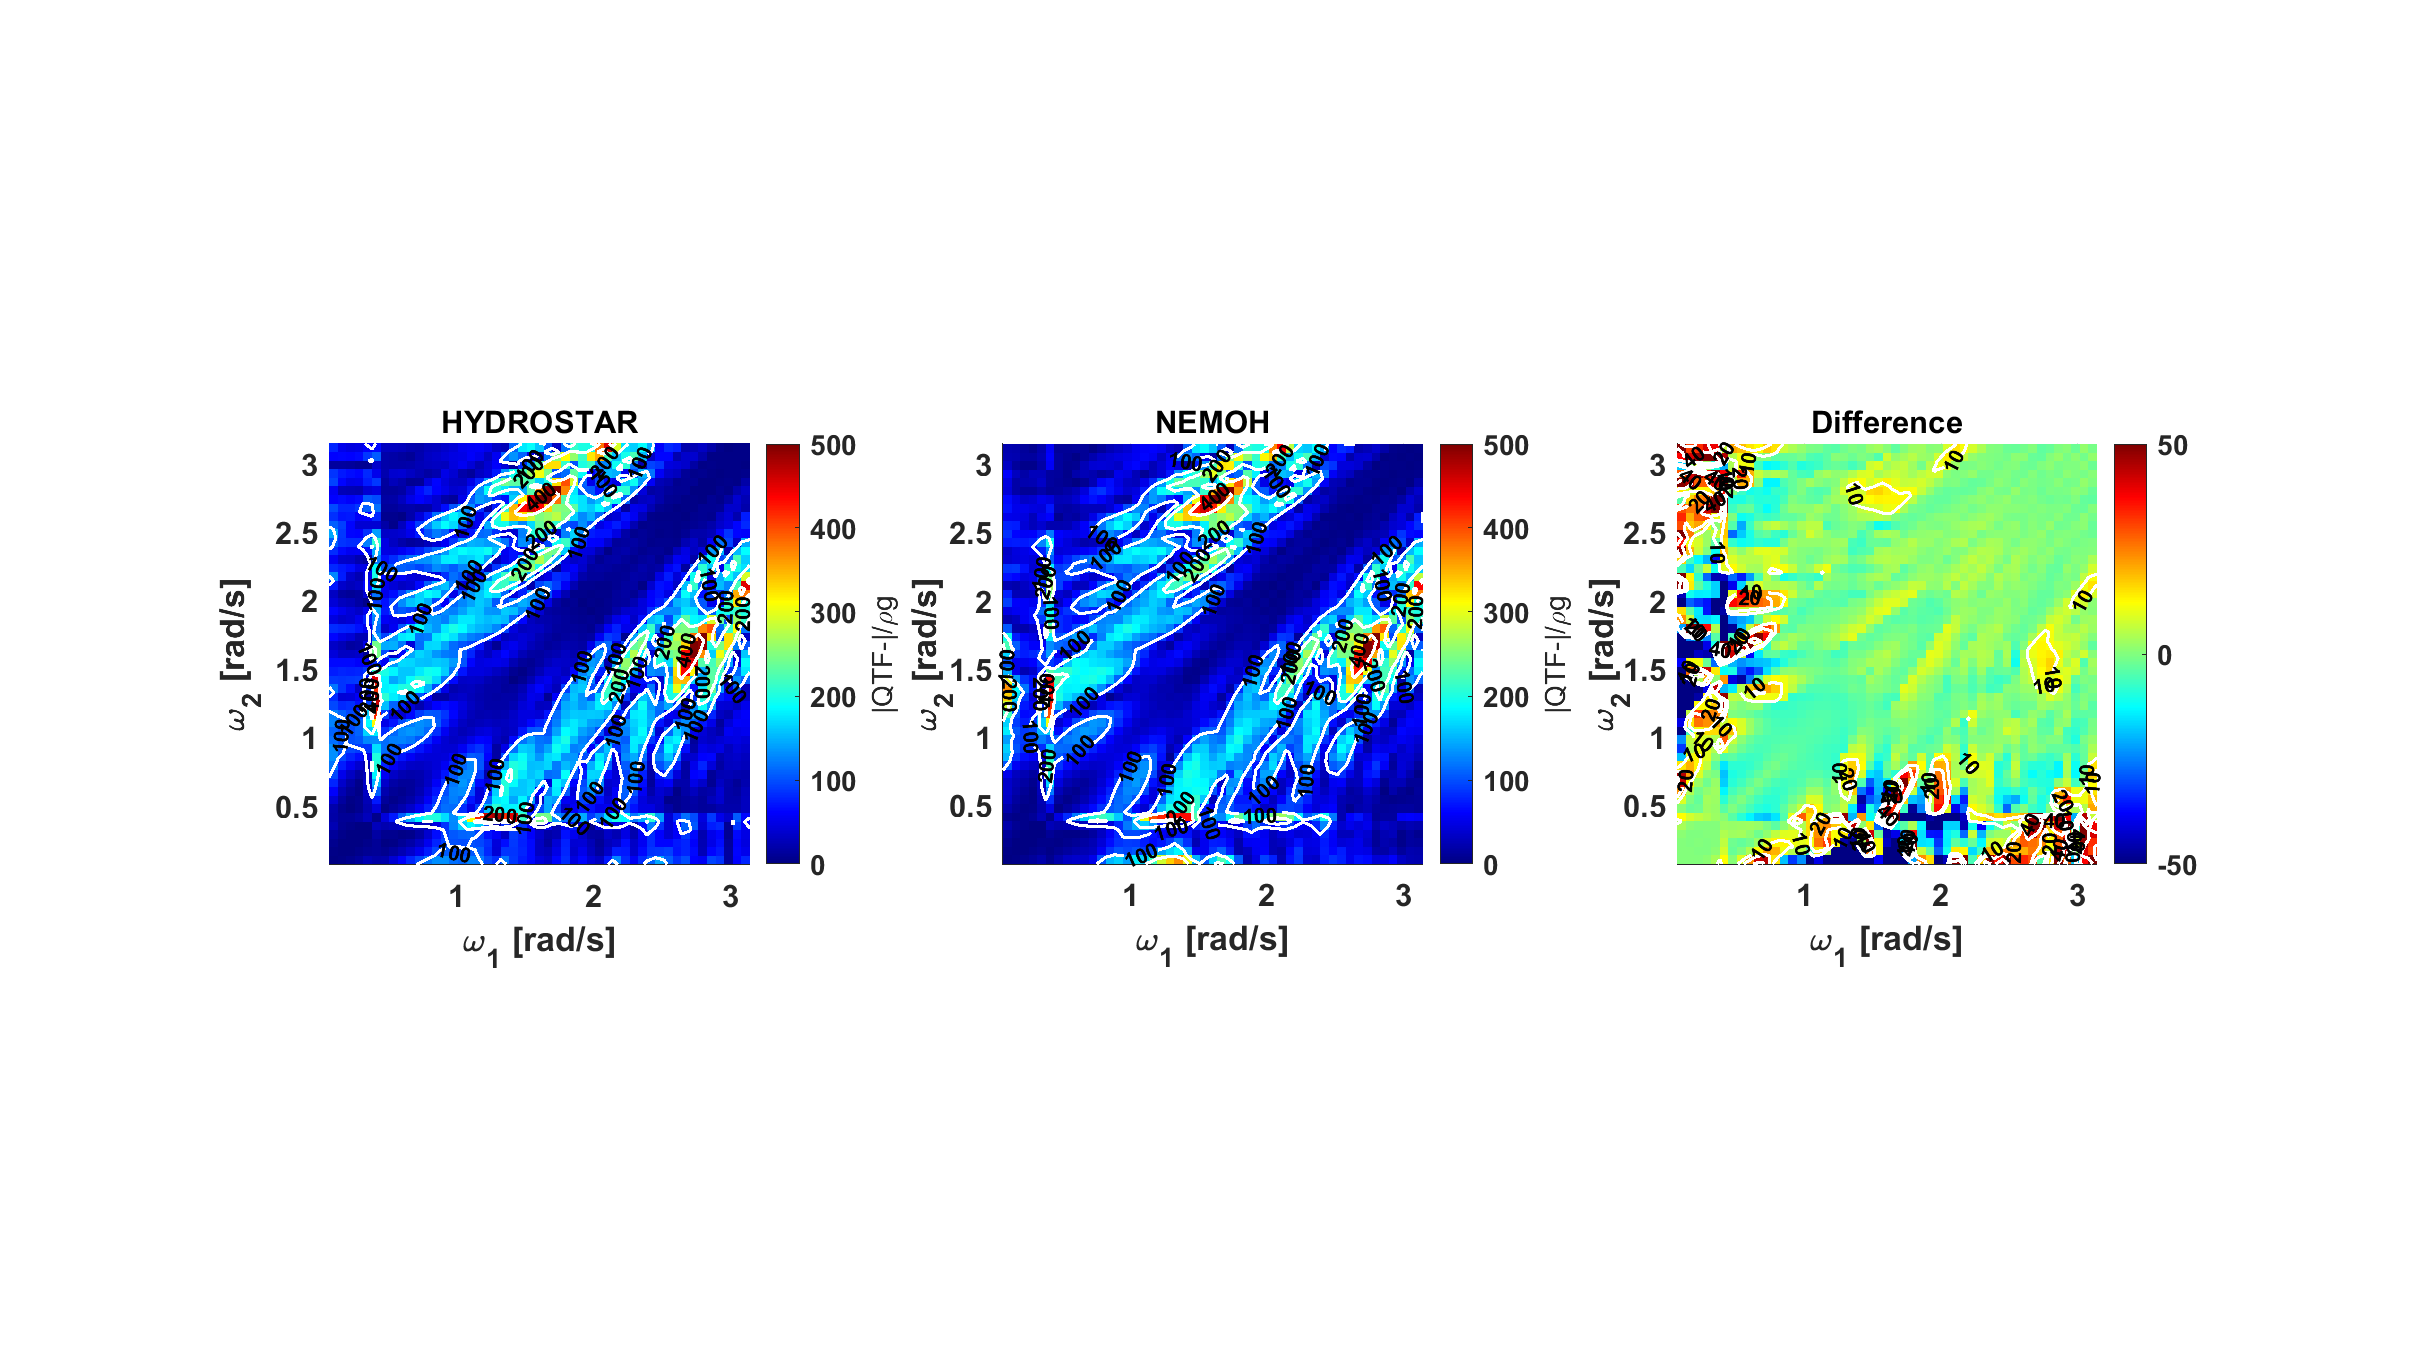
\includegraphics[scale=0.4,trim = 20mm 62mm 20mm 71mm, clip]{figures/OC4/QTFM_Pitch_beta030.eps}	
}
	\caption{Density plots of the normalized bi-directional, $(\beta_1,\beta_2)=(0^{\circ},30^{\circ})$, surge difference frequency QTF magnitude (without the free-surface integrals) for the floating OC4-semisubmersible platform (test case \textbf{9\_QTF\_OC4\_Semisubmersible}); on the top, middle and bottom rows are for surge, heave and pitch, respectively. HYDROSTAR results are on the left column, NEMOH results are on the middle column and the difference on the right column.}\label{fig:QTFM_OC4}
\end{figure}

\begin{figure}[h!tbp]
	\centering
\subfigure{
	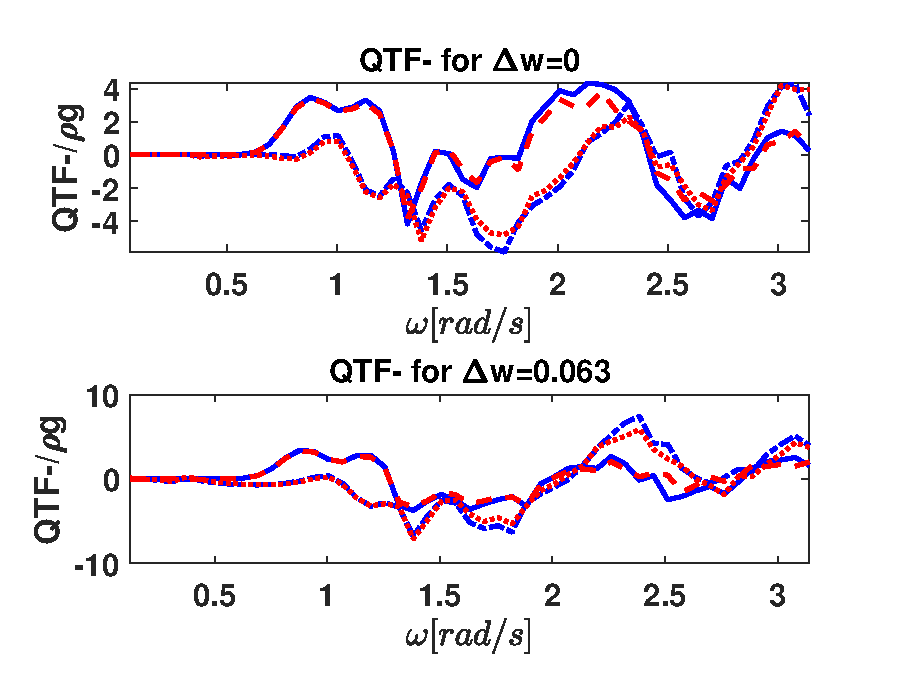
\includegraphics[scale=0.5,trim = 3mm 10mm 5mm 56mm, clip]{figures/OC4/QTFM_Surge_beta030_diag.eps}	
}
\subfigure{
	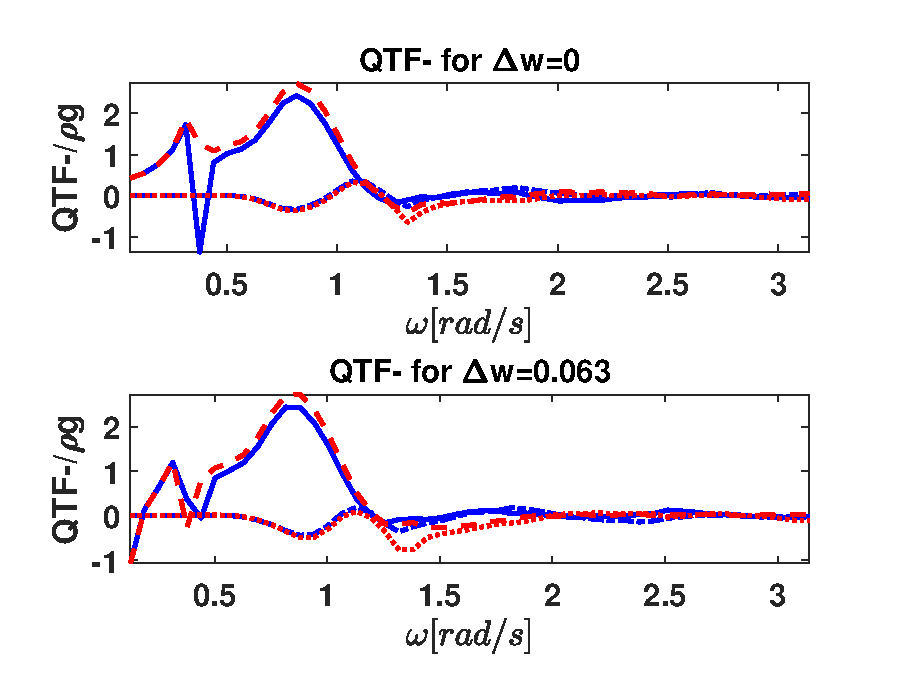
\includegraphics[scale=0.5,trim = 5mm 10mm 5mm 56mm, clip]{figures/OC4/QTFM_Heave_beta030_diag.eps}	
}
\subfigure{
	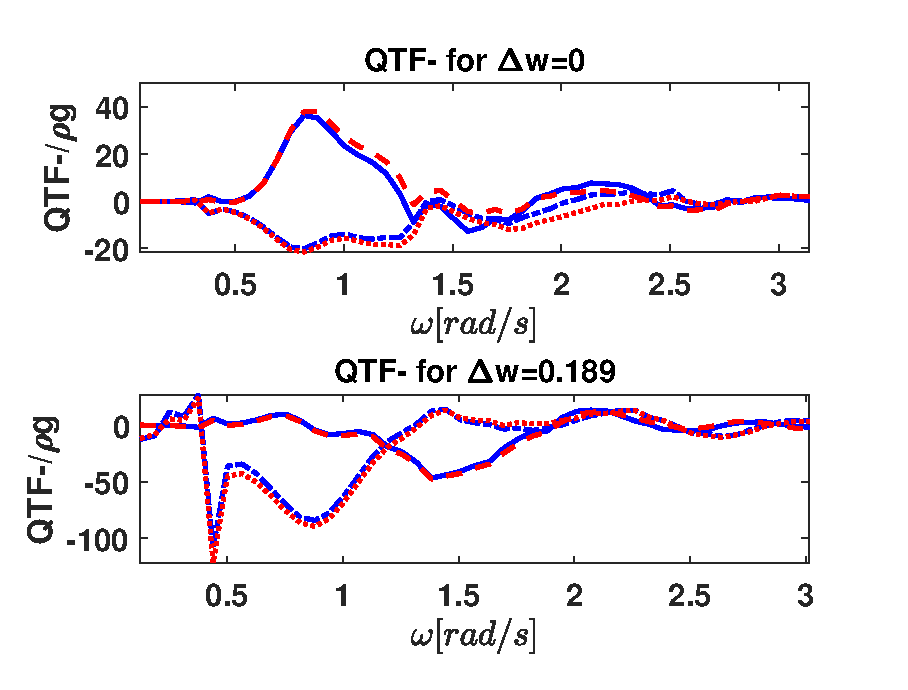
\includegraphics[scale=0.5,trim =1mm 2mm 5mm 56mm, clip]{figures/OC4/QTFM_Pitch_beta030_diag.eps}	
}
	\caption{Comparison of the off-diagonal bi-directional, $(\beta_1,\beta_2)=(0^{\circ},30^{\circ})$, difference frequency QTF for the OC4-semisubmersible platform (test case \textbf{9\_QTF\_OC4\_Semisubmersible})between HYDROSTAR, real part (blue, solid-line), imaginary part (blue, dashed-dot line) and NEMOH, real part (red, dashed-line), imaginary part (red, dotted-line). On the top-left is for surge, on the top-right for heave (the first off-diagonal) and the bottom for pitch (the third off-diagonal)}\label{fig:QTFM_diag_OC4}
\end{figure}

\item \textbf{10a\_QTF\_SOFTWIND}: half symmetric body mesh with lid panels, CoG $(0,0,-71.56)$, water depth 200 m, wave direction $0^{\circ}$ and $30^{\circ}$, bi-directional QTF, the difference-frequency QTF DUOK+HASBO. The results are shown in the density plot, Fig. \ref{fig:QTFM_SOFTWIND} and in the off-diagonal line plot, Fig. \ref{fig:QTFM_diag_softwind}, of the bi-directional QTF $(\beta_1,\beta_2)=(0^{\circ},30^{\circ})$. The mesh used was obtained using GMSH \cite{gmsh} and is shown in Fig. \ref{fig:meshesSoftwind}.

\begin{figure}[h!tbp]
\centering
\subfigure{
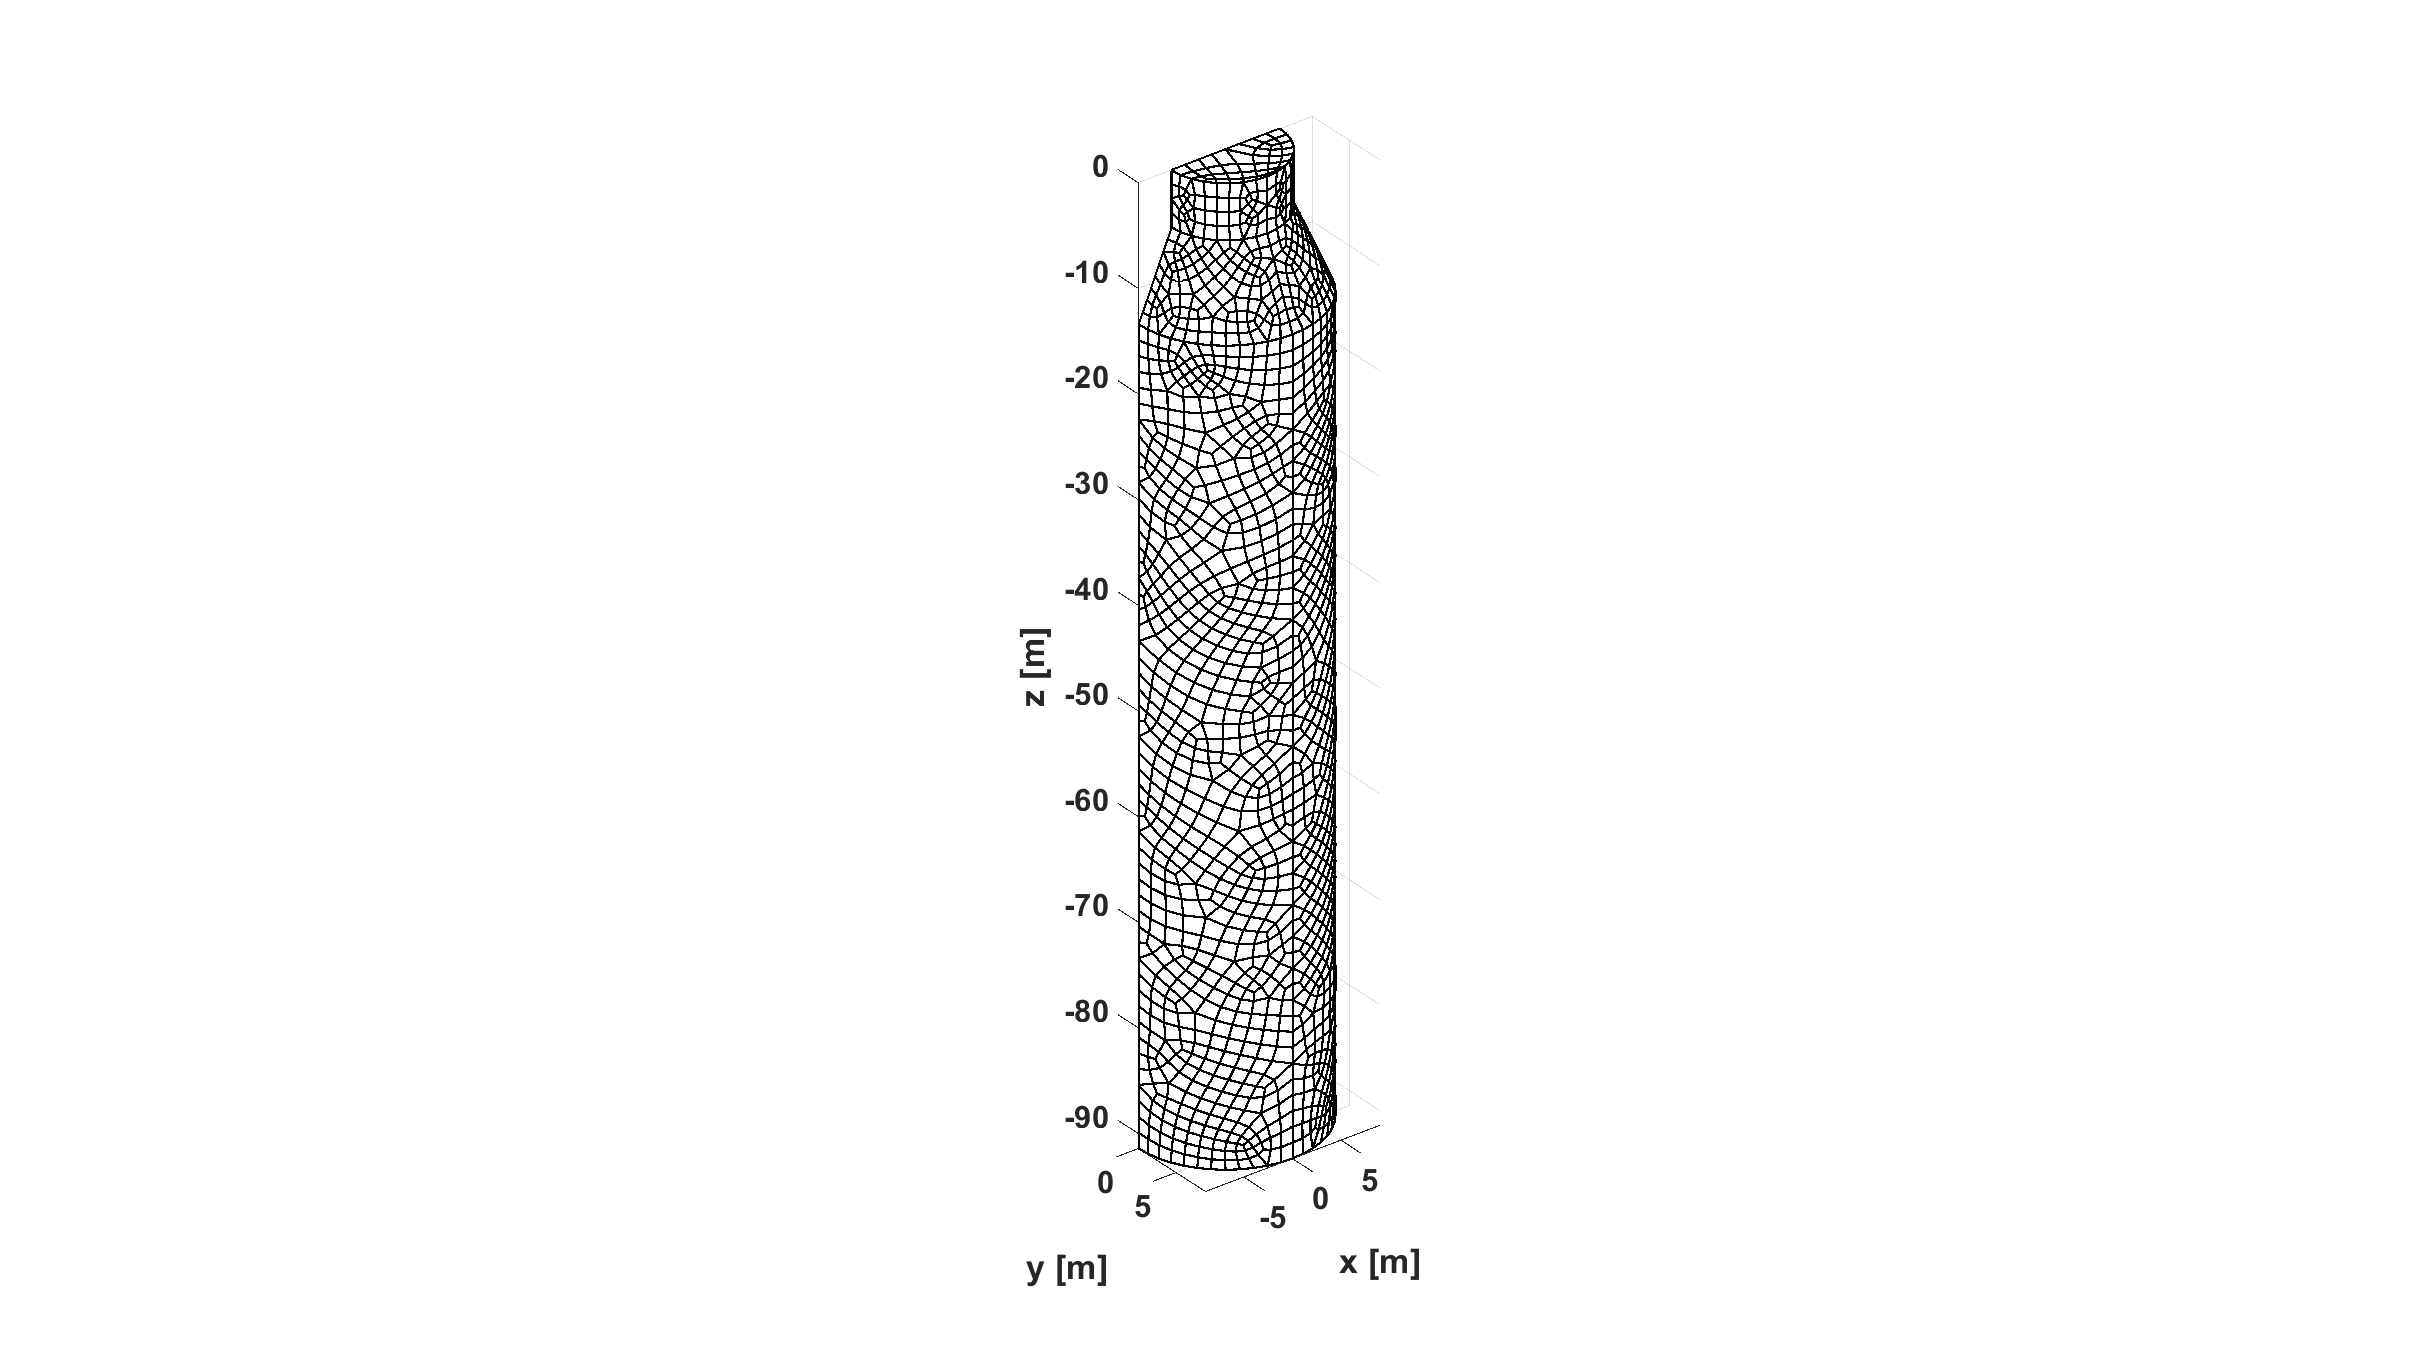
\includegraphics[scale=0.45,trim = 160mm 8mm 180mm 18mm, clip]{figures/Softwind/bodymesh.eps}	
}
\subfigure{
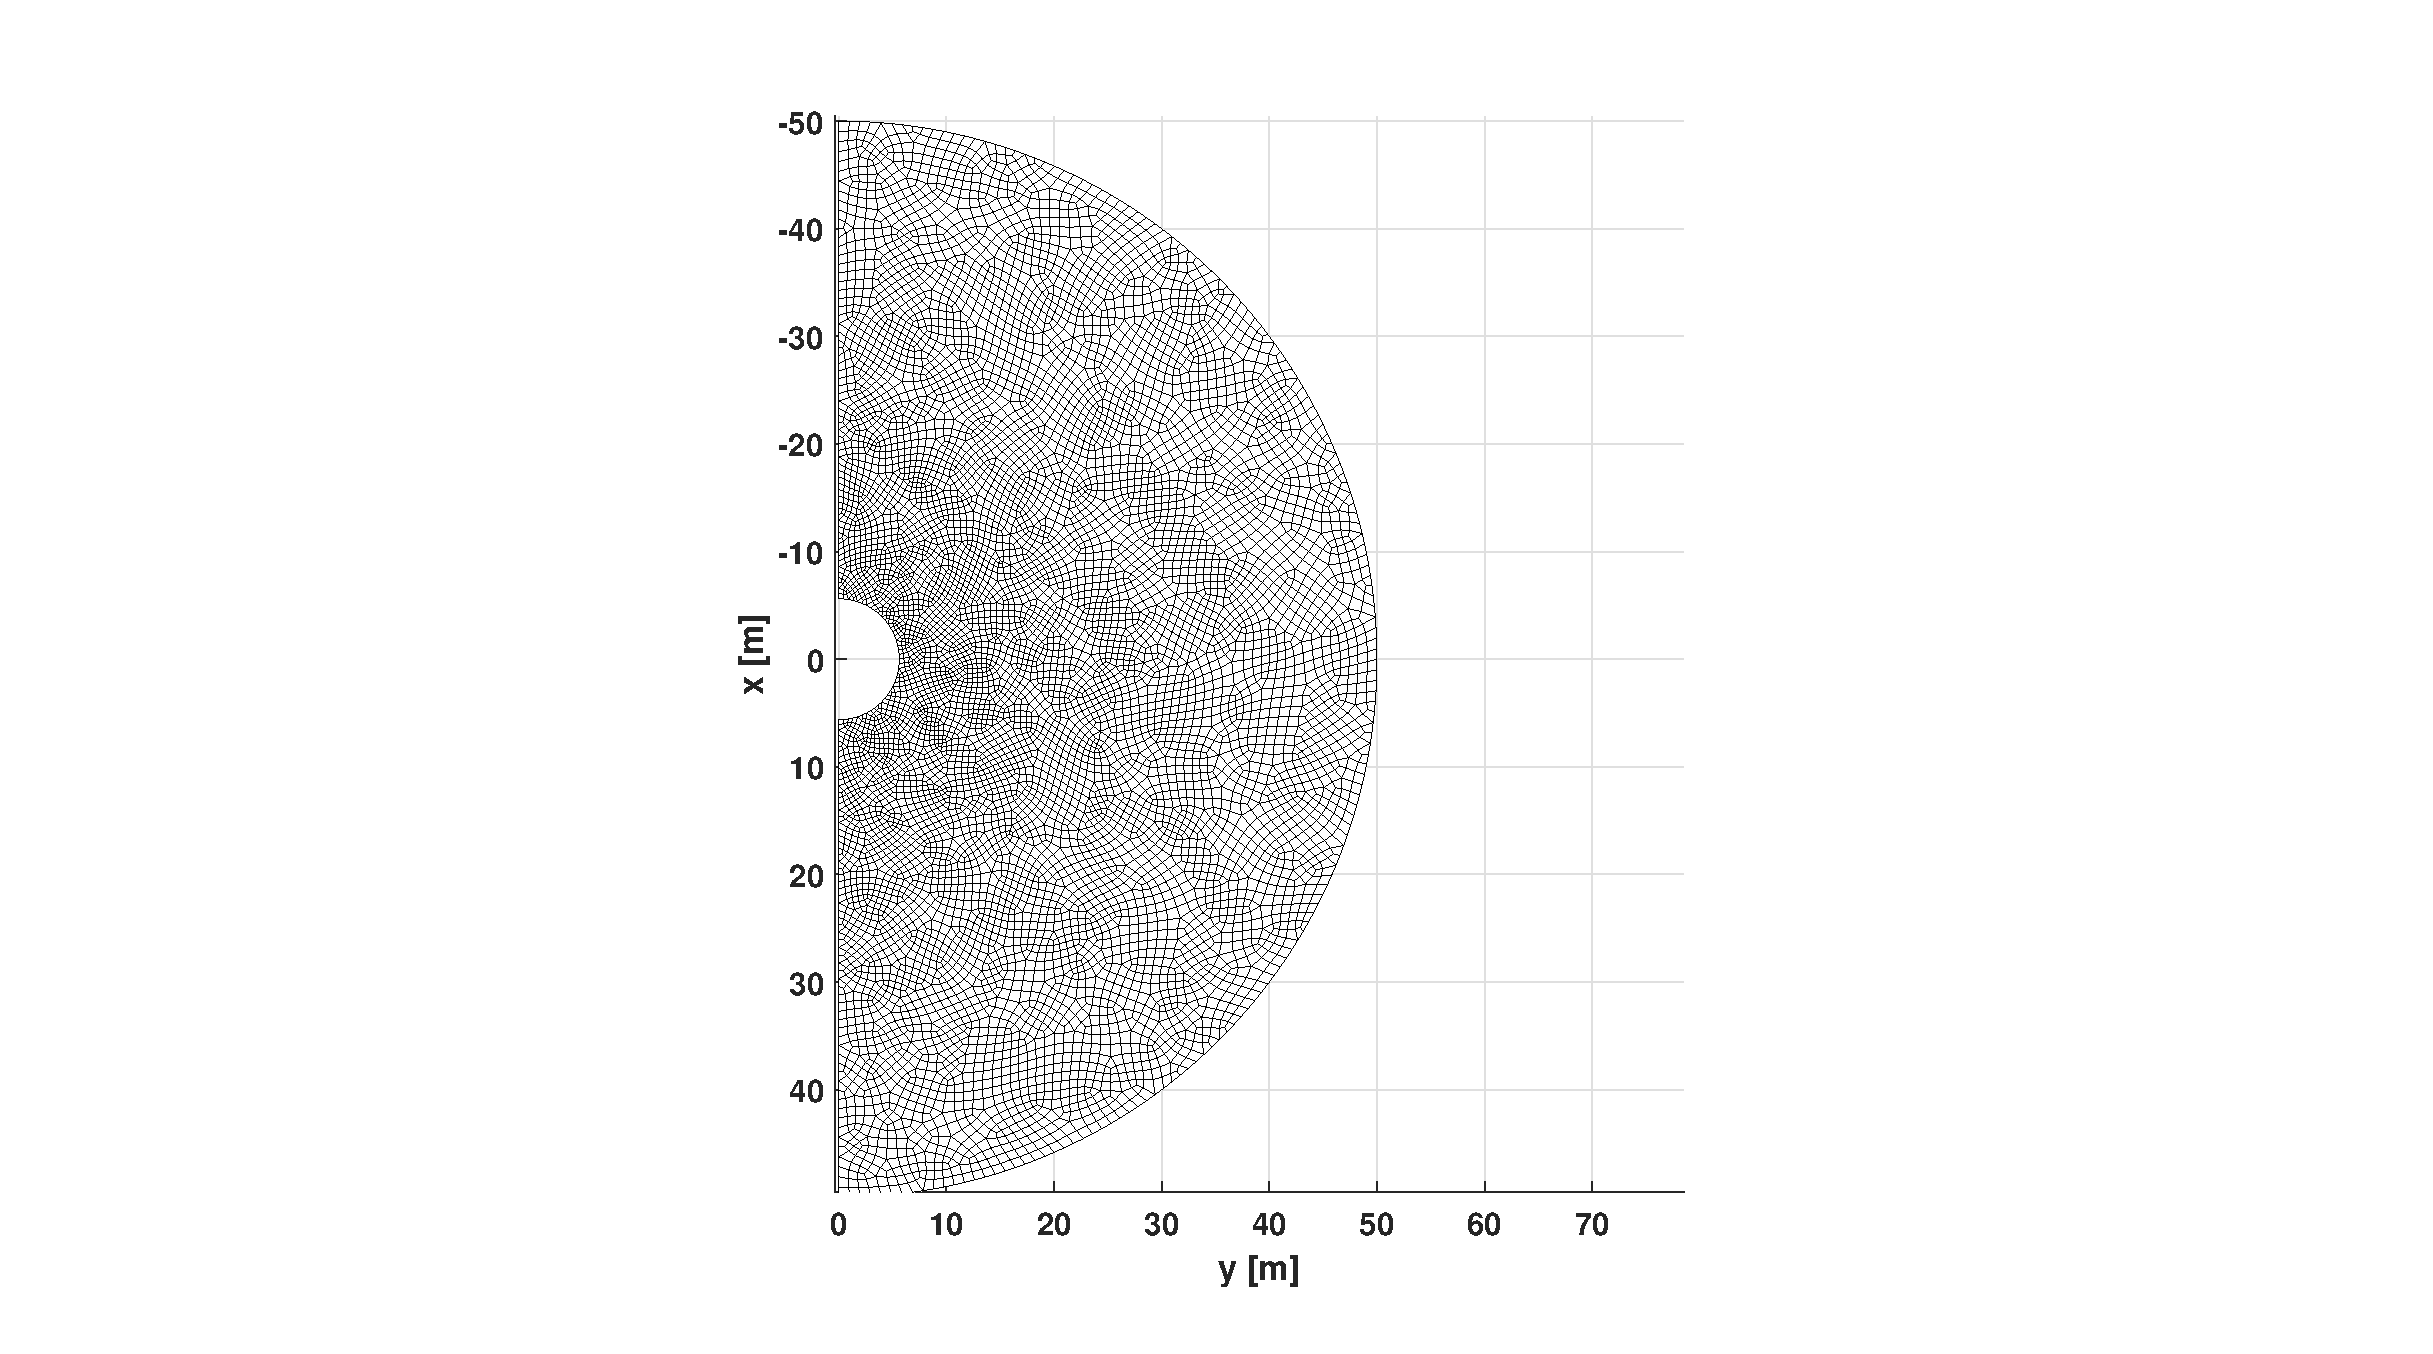
\includegraphics[scale=0.45,trim = 120mm 8mm 170mm 16mm, clip]{figures/Softwind/FSmesh.eps}	
}
\caption{Body boundary mesh and free surface mesh for the SOFTWIND platform, used in test cases \textbf{10a\_QTF\_SOFTWIND} and  \textbf{10b\_QTF\_SOFTWIND\_FS}}\label{fig:meshesSoftwind}
\end{figure}



\begin{figure}[h!tbp]
	\centering
\subfigure{
	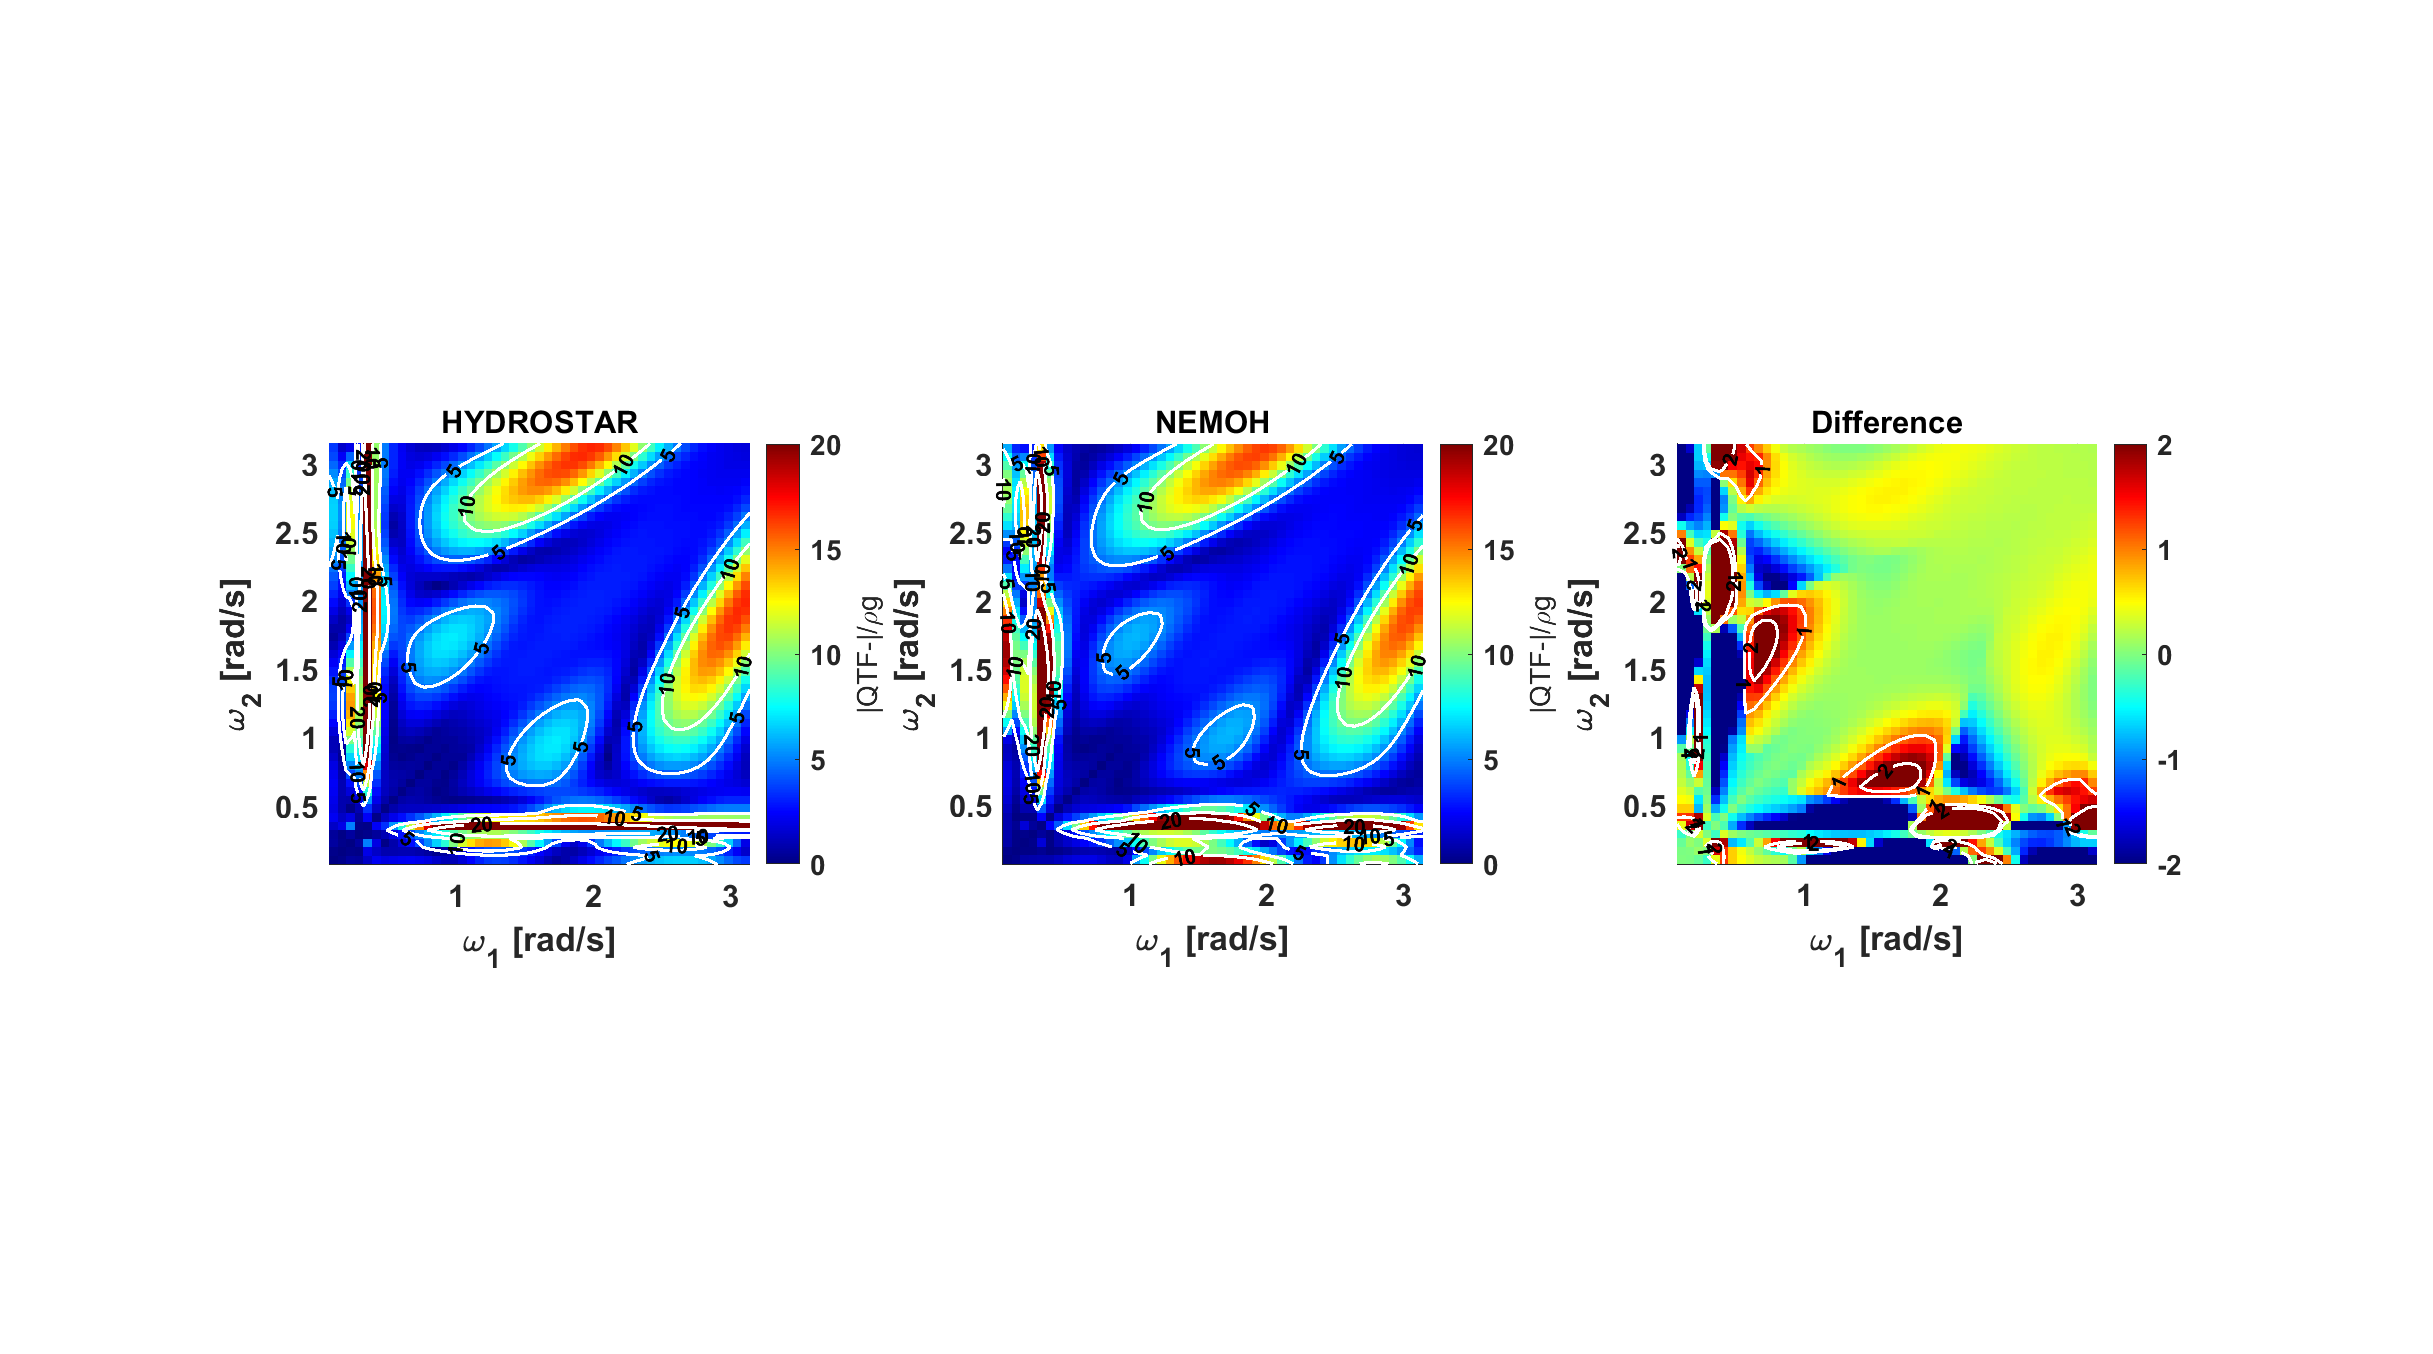
\includegraphics[scale=0.4,trim = 20mm 72mm 25mm 59mm, clip]{figures/Softwind/QTFM_Surge_beta030.eps}	
}
\subfigure{
	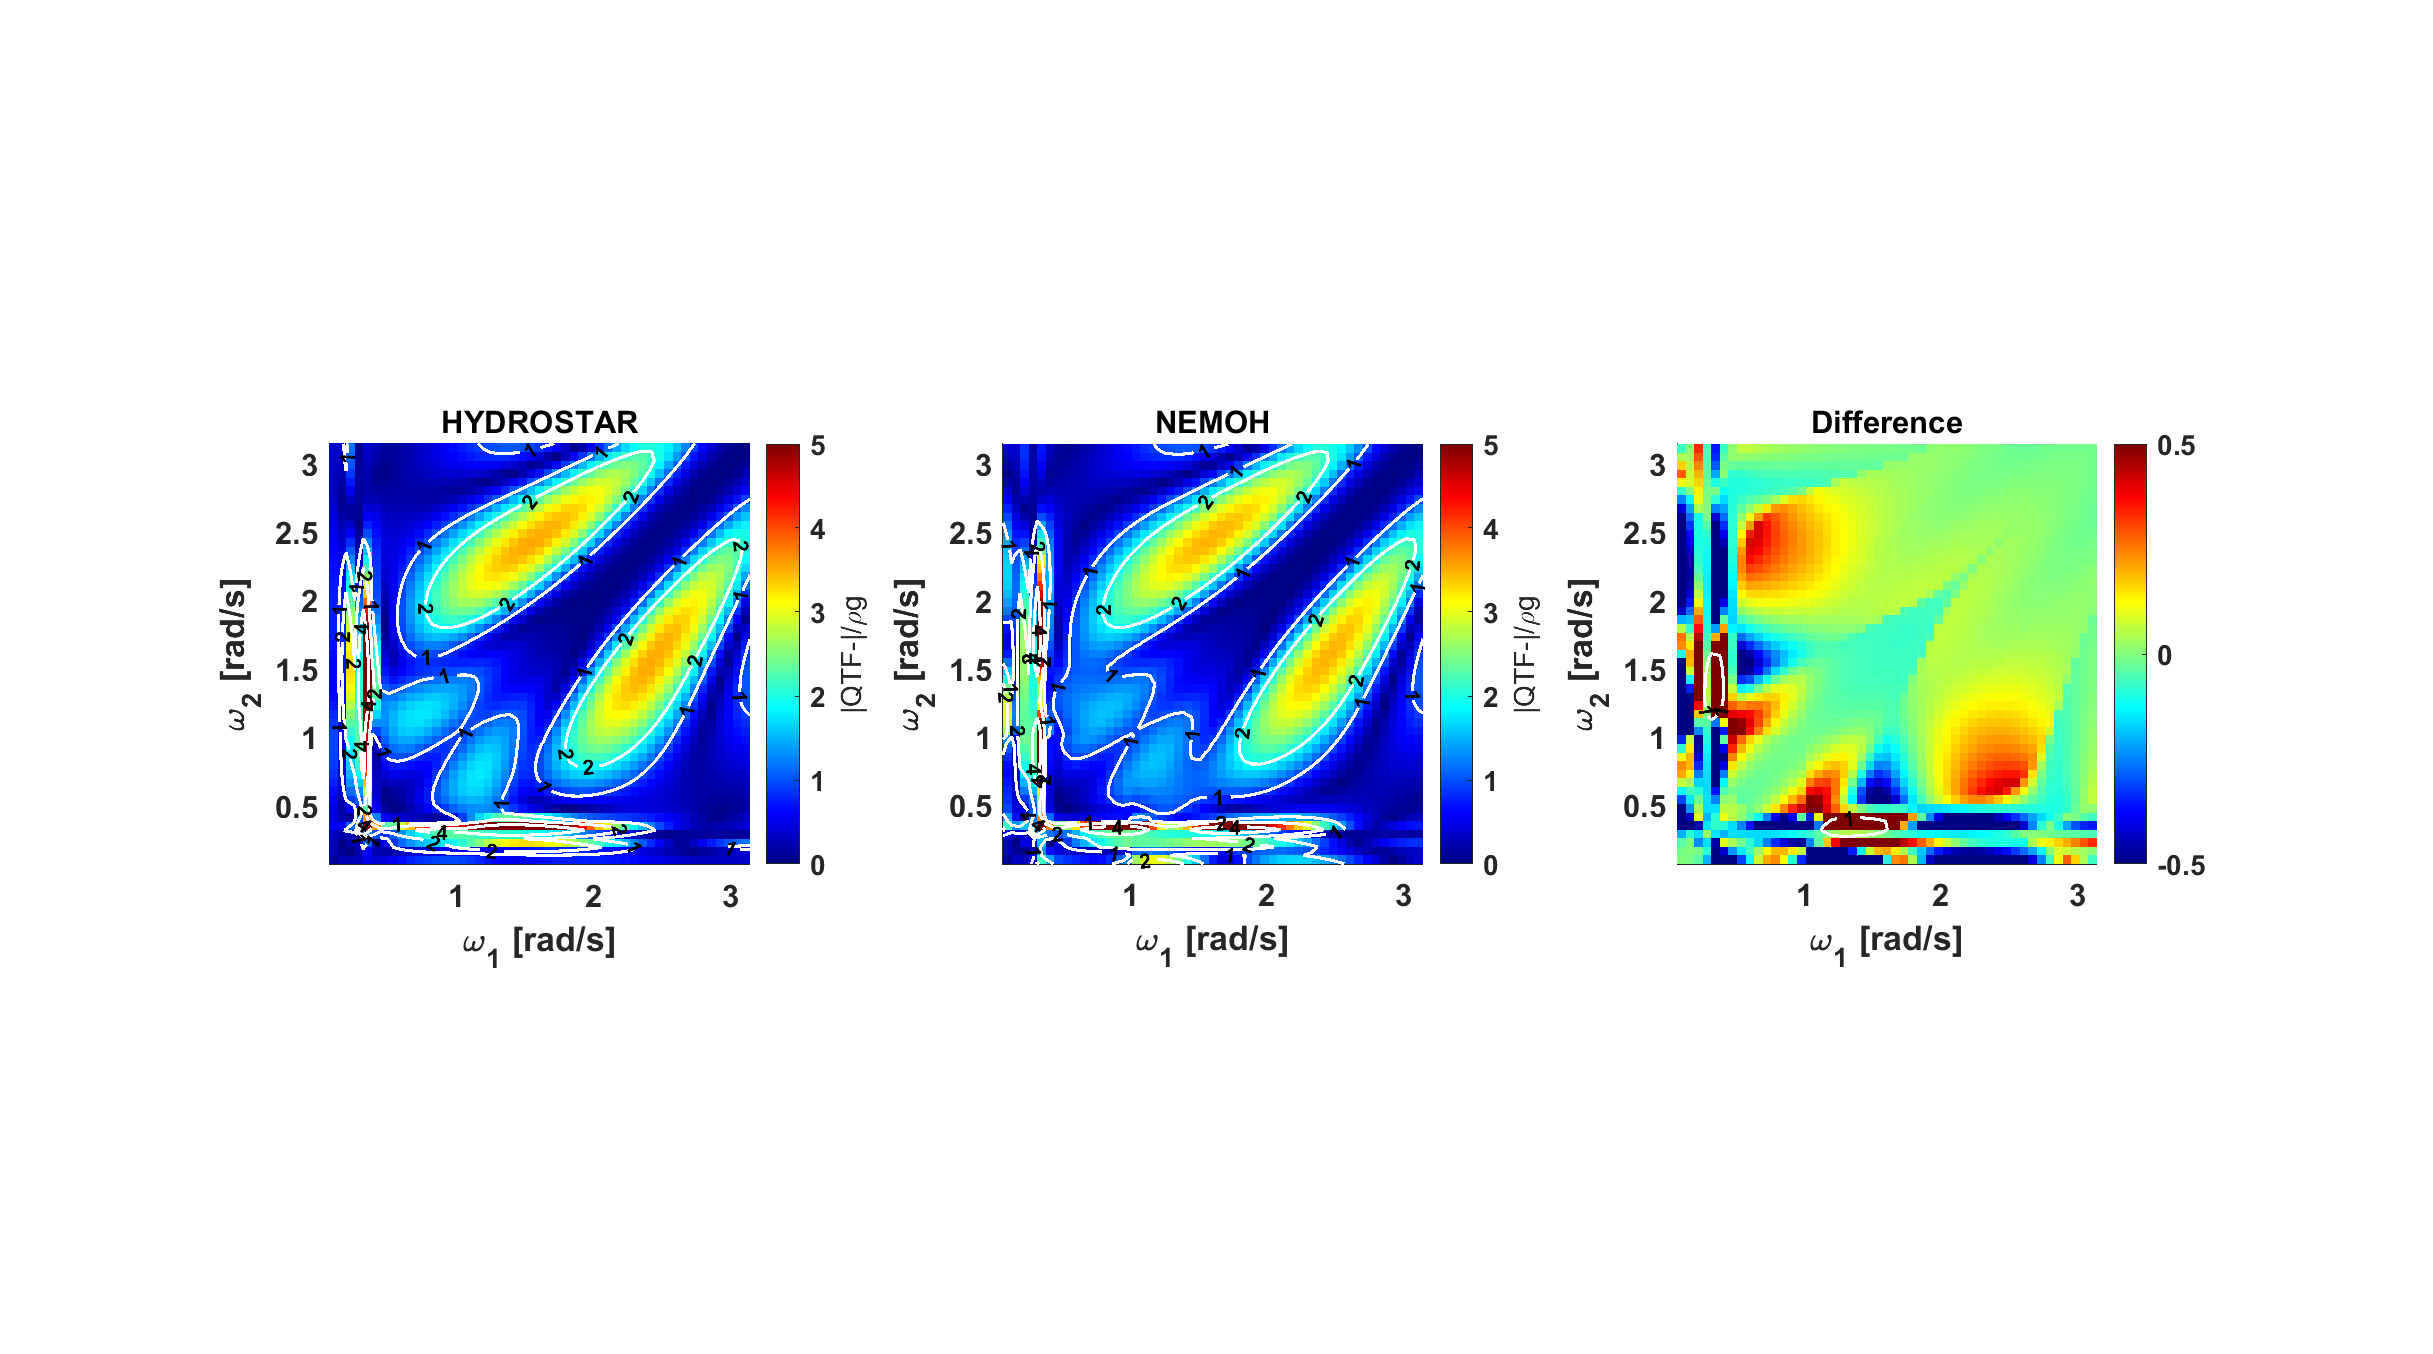
\includegraphics[scale=0.4,trim = 20mm 72mm 20mm 71mm, clip]{figures/Softwind/QTFM_Heave_beta030.eps}	
}
\subfigure{
	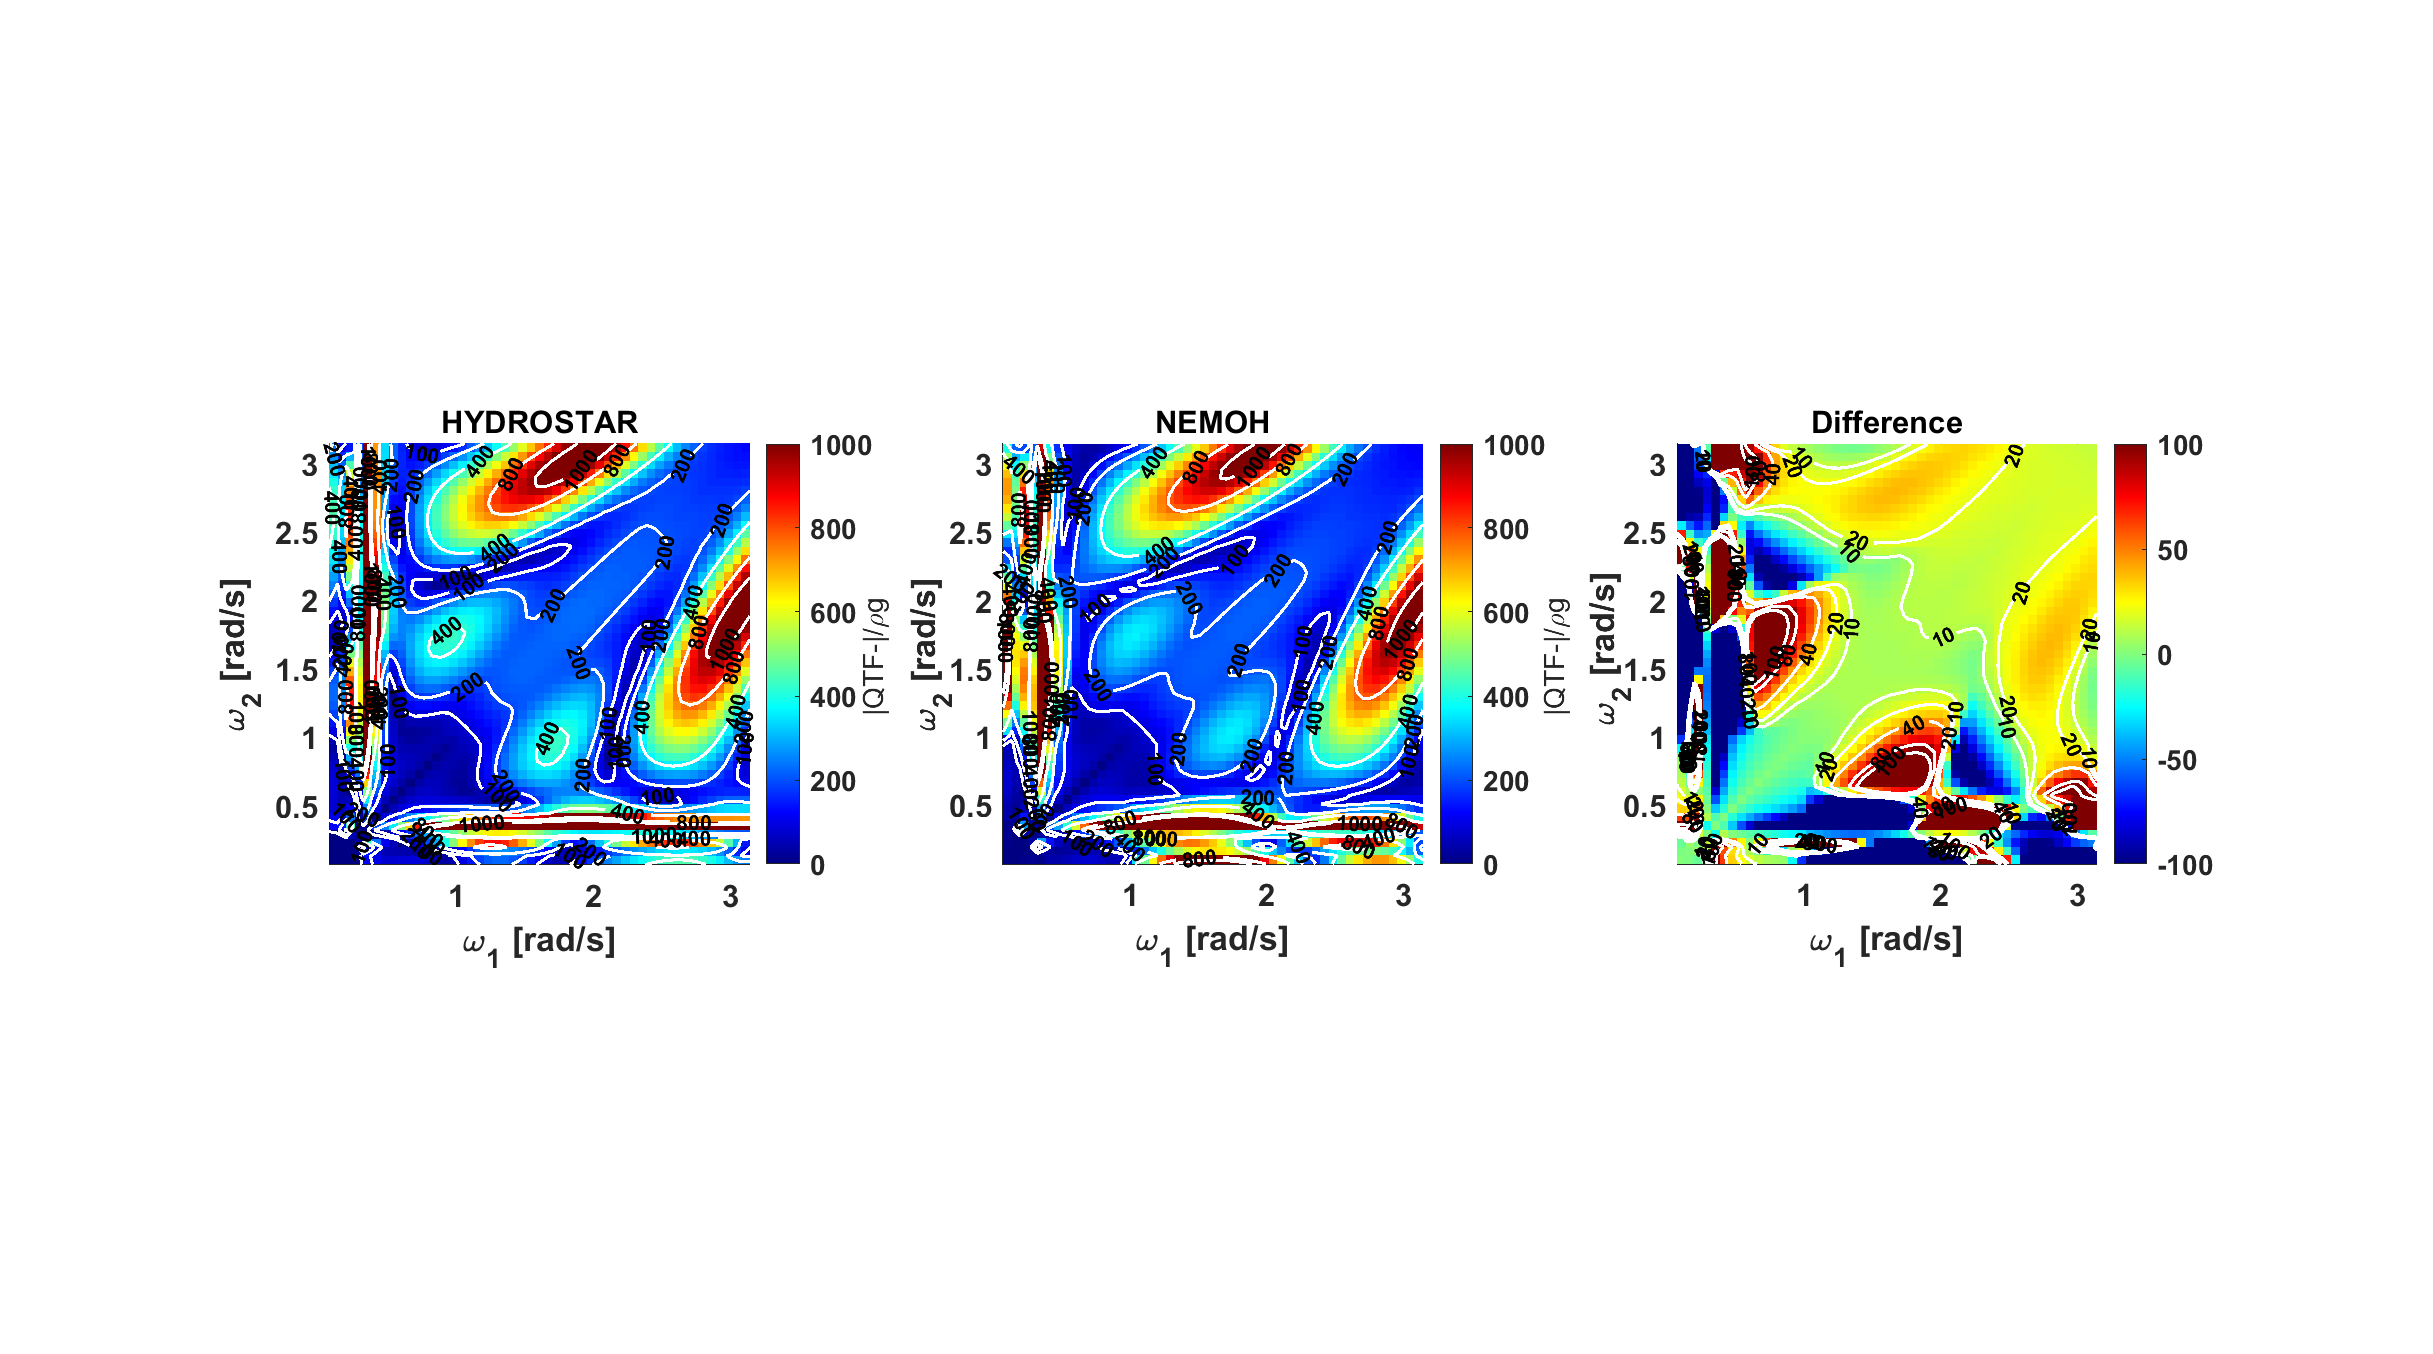
\includegraphics[scale=0.4,trim = 20mm 62mm 20mm 71mm, clip]{figures/Softwind/QTFM_Pitch_beta030.eps}	
}
	\caption{Density plots of the normalized bi-directional, $(\beta_1,\beta_2)=(0^{\circ},30^{\circ})$, surge difference frequency QTF magnitude (without the free-surface integrals) for the floating SOFTWIND platform (test case \textbf{10a\_QTF\_SOFTWIND}); on the top, middle and bottom rows are for surge, heave and pitch, respectively. HYDROSTAR results are on the left column, NEMOH results are on the middle column and the difference on the right column.}\label{fig:QTFM_SOFTWIND}
\end{figure}

\begin{figure}[h!tbp]
	\centering
\subfigure{
	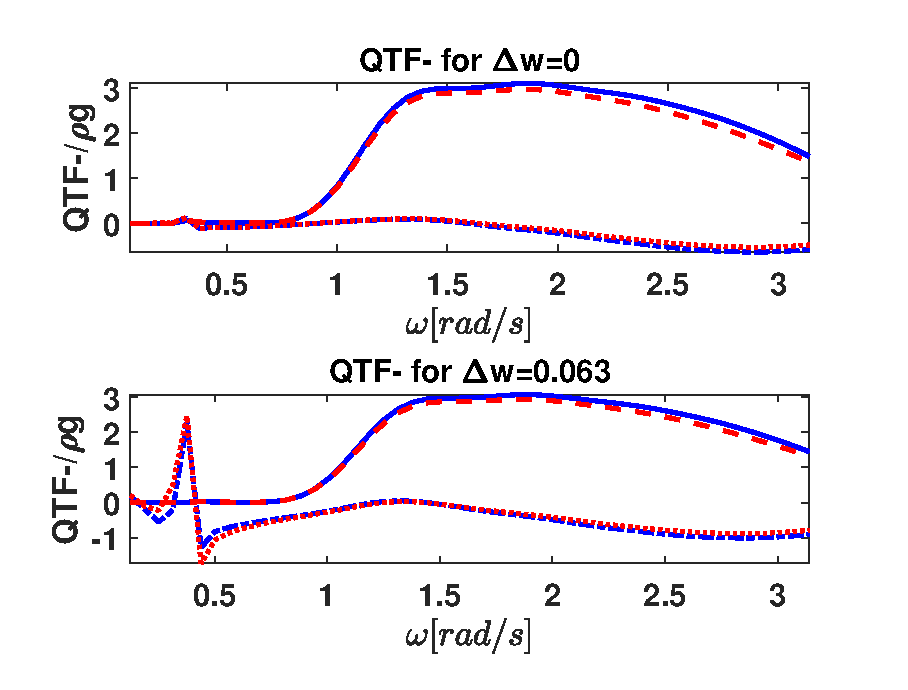
\includegraphics[scale=0.5,trim = 5mm 10mm 5mm 56mm, clip]{figures/Softwind/QTFM_Surge_beta030_diag.eps}	
}
\subfigure{
	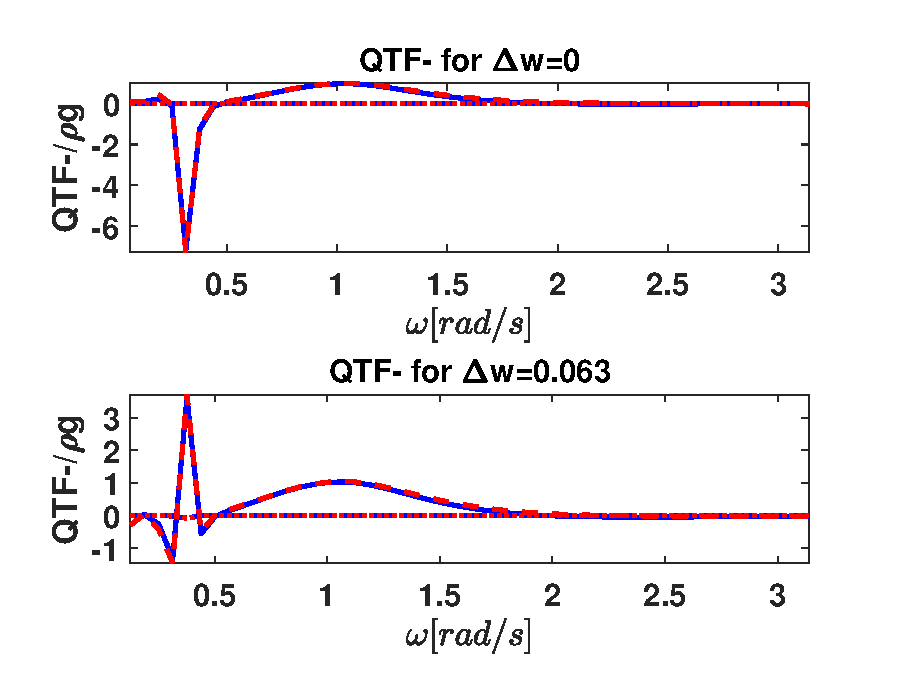
\includegraphics[scale=0.5,trim = 5mm 10mm 5mm 56mm, clip]{figures/Softwind/QTFM_Heave_beta030_diag.eps}	
}
\subfigure{
	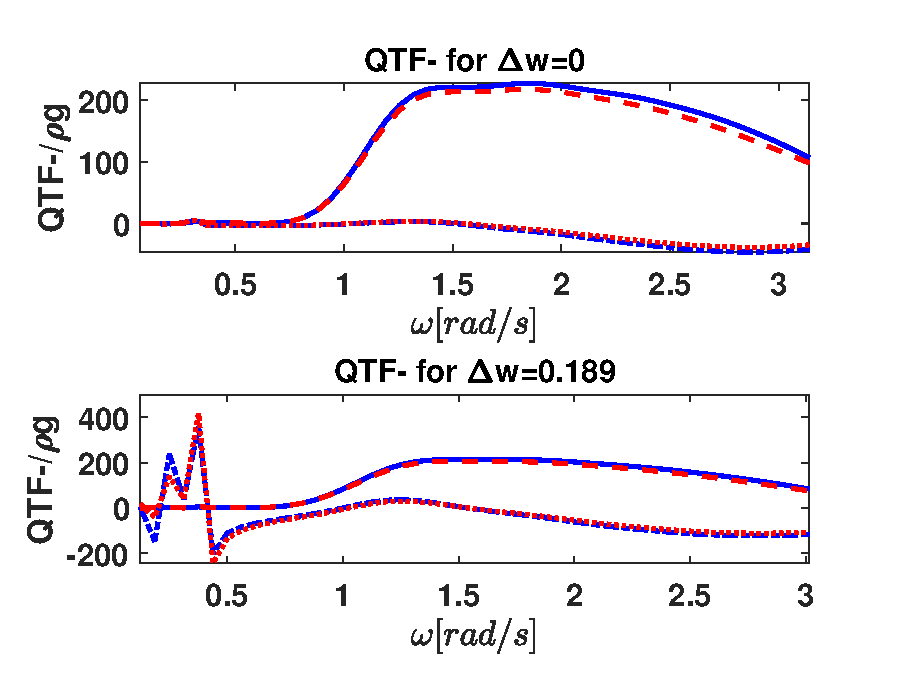
\includegraphics[scale=0.5,trim =1mm 2mm 5mm 56mm, clip]{figures/Softwind/QTFM_Pitch_beta030_diag.eps}	
}
	\caption{Comparison of the off-diagonal bi-directional, $(\beta_1,\beta_2)=(0^{\circ},30^{\circ})$, difference frequency QTF for the SOFTWIND platform (test case \textbf{10a\_QTF\_SOFTWIND}) between HYDROSTAR, real part (blue, solid-line), imaginary part (blue, dashed-dot line) and NEMOH, real part (red, dashed-line), imaginary part (red, dotted-line). On the top-left is for surge, on the top-right for heave (the first off-diagonal) and the bottom for pitch (the third off-diagonal)}\label{fig:QTFM_diag_softwind}
\end{figure}



\item \textbf{10b\_QTF\_SOFTWIND\_FS}: half symmetric body mesh without lid panels, half symmetric free-surface mesh, CoG $(0,0,-71.56)$, water depth 200 m, wave direction $0^{\circ}$, the sum-frequency total QTF DUOK+HASBO+HASFS+ASYMP. The results are shown in the density plot, Fig. \ref{fig:QTFP_SOFTWIND} and in the off-diagonal line plot, Fig. \ref{fig:QTFP_SOFTWIND_DIAG}. The mesh used was obtained using GMSH \cite{gmsh} and is shown in Fig. \ref{fig:meshesSoftwind}.



\begin{figure}[h!tbp]
	\centering
\subfigure{
	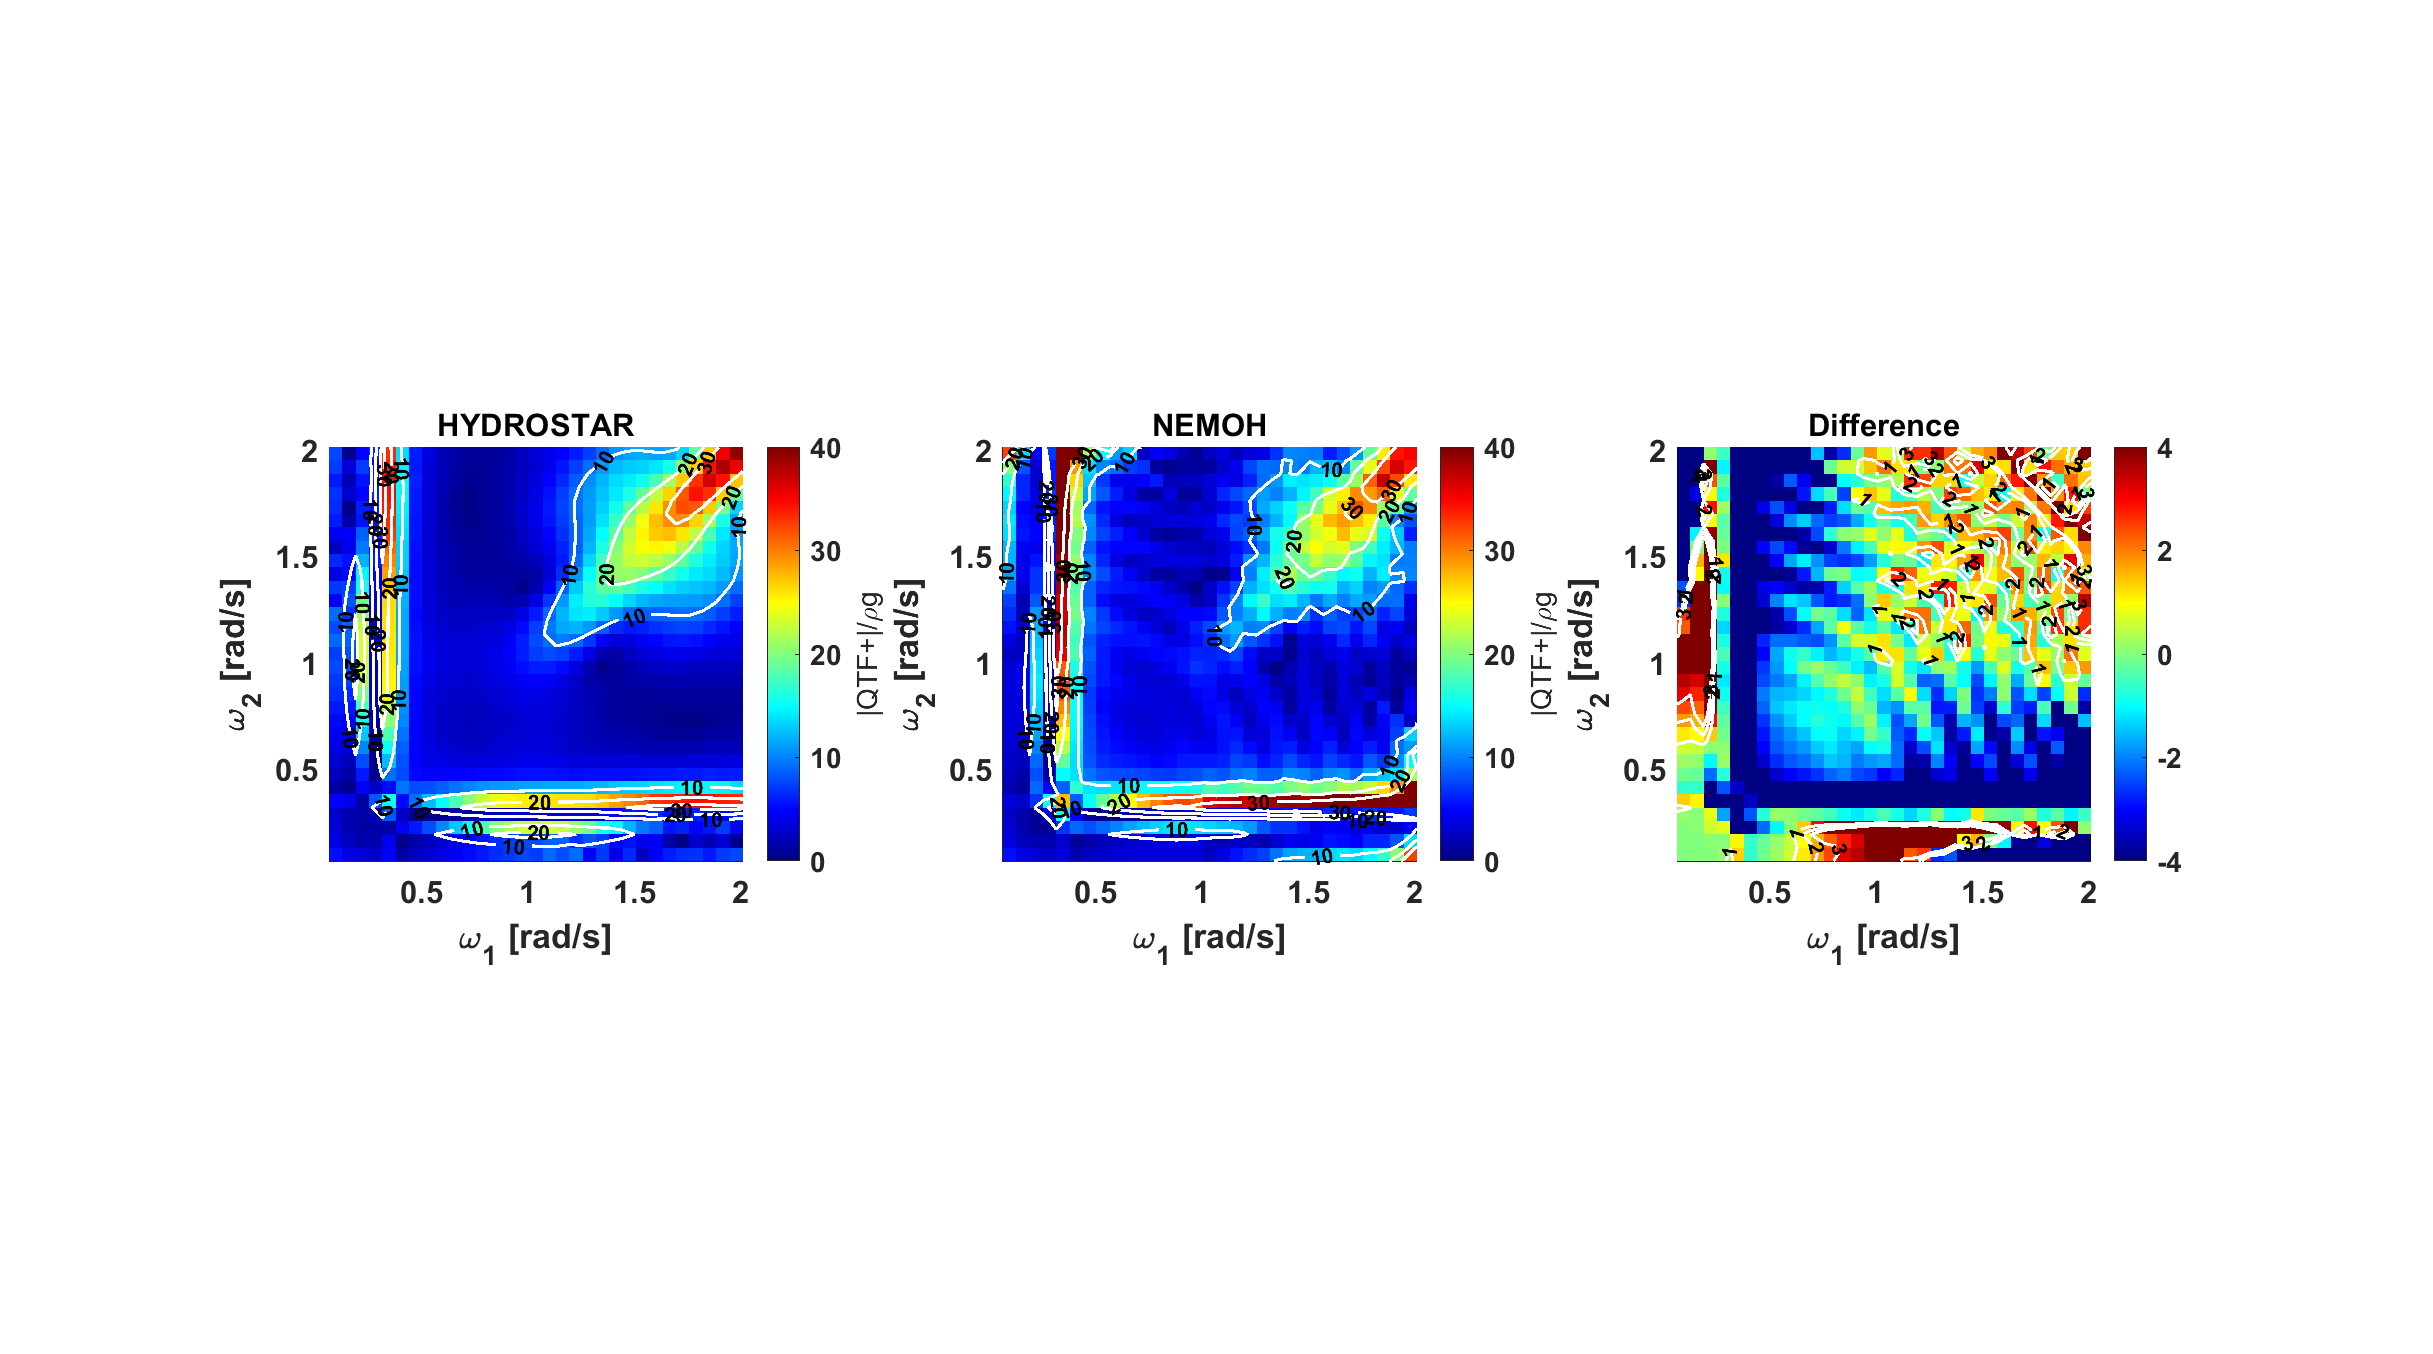
\includegraphics[scale=0.4,trim = 20mm 72mm 20mm 59mm, clip]{figures/Softwind/QTFP_Surge_beta00.eps}	
}
\subfigure{
	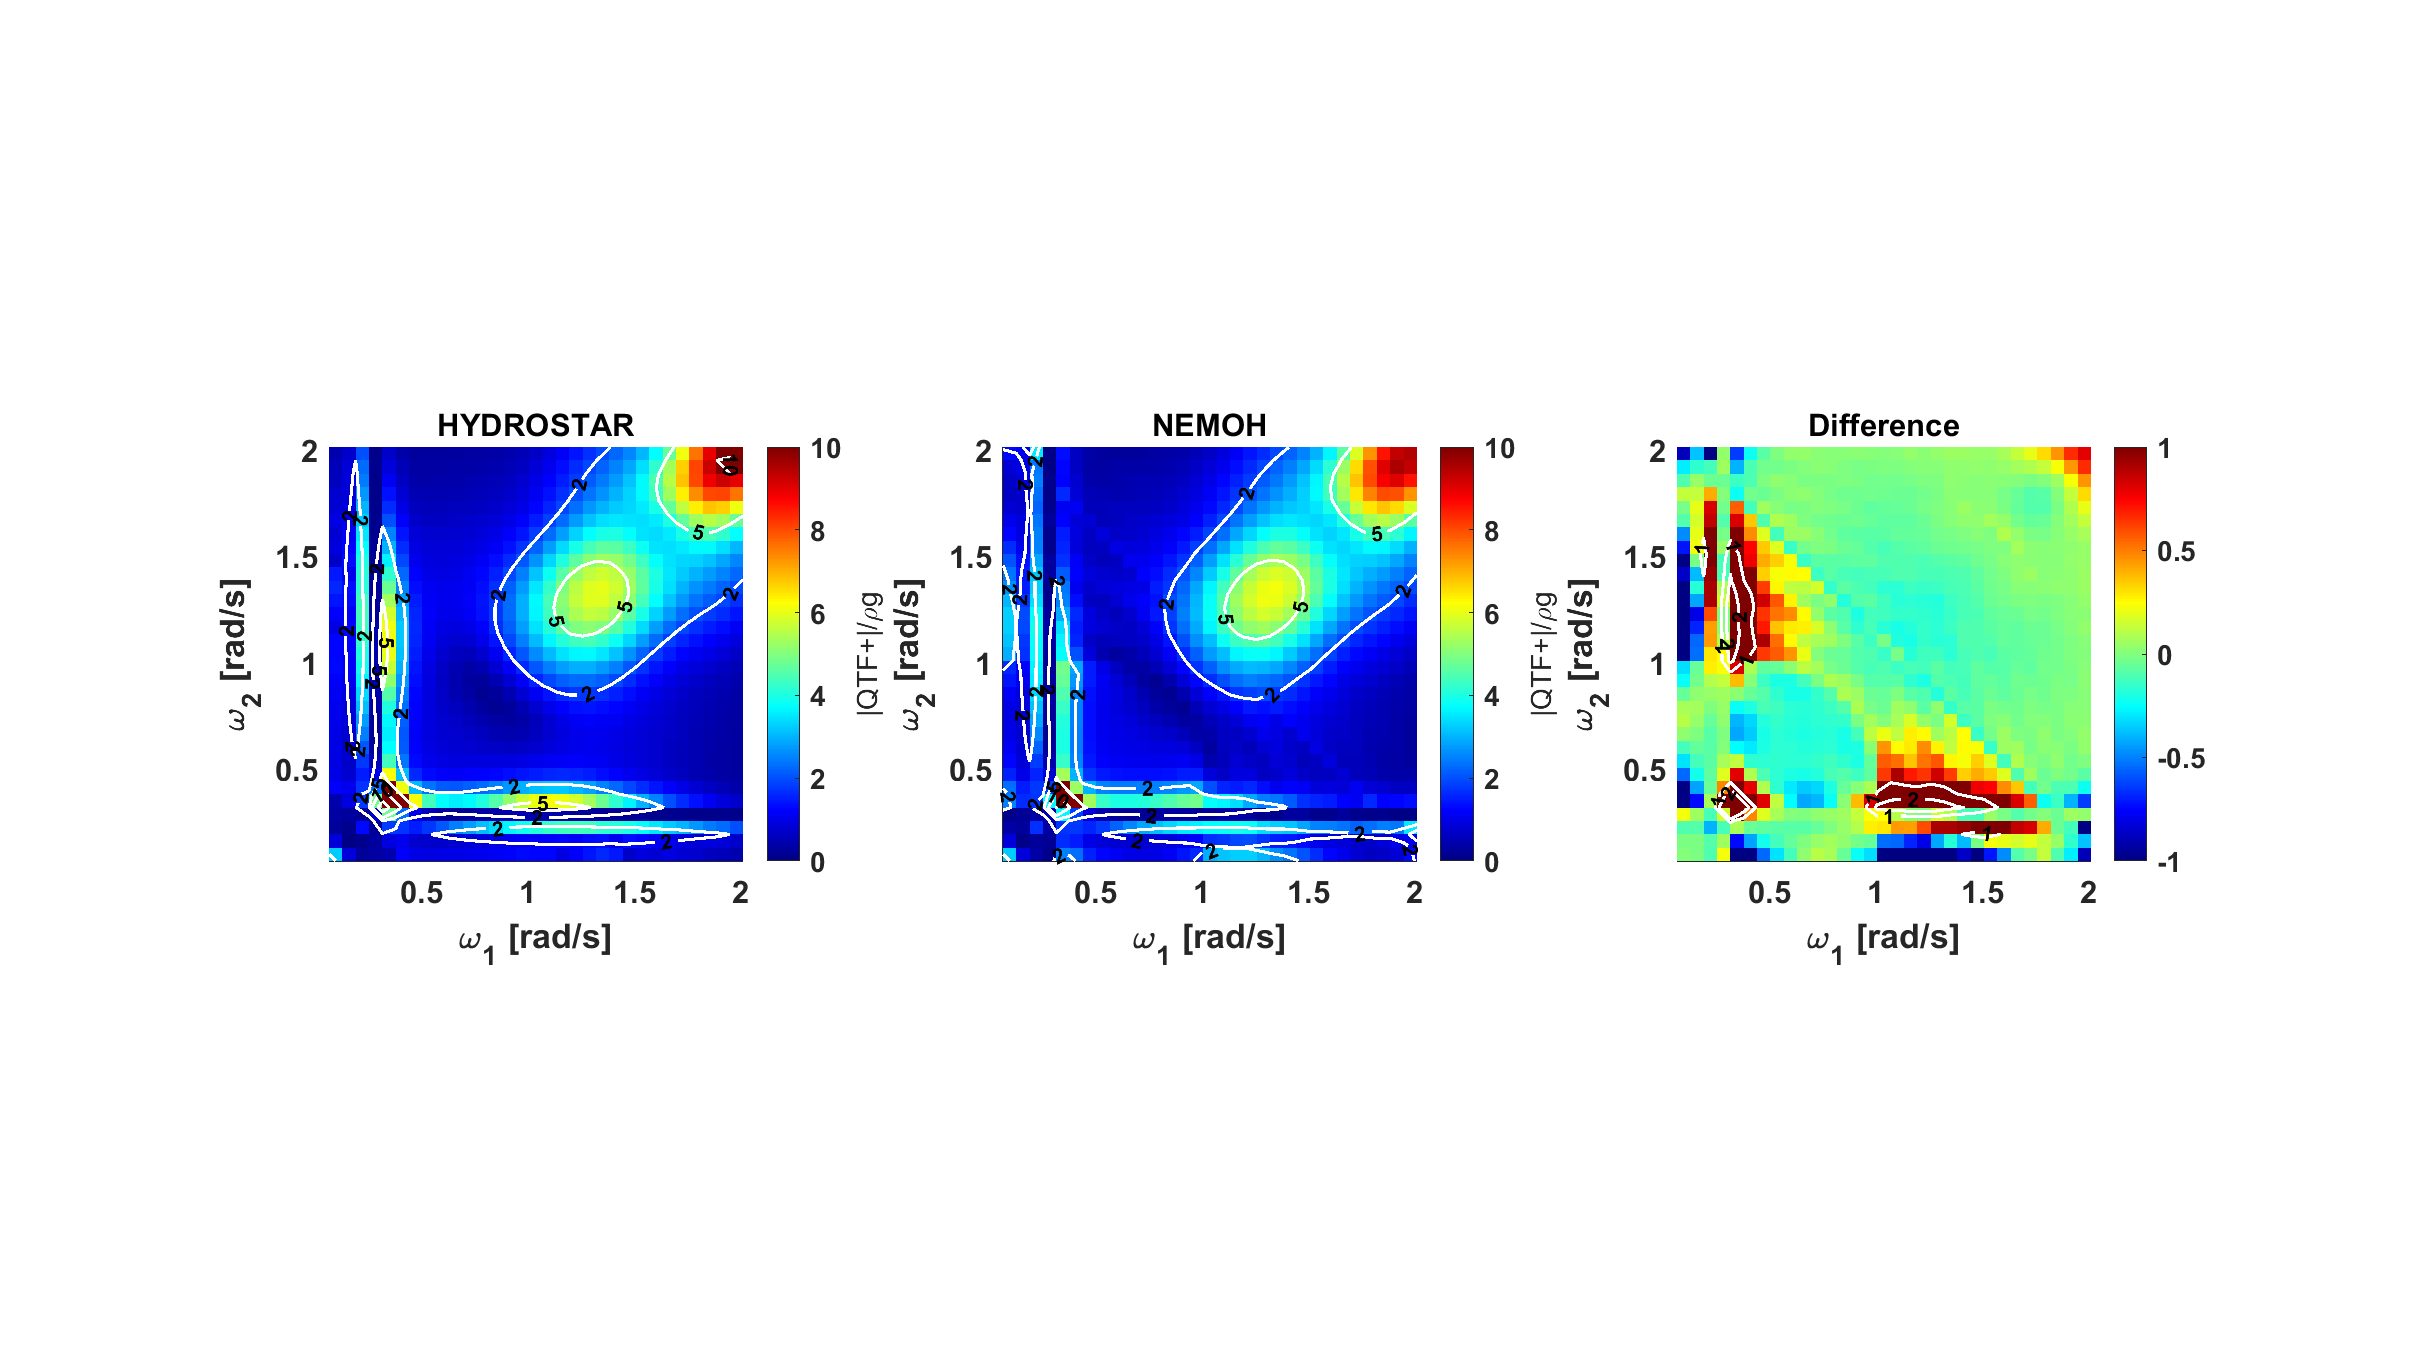
\includegraphics[scale=0.4,trim = 20mm 72mm 20mm 71mm, clip]{figures/Softwind/QTFP_Heave_beta00.eps}	
}
\subfigure{
	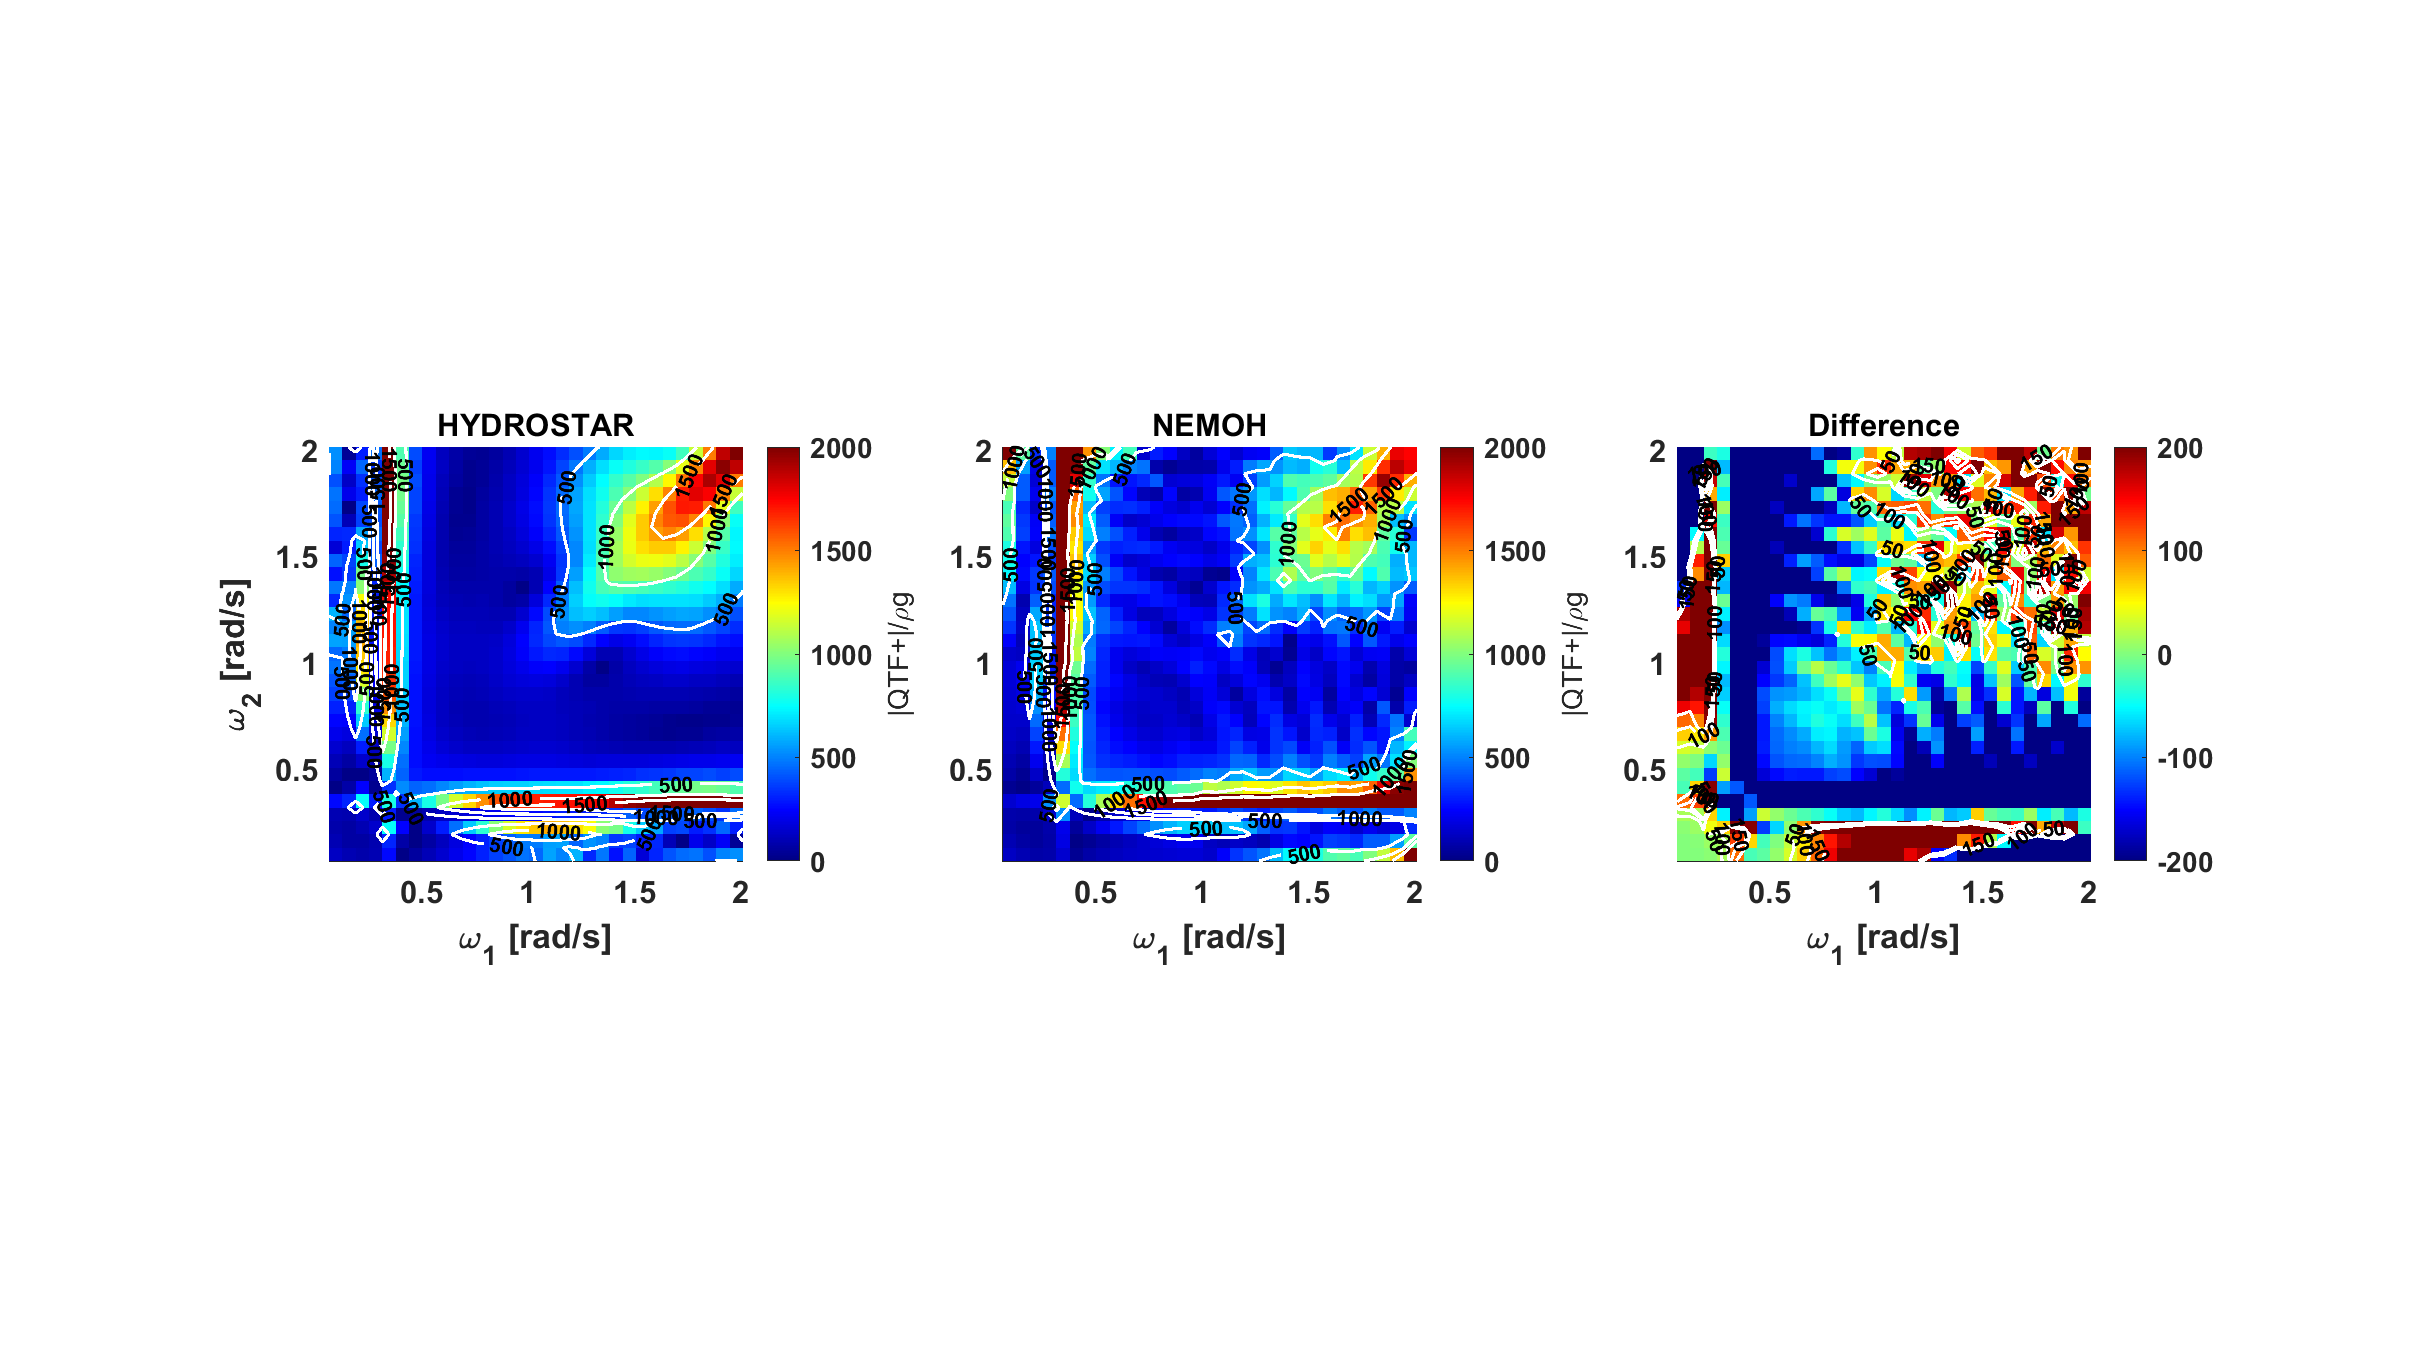
\includegraphics[scale=0.4,trim = 20mm 62mm 20mm 71mm, clip]{figures/Softwind/QTFP_Pitch_beta00.eps}	
}
	\caption{Density plots of the normalized sum-frequency full QTF magnitude (including the free-surface integrals) for the floating SOFTWIND platform (test case \textbf{10b\_QTF\_SOFTWIND\_FS}); on the top, middle and bottom row are for surge, heave and pitch, respectively. HYDROSTAR results are on the left column, NEMOH results are on the middle column and the difference in the right column.}\label{fig:QTFP_SOFTWIND}
\end{figure}

\begin{figure}[h!tbp]
	\centering
\subfigure{
	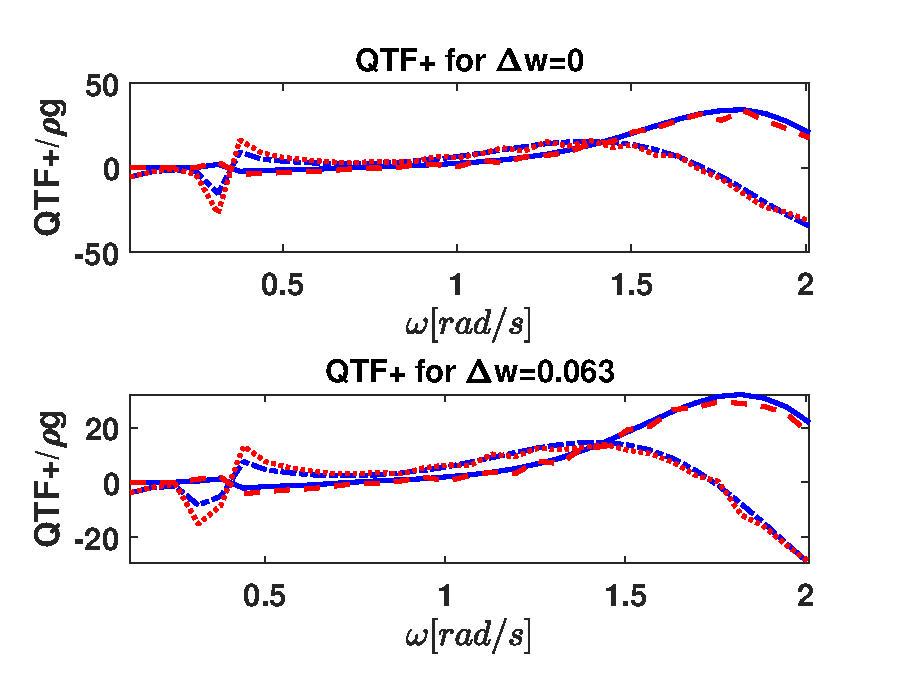
\includegraphics[scale=0.5,trim = 2mm 10mm 5mm 56mm, clip]{figures/Softwind/QTFP_Surge_beta00_diag.eps}	
}
\subfigure{
	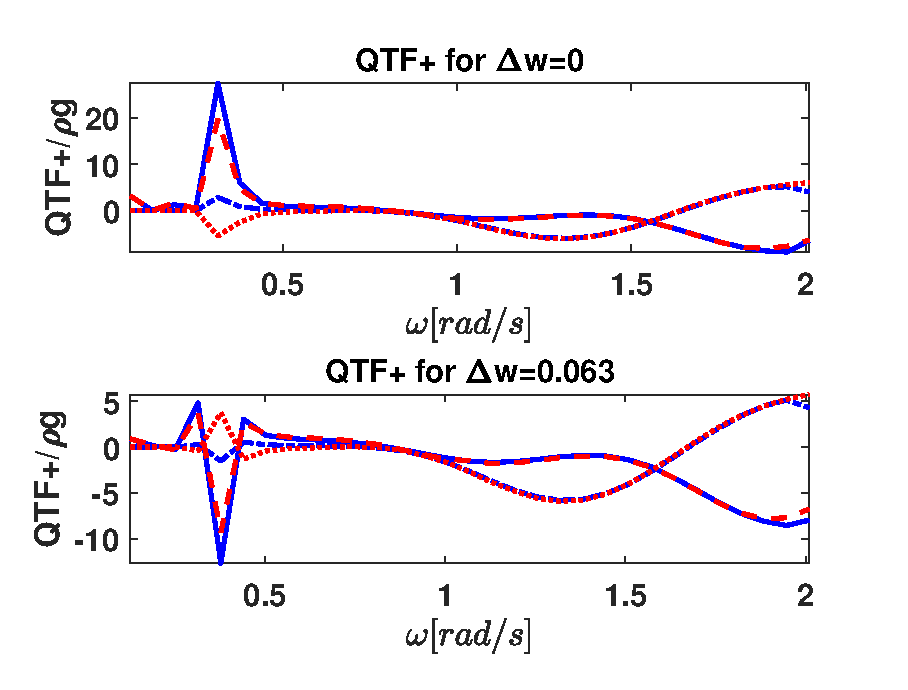
\includegraphics[scale=0.5,trim = 2mm 10mm 5mm 56mm, clip]{figures/Softwind/QTFP_Heave_beta00_diag.eps}	
}
\subfigure{
	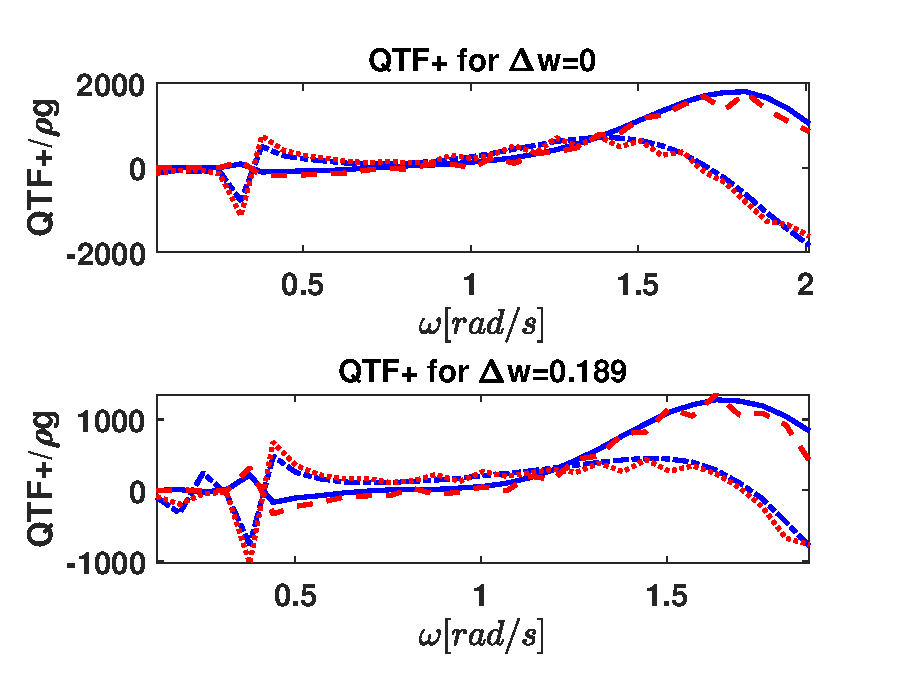
\includegraphics[scale=0.5,trim = 2mm 10mm 5mm 56mm, clip]{figures/Softwind/QTFP_Pitch_beta00_diag.eps}	
}
	\caption{Comparison of the off-diagonal sum-frequency full QTF for SOFTWIND platform (test case \textbf{10b\_QTF\_SOFTWIND\_FS}) between HYDROSTAR, real part (blue, solid-line), imaginary part (blue, dashed-dot line) and NEMOH, real part (red, dashed-line), imaginary part (red, dotted-line). On the top-left is for surge, on the top-right for heave (the first off-diagonal) and the bottom for pitch (the third off-diagonal)}\label{fig:QTFP_SOFTWIND_DIAG}
\end{figure}


\item \textbf{11\_QTF\_OC3\_Hywind}: full body mesh with lid panels, CoG $(0,0,0)$, water depth 320 m, wave direction $0^{\circ}$, NEMOH1 uses GMRES solver, the difference-frequency QTF DUOK+HASBO. The results are shown in the density plot, Fig. \ref{fig:QTFM_OC3_HYWIND} and in the off-diagonal line plot, Fig. \ref{fig:QTFM_diag_OC3_HYWIND}, of the difference-frequency QTF. The mesh used was obtained using GMSH \cite{gmsh} and is shown in Fig. \ref{fig:meshesHYWIND}.
\end{itemize}

\begin{figure}[h!tbp]
%\subfigure{
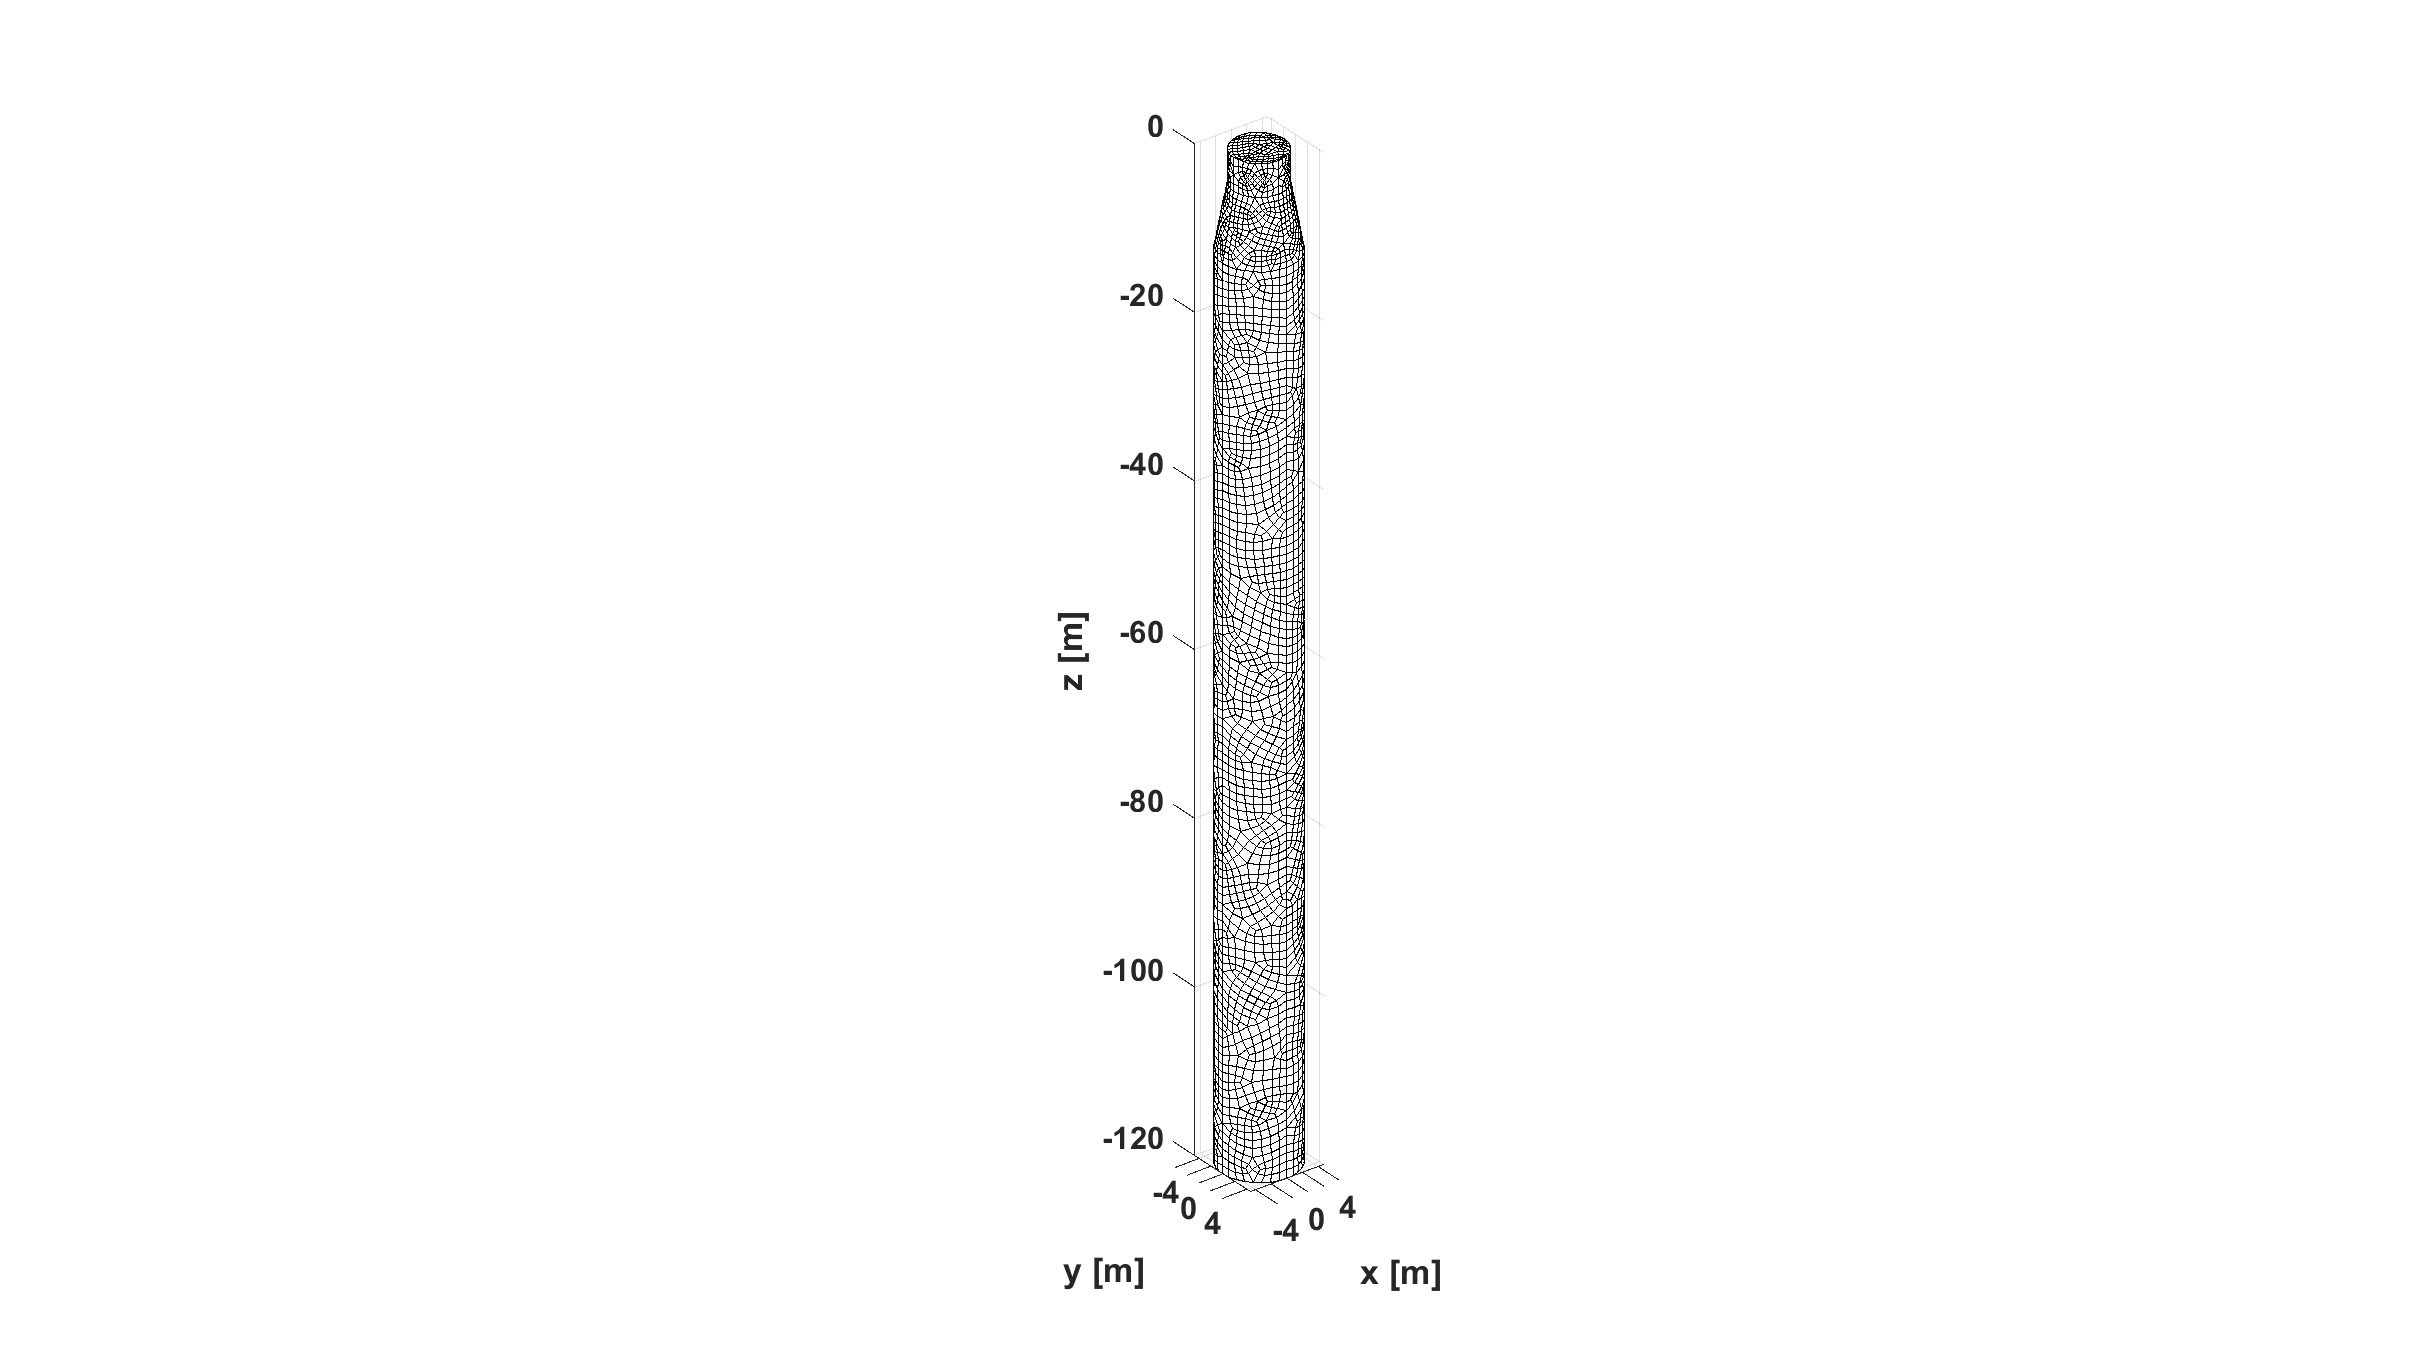
\includegraphics[scale=0.5,trim = 160mm 0mm 160mm 0mm, clip]{figures/OC3_HYWIND/bodyMesh.eps}	
%} 
\caption{Body boundary mesh for OC3-HYWIND platform, test case \textbf{11\_QTF\_OC3\_Hywind}.}\label{fig:meshesHYWIND}
\end{figure}

\begin{figure}[h!tbp]
	\centering
\subfigure{
	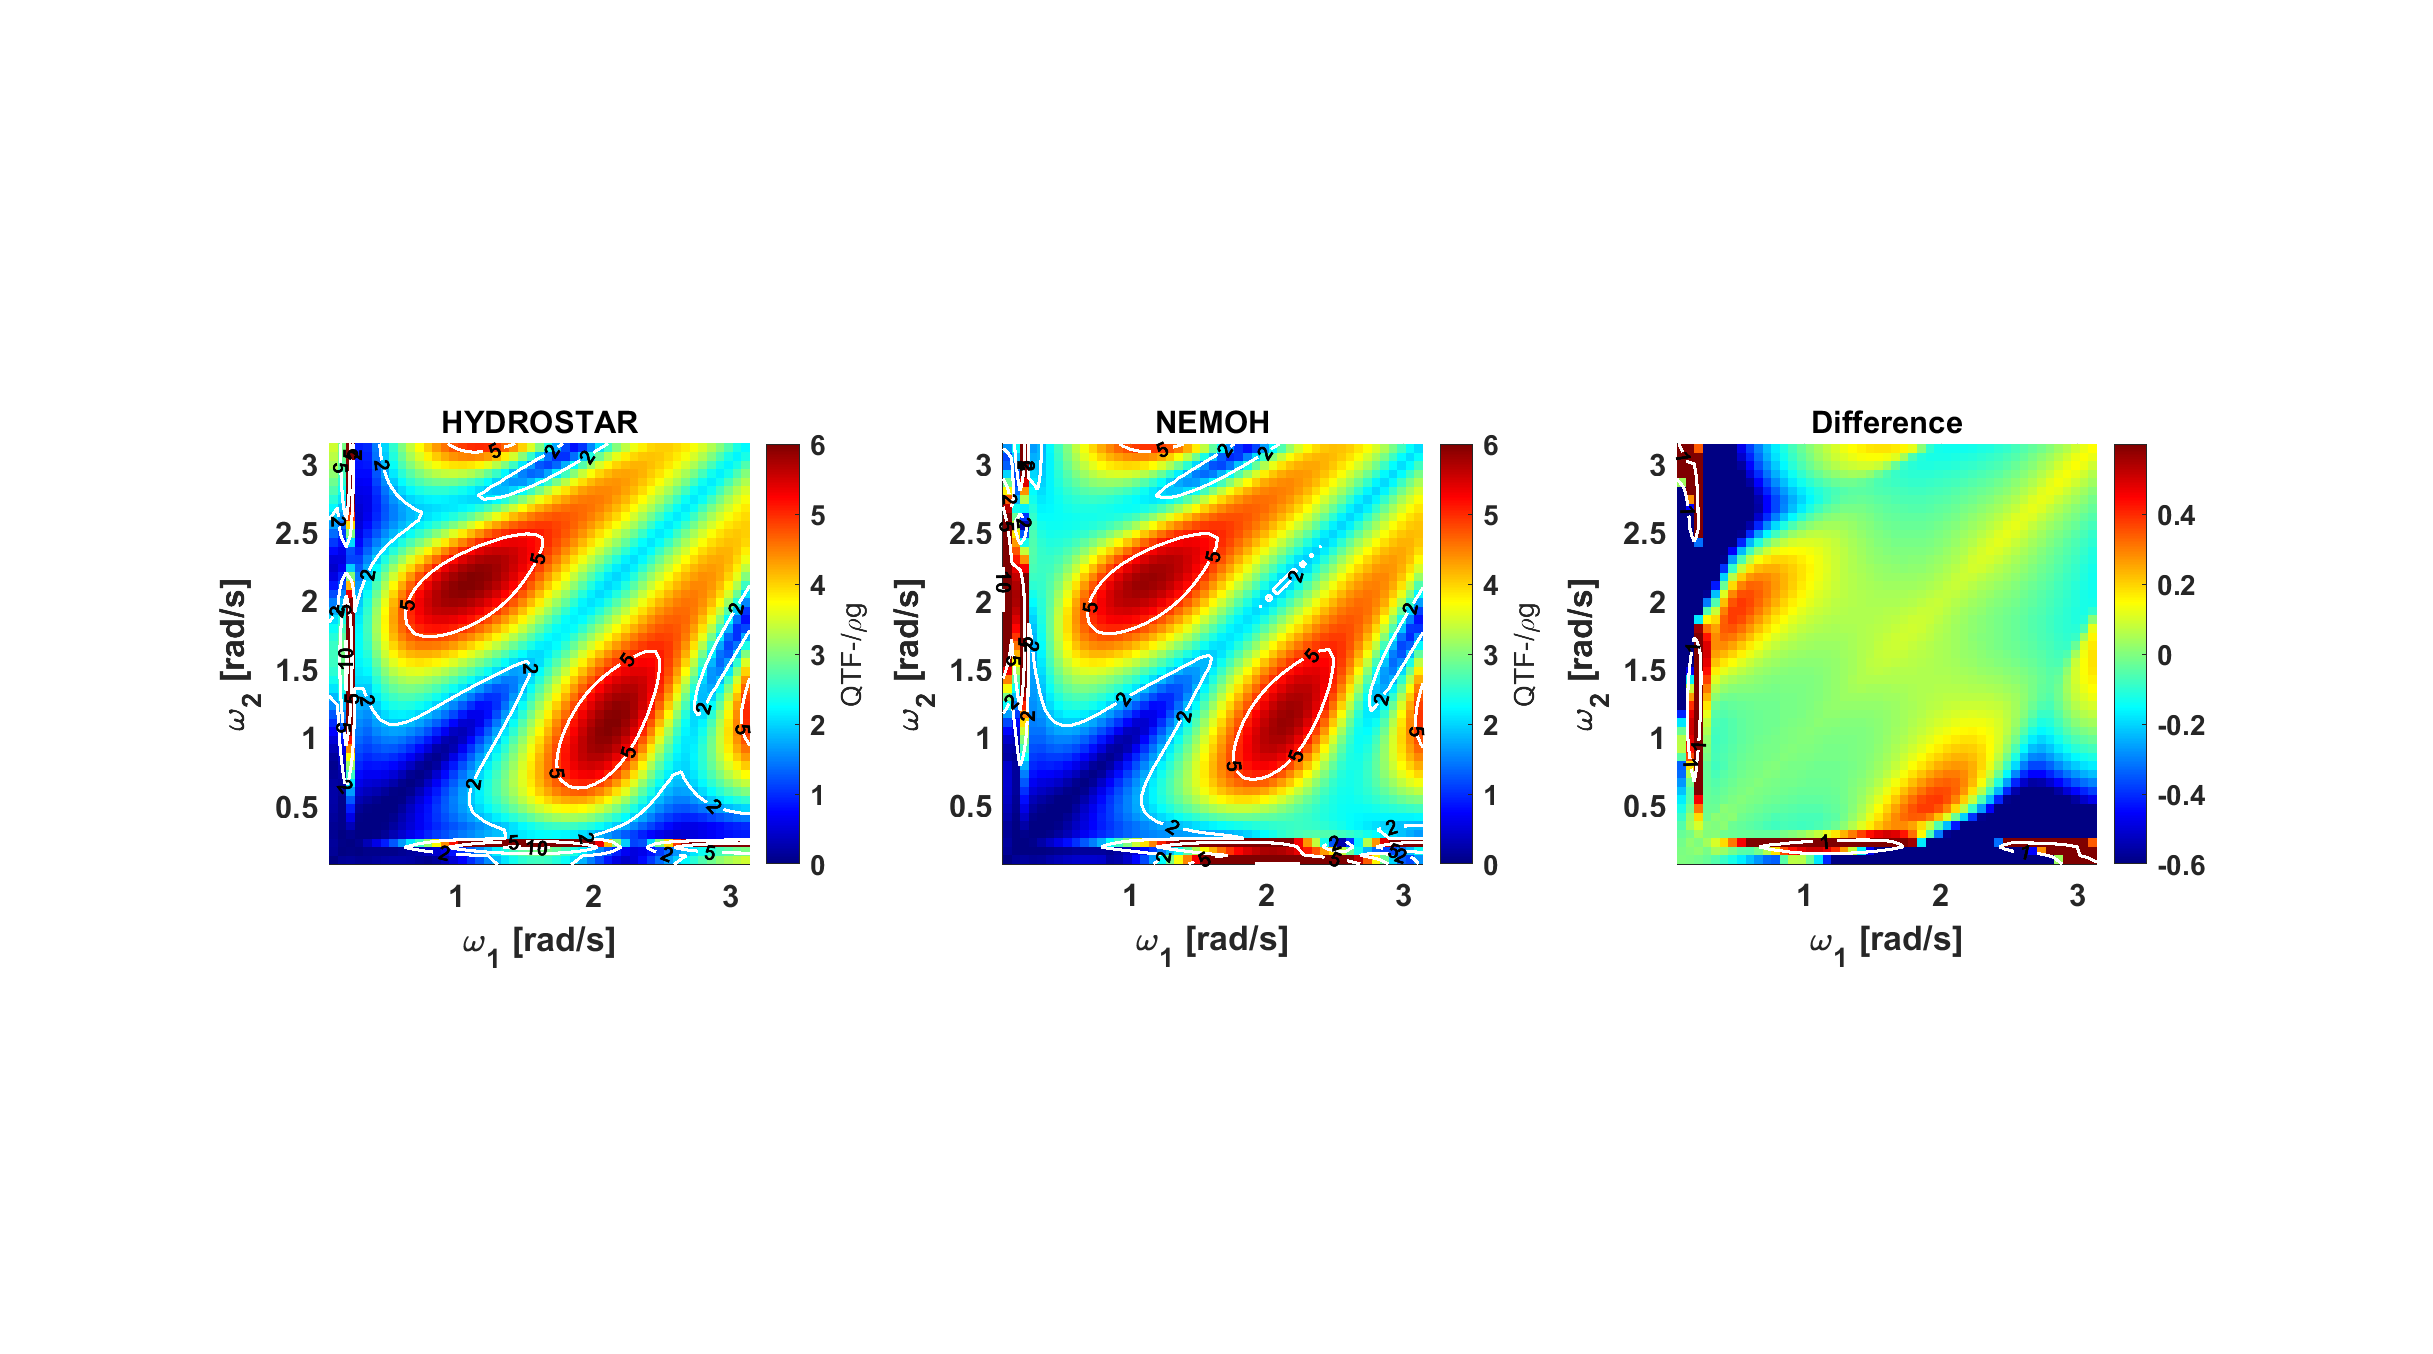
\includegraphics[scale=0.4,trim = 20mm 72mm 25mm 59mm, clip]{figures/OC3_HYWIND/QTFM_Surge.eps}
}
\subfigure{
	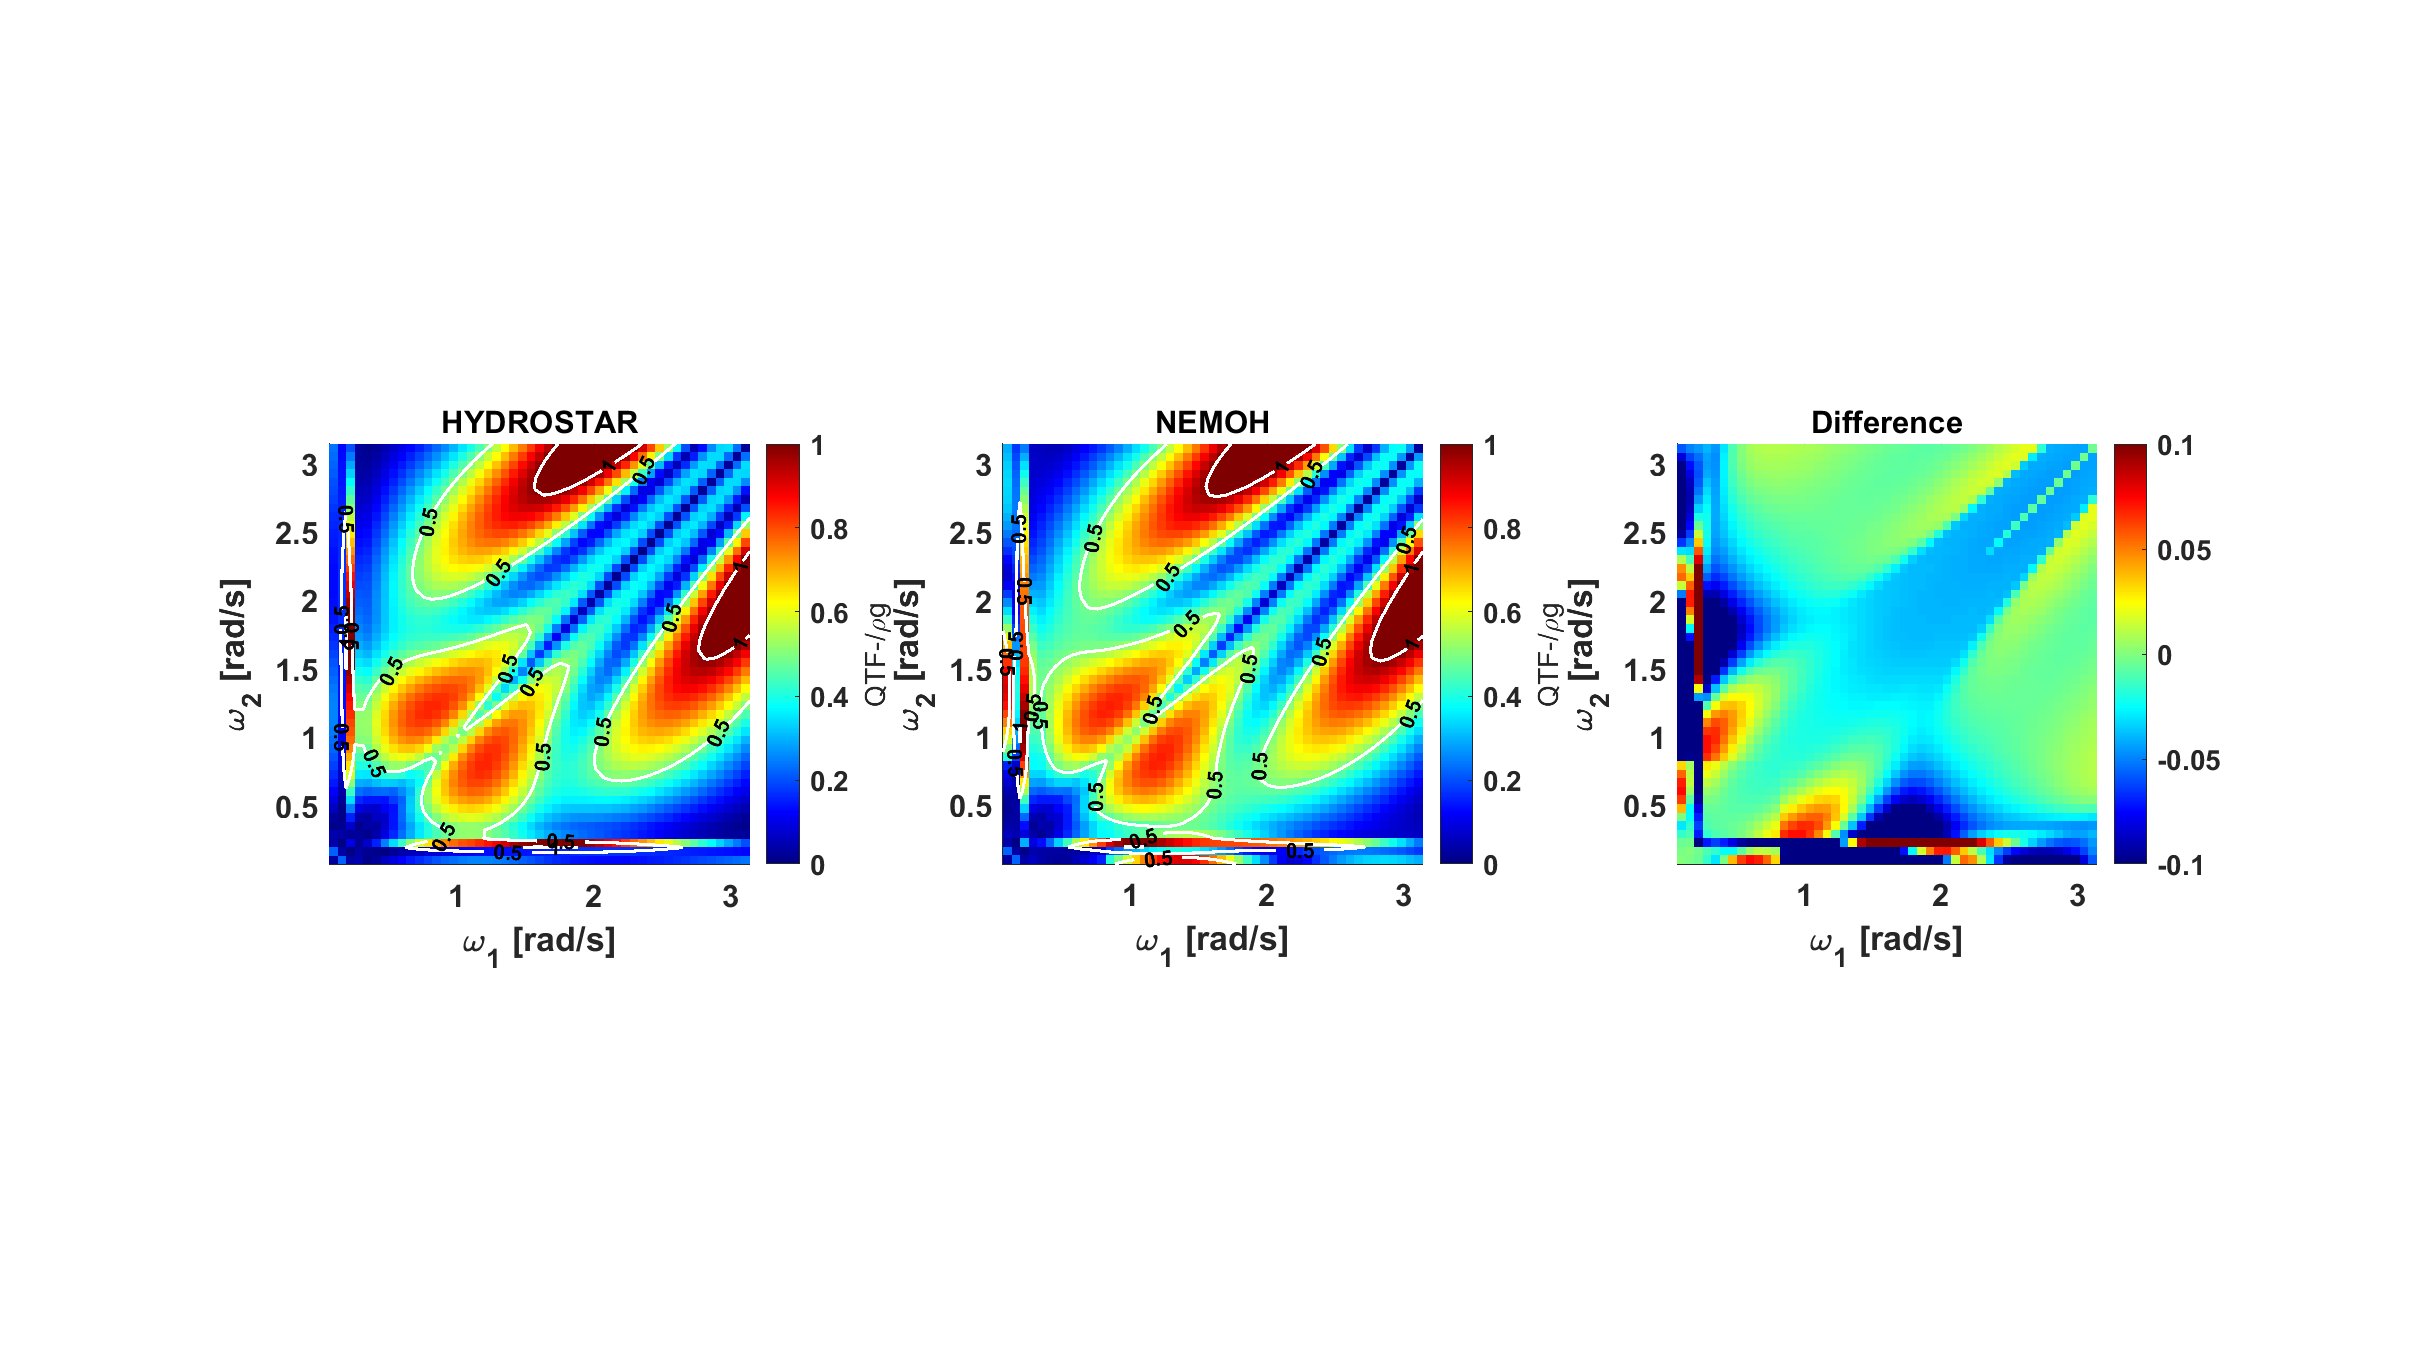
\includegraphics[scale=0.4,trim = 20mm 72mm 20mm 71mm, clip]{figures/OC3_HYWIND/QTFM_Heave.eps}	
}
\subfigure{
	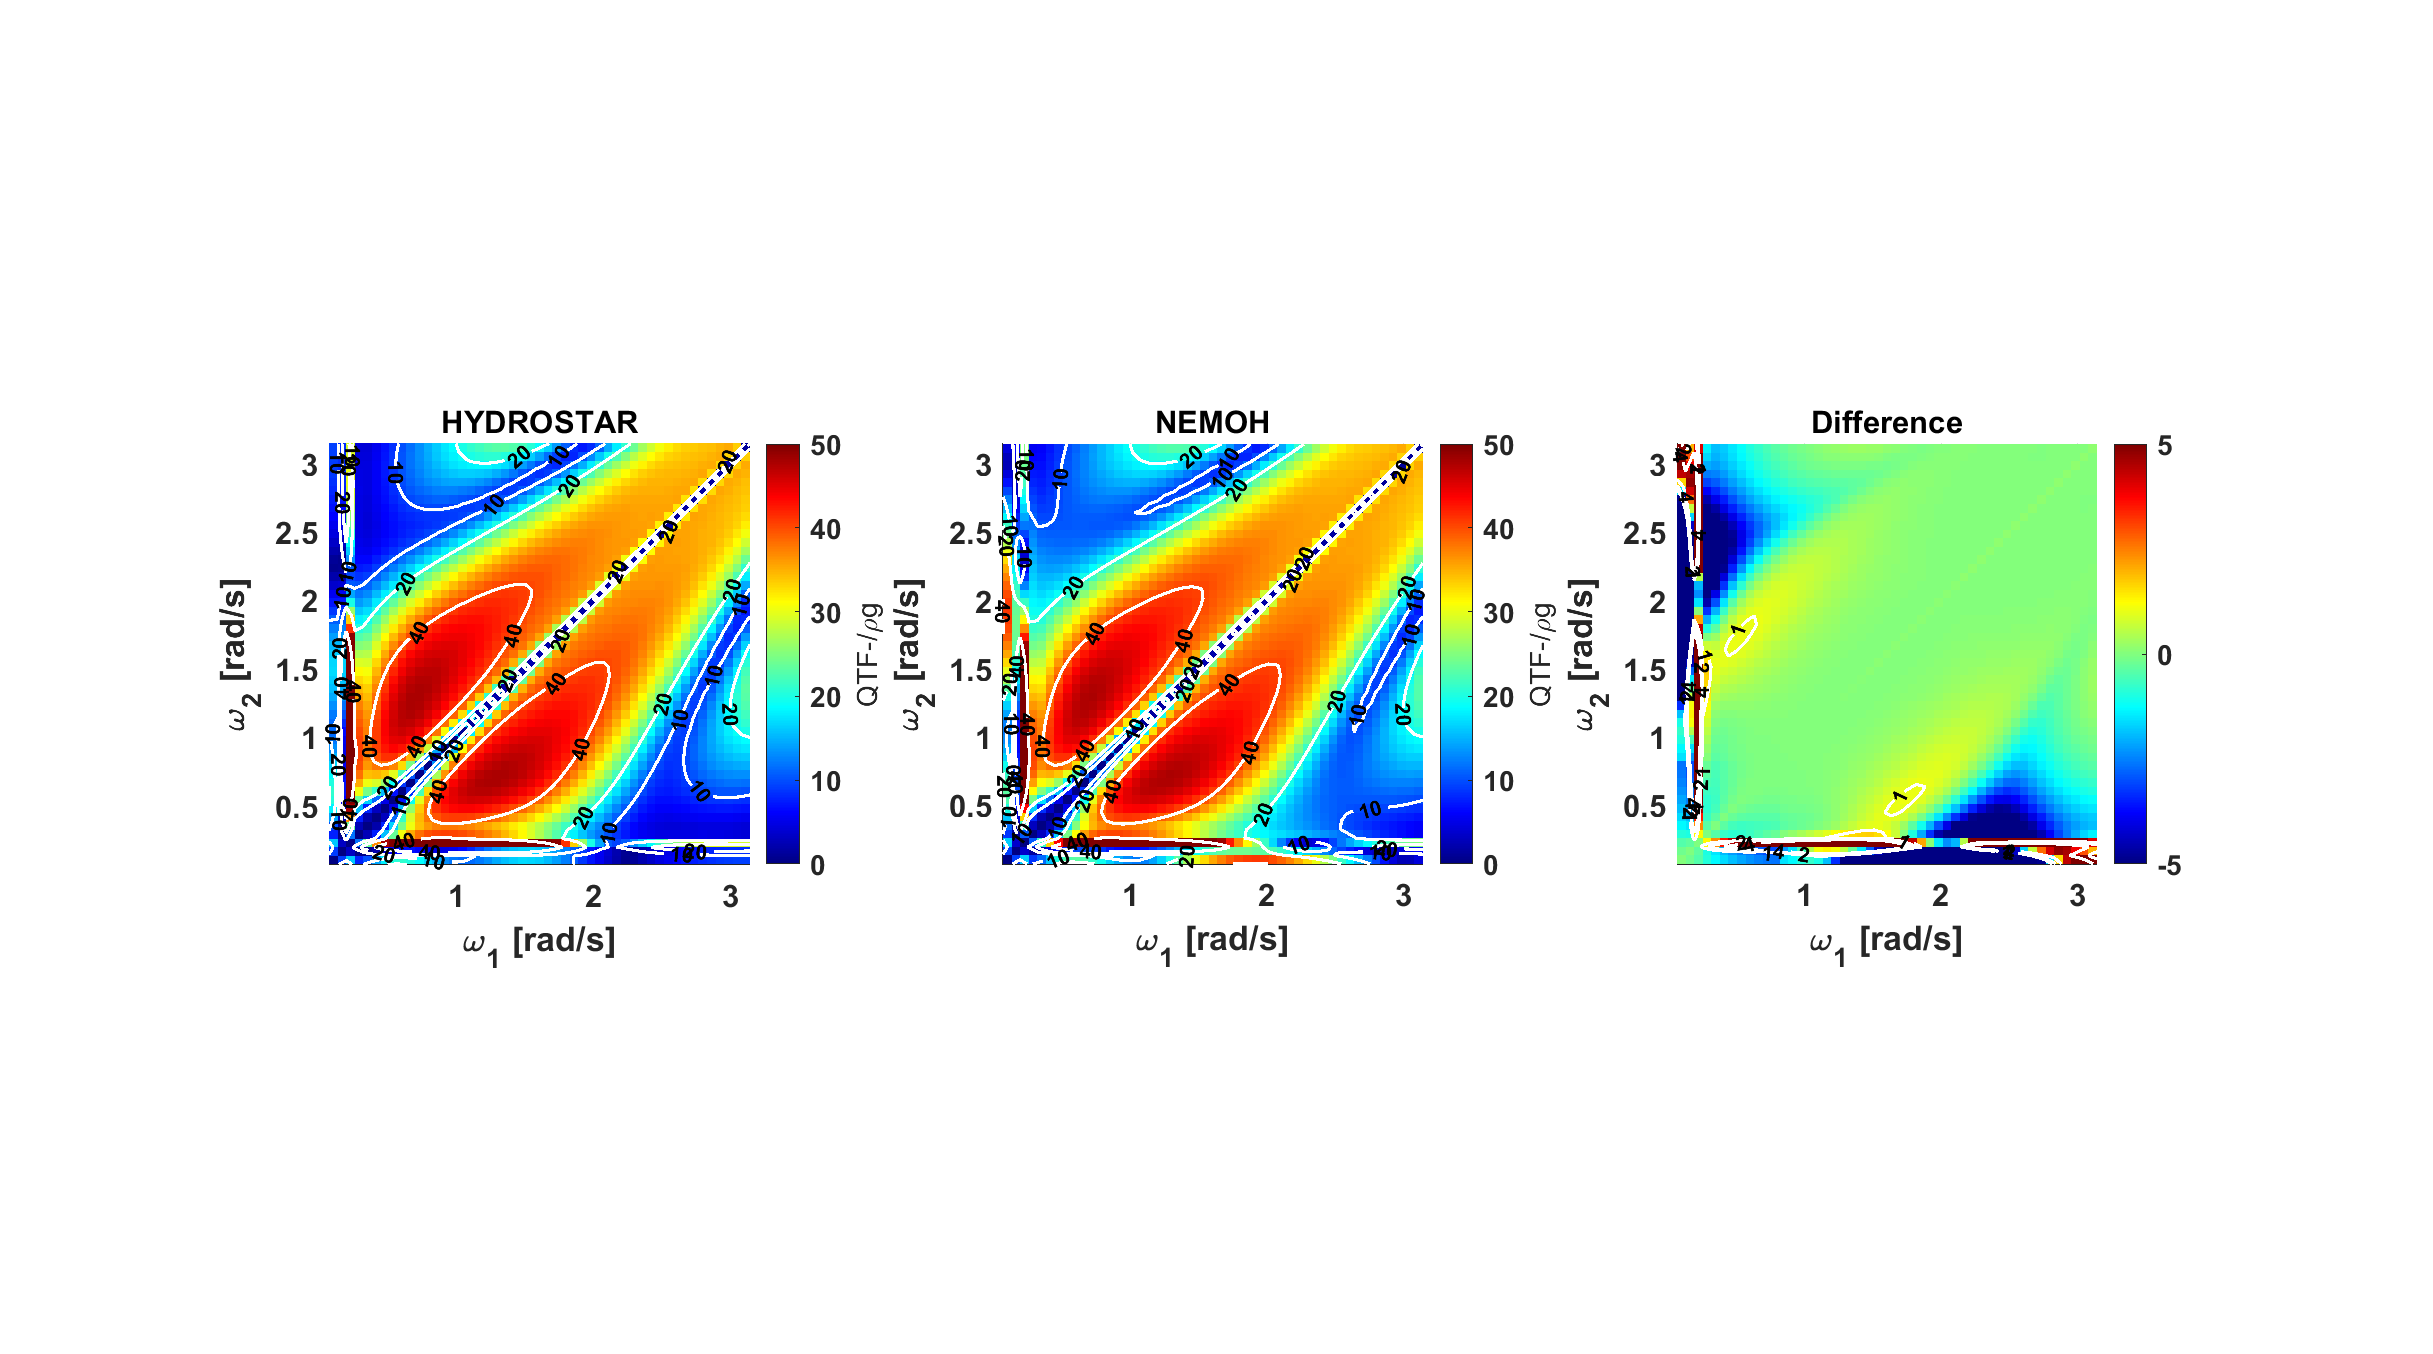
\includegraphics[scale=0.4,trim = 20mm 62mm 20mm 71mm, clip]{figures/OC3_HYWIND/QTFM_Pitch.eps}	
}
	\caption{Density plots of the normalized surge difference frequency QTF magnitude (without the free-surface integrals) for the floating OC3-HYWIND platform (test case \textbf{11\_QTF\_OC3\_Hywind}); on the top, middle and bottom rows are for surge, heave and pitch, respectively. HYDROSTAR results are on the left column, NEMOH results are on the middle column and the difference on the right column.}\label{fig:QTFM_OC3_HYWIND}
\end{figure}
\begin{figure}[ht!]
	\centering
\subfigure{
	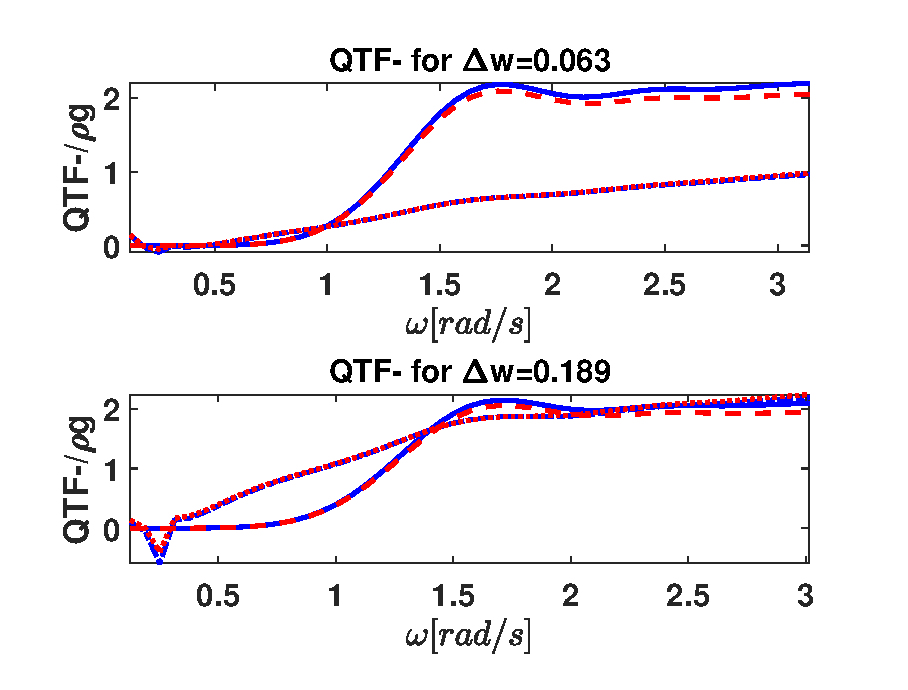
\includegraphics[scale=0.5,trim = 5mm 56mm 5mm 0mm, clip]{figures/OC3_HYWIND/QTFM_Surge_diag.eps}	
}
\subfigure{
	\includegraphics[scale=0.5,trim = 5mm 56mm 5mm 0mm, clip]{figures/OC3_HYWIND/QTFM_Heave_diag.eps}
}
\subfigure{
	\includegraphics[scale=0.5,trim =1mm 2mm 5mm 56mm, clip]{figures/OC3_HYWIND/QTFM_Pitch_diag.eps}
}
	\caption{Comparison of the off-diagonal difference frequency QTF for the OC3-HYWIND platform (test case \textbf{11\_QTF\_OC3\_Hywind}) between HYDROSTAR, real part (blue, solid-line), imaginary part (blue, dashed-dot line) and NEMOH, real part (red, dashed-line), imaginary part (red, dotted-line). On the top-left is for surge, on the top-right for heave (the first off-diagonal) and the bottom for pitch (the third off-diagonal)}\label{fig:QTFM_diag_OC3_HYWIND}
\end{figure}

Full description of the QTF test-cases results is reported in \citep{Kurnia22_JH,Kurnia22}. Note that the QTF comparisons between NEMOH and HYDROSTAR for the bidirectional case are in good agreement only if the direction is switched, in NEMOH $\beta=(\beta_1,\beta_2)$ and in Hydrostar $\beta=(\beta_2,\beta_1)$; further investigation regarding this is needed. The imaginary part of QTFs have also a difference sign between NEMOH and HYDROSTAR that may be due to different conventions of the incident potential. 

\FloatBarrier

\section*{Acknowledgement}
This work was done within the framework of the FLOATECH project. This project has received funding from the European Union’s Horizon 2020 research and innovation program under grant agreement No 101007142.

We thank Moran Charlou from LHEEA, ECN for his help in finalizing NEMOH v3.0 release in the gitlab.


\bibliographystyle{plain}
\bibliography{bibliography}


\end{document}